%--------------------------------------------------------------------------------------
%
%  Global settings, dont change it! (except additional \usepackage commands)
%  Always use PDFLatex!
%
%--------------------------------------------------------------------------------------
\documentclass[a4paper, 12pt, oneside, BCOR1cm,toc=chapterentrywithdots]{scrbook}

\usepackage{graphicx}
\usepackage{makeidx}
\makeindex
\usepackage[colorlinks=false]{hyperref}
\usepackage{tocbibind}
\usepackage{blindtext}
\usepackage{acronym}
\usepackage{amssymb}
\usepackage{tikz}
\usepackage{placeins}
\usepackage{subcaption}
\usetikzlibrary{positioning, arrows.meta}

\hypersetup{%
bookmarksnumbered=true, hyperindex=true,
bookmarksopen=true, bookmarksopenlevel=1,
pdfborder=0 0 0
}

\renewcommand*{\tableofcontents}{%
    \begingroup
    \tocsection
    \tocfile{\contentsname}{toc}
    \endgroup
}
\renewcommand*{\listoffigures}{%
    \begingroup
    \tocsection
    \tocfile{\listfigurename}{lof}
    \endgroup
}
\renewcommand{\listoftables}{
    \begingroup
    \tocsection
    \tocfile{\listtablename}{lot}
    \endgroup
}

\begin{document}

%--------titlepage
\begin{titlepage}
{
    \begin{center}
        \raisebox{-1ex}{
\includegraphics[scale=1.5]{TU_Chemnitz_positiv_gruen.pdf}}\\
    \end{center}
    \vspace{0.4cm}
}
\begin{center}
\LARGE{\textbf{AI-Augmented FAIRness Assessment of Research Software: A Hybrid Approach}}\\
\vspace{0.8cm}
\Large{\textbf{Master Thesis}}\\
\vspace{0.8cm}
Submitted in Fulfilment of the\\
Requirements for the Academic Degree\\
M.Sc.\\
\vspace{0.4cm}
Faculty of Computer Science\\
Chair of Distributed and Self-organizing Systems
\end{center}
\vspace{1.5cm}
Submitted by: Klea Haxhiu\\
Student ID: 858214\\
Submission Date: 28.09.2026\\
\vspace{0.5cm}\\
Examiner: Univ.-Prof. Dr. Martin Gaedke\\
Supervisor: Dr. Sheeba Samuel

\end{titlepage}

%---------------------------------------------------------
% Abstract
%---------------------------------------------------------
\addchap*{Abstract}
Automated assessment of FAIRness (Findability, Accessibility,
Interoperability, and Reusability) for research software has so far
relied primarily on rule-based tools that check for the presence of
structured metadata and repository artefacts. Such tools cannot assess
whether documentation --- most directly the README file --- clearly
communicates what a user needs to understand, install, use, and reuse
the software. This thesis addresses this limitation by proposing and
evaluating a hybrid FAIRness assessment framework for research software
repositories that combines deterministic structural checks with
large language model (LLM)-based assessment of qualitative
documentation characteristics.

The rule-based component evaluates six binary structural indicators
derived from the FAIR4RS principles: persistent identifiers,
structured metadata, licensing, dependency specifications, README
presence, and citation information. The LLM-based component evaluates
six documentation dimensions on a 0--2 ordinal scale: installation,
usage, purpose, dependencies, examples, and contribution guidance.
Rather than combining these components into a single scalar score,
the framework preserves them as a hybrid profile that reports
structural and documentation-based evidence separately.

The framework was applied to 188 research software repositories
collected from GitHub across ten research domains, with a manually
annotated corpus of 30 repositories used for evaluation. The
rule-based component achieved perfect agreement with the finalised
structural annotations. Two LLM configurations were evaluated against
the same qualitative rubric and README evidence: a locally hosted
Llama~3.1~8B model and
\texttt{Qwen3.6-35B-A3B-MLX-8bit}. Against the primary annotator,
their macro-average weighted Kappa values were 0.329 and 0.612,
respectively, compared with human--human agreement of 0.709. The
difference between the models, together with substantial variation
across documentation dimensions, shows that reliability is
model- and dimension-dependent. In particular, Qwen achieved strong
agreement for installation, purpose, and contribution information,
while examples and tutorials remained difficult under both
configurations and dependency documentation showed systematic
underscoring for Qwen. Self-reported confidence did not provide a
validated reliability signal for either configuration. No significant
repository-level relationship between README length and disagreement
was observed for either model.

The rule-based and documentation totals showed only weak and
statistically non-significant relationships for both Llama
($\rho=0.175$, $p=0.356$) and Qwen
($\rho=0.134$, $p=0.480$), consistent with the two components
contributing different information to the assessment, although these
results do not establish statistical independence.

In addition to the assessment pipeline, a web-based prototype was
implemented that presents dataset-level results, repository-level
hybrid profiles with supporting evidence, model comparison and
agreement statistics, and live assessment of public GitHub
repositories using either Llama or Qwen. Overall, the results show
that LLM-based assessment can extend automated FAIRness assessment
beyond structural repository checks, while its reliability must be
evaluated empirically for the model, documentation dimension, and
available evidence rather than assumed from aggregate performance or
self-reported confidence.
\par
\medskip
\noindent\textbf{Keywords:} FAIR, research software, large language models,
documentation quality, FAIRness assessment
%---------------------------------------------------------
% Table of Contents, List of figures, List of Tables
%---------------------------------------------------------
\tableofcontents
\listoffigures
\listoftables

%---------------------------------------------------------
% List of Abbreviations
%---------------------------------------------------------
\twocolumn
\addchap{List of Abbreviations}
\begin{acronym}[FAIR]
\acro{FAIR}{Findable, Accessible, Interoperable, Reusable}
\acro{FAIR4RS}{FAIR for Research Software}
\acro{LLM}{Large Language Model}
\acro{API}{Application Programming Interface}
\acro{README}{Read Me}
\acro{DOI}{Digital Object Identifier}
\end{acronym}
\onecolumn

%---------------------------------------------------------
% Here starts the real work
%---------------------------------------------------------

\chapter{Introduction}
\section{Motivation}

The increasing importance of open science and reproducibility has 
led to a growing need for effective management and reuse of digital 
research outputs, including data, software, and computational 
workflows. The FAIR principles — Findable, Accessible, Interoperable, 
and Reusable — were introduced by Wilkinson et al. \cite{wilkinson2016fair} 
to address these challenges by providing guidelines that enhance the 
discoverability and reuse of research artifacts. A central goal of 
the FAIR principles is machine-actionability — the ability of 
automated agents to discover, evaluate, and act on digital objects 
without prior knowledge of them.

While initially developed for research data, the FAIR principles are 
equally applicable to research software, which plays a central role 
in modern scientific processes. The FAIR for Research Software 
(FAIR4RS) principles \cite{barker2022fair4rs} extend and adapt the 
original framework to address the specific characteristics of 
software, such as executability, versioning, and dependency 
management. Ensuring that software is FAIR is essential for enabling 
reproducibility, transparency, and collaboration.

However, in practice, many research software repositories lack 
essential elements including structured metadata, clear licensing 
information, persistent identifiers, and comprehensive documentation. 
Assessing the FAIRness of research software at scale remains a 
challenging task, particularly for indicators that depend on the 
quality and completeness of software documentation 
\cite{chuehong2025frsm}.

Existing FAIRness assessment approaches primarily rely on rule-based 
checks that evaluate the presence of metadata files, licenses, 
persistent identifiers, and other objectively measurable indicators 
\cite{fuji2021}. While these approaches provide valuable automated 
assessments, they often struggle to evaluate qualitative aspects such 
as installation guidance, usage instructions, and documentation 
quality — factors that directly influence software reuse and 
reproducibility \cite{chuehong2025frsm}.

Recent advances in Large Language Models (LLMs) offer new 
opportunities for analyzing natural language documentation and 
supporting FAIRness assessment beyond traditional rule-based methods. 
By interpreting README files and other documentation artifacts, LLMs have the potential to evaluate aspects that are difficult to capture using deterministic rules alone.

This thesis investigates how LLM-based documentation assessment can
complement rule-based FAIRness evaluation for research software
through a hybrid assessment approach that combines automated
file-based checks with LLM-supported analysis of repository
documentation. The goal is to investigate whether LLM-based assessment
can capture qualitative FAIR-related documentation characteristics
that are not addressed by rule-based methods alone.

\section{Problem Statement}

Current automated methods for evaluating the FAIRness of research
software repositories are well suited to assessing explicit and
machine-detectable properties, but are more limited when information
is expressed in unstructured documentation. Existing automated
FAIRness assessment approaches commonly rely on deterministic checks
that evaluate the presence of metadata files, licenses, persistent
identifiers, and other objectively measurable indicators
\cite{fuji2021}. However, such approaches are not designed to assess
qualitative characteristics of software documentation, such as the
clarity and completeness of installation guidance, usage
instructions, or dependency information.

As noted by Chue Hong et al. \cite{chuehong2025frsm}, automated tools
can verify the existence of metadata, but presence alone does not
establish its quality, relevance, or usefulness.

Research on Mining Software Repositories has shown that README files 
are the primary documentation artifact for GitHub repositories and 
contain rich information about a project's purpose, usage, and 
quality \cite{prana2019readme}. However, the systematic integration of documentation-based information into automated FAIRness assessment workflows remains limited. 
Rule-based checks can readily verify whether a README file exists, but
presence-based checks alone do not determine whether it adequately
describes installation procedures, usage examples, or software
dependencies. Treude et al. 
\cite{treude2020beyond} further demonstrate that documentation 
quality goes beyond mere presence — dimensions such as clarity, 
understandability, and structure require qualitative assessment that 
rule-based approaches cannot provide.

The importance of documentation quality extends beyond academic 
frameworks. Imani et al. \cite{imani2024documentation} found that 
over 91\% of industry practitioners rely on OSS documentation for 
software adoption decisions, and that the top reported challenge is 
not the absence of documentation but the difficulty of finding 
relevant information within it. This practitioner evidence reinforces 
the need for assessment methods that evaluate not just the presence 
but the quality and completeness of documentation content.

Consequently, there is a need to investigate whether a hybrid approach
that combines rule-based structural checks with LLM-based qualitative
assessment can extend automated FAIRness evaluation to documentation
characteristics that are not captured by rule-based methods alone.

\section{Research Objective and Research Questions}
The primary objective of this thesis is to design, implement, and
evaluate a prototype system for the automated assessment of FAIRness
in research software repositories hosted on GitHub. The system
combines rule-based indicators derived from the FAIR4RS principles
\cite{barker2022fair4rs} with an LLM-based documentation assessment
component. The evaluation investigates both the extent to which
LLM-based assessment complements deterministic structural checks by
capturing qualitative documentation characteristics and the
reliability and failure modes of such assessment across two evaluated
LLM configurations.

The following research questions guide the investigation:

\begin{description}
    \item[RQ1] To what extent can LLM-based assessment complement
rule-based FAIRness assessment by capturing qualitative documentation
characteristics of research software repositories?
    
   \item[RQ2] How reliably can LLM-based methods assess qualitative
documentation dimensions of research software repositories, and what
failure modes affect their assessments?

\end{description}

The system is implemented as a modular Python prototype focused on 
GitHub-hosted repositories. Extensibility to other platforms such as 
Zenodo or Codeberg is considered out of scope for this thesis but is 
noted as a direction for future work.

\section{Thesis Structure}

The remainder of this thesis is organized as follows.

Chapter 2 reviews the relevant literature, covering the FAIR 
principles and their adaptation for research software, existing 
automated FAIRness assessment tools, research on software 
documentation quality, and recent advances in LLM-based document 
analysis.

Chapter 3 describes the proposed hybrid assessment approach, 
including the dataset collection methodology, the rule-based
component, the LLM-based documentation assessment component, and
the scoring and output design.

Chapter 4 describes the implementation of the proposed framework,
including the repository processing pipeline, rule-based assessment
component, LLM integration, generation of hybrid FAIRness profiles,
and the web-based prototype for exploring saved results and assessing
public GitHub repositories.

Chapter 5 presents the evaluation strategy and results, including
ground-truth validation, quantitative comparison of the evaluated
LLM configurations against manual annotations, analysis of
dimension-level scoring behaviour and failure patterns, and
comparison with existing FAIRness assessment tools.

Chapter 6 discusses the findings in relation to the research
questions, considers the implications and limitations of the
approach, and outlines directions for future work.

Chapter 7 concludes the thesis by summarising the main contributions
and findings.

\chapter{State of the Art}
This chapter reviews the literature relevant to the proposed hybrid
FAIRness assessment framework. It first introduces the FAIR principles
and their adaptation to research software, before examining existing
FAIRness assessment approaches, research on software documentation
quality, and LLM-based document analysis. Based on this literature,
the chapter derives the requirements for the proposed framework and
identifies the research gap addressed by this thesis.
\section{The FAIR Principles}

The FAIR principles were introduced by Wilkinson et al. 
\cite{wilkinson2016fair} as a minimal, domain-independent framework 
for improving the findability, accessibility, interoperability, and 
reusability of digital research objects. The principles were designed 
to support both human and machine interaction with research outputs, 
with machine-actionability as a central goal — the ability of 
automated agents to discover, evaluate, and act on digital objects 
without prior knowledge of them.

The four FAIR principles are defined as follows.

A digital object is \textbf{Findable} if it is assigned a globally 
unique and persistent identifier, described with rich metadata, and 
indexed in a searchable resource.

It is \textbf{Accessible} if it can be retrieved via an open and 
standardized protocol, and if its metadata remains accessible even 
when the object itself is no longer available.

\textbf{Interoperability} requires that the object uses formal 
knowledge representation languages, FAIR vocabularies, and qualified 
references to other objects.

Finally, an object is \textbf{Reusable} if it has rich attributes, 
a clear license, detailed provenance, and meets community standards.

An important characteristic of the FAIR principles is that they are 
modular and independent — they can be adopted incrementally and in 
any combination. Furthermore, FAIRness is treated as a continuum 
rather than a binary property: a digital object can be more or less 
FAIR depending on how completely it satisfies each principle. This 
continuum directly motivates the development of automated assessment 
tools capable of measuring FAIRness at scale.

The FAIR principles have become one of the most influential frameworks 
in research data management and open science. They have been adopted 
by funding agencies, research infrastructures, publishers, and 
scientific communities worldwide as a reference framework for 
improving the management and reuse of digital research outputs. Their 
widespread adoption has also motivated the development of FAIR 
assessment tools, metrics, and maturity indicators.

Despite their influence, the FAIR principles intentionally do not 
prescribe specific technologies, implementation strategies, or minimum 
compliance requirements. As a result, determining the degree of 
FAIRness of a digital object can be challenging and often requires 
interpretation. This has led to the development of automated 
assessment frameworks and community-specific implementations that 
translate the principles into measurable indicators.

While the FAIR principles were originally developed for research data, 
Wilkinson et al. explicitly noted their applicability to other 
scholarly digital objects including software, workflows, and 
algorithms. Consequently, while the FAIR principles provide a general 
conceptual framework, additional guidance is required to address 
software-specific characteristics and to enable meaningful FAIRness 
assessment of research software repositories.

\section{FAIR for Research Software}

Although the FAIR principles were originally formulated for research
data, their application to research software requires software-specific
interpretation. Research software is a living and complex research
object whose executability, versioning, dependencies, and continuing
evolution distinguish it from conventional research data
\cite{katz2021fair}. These characteristics make a direct application
of data-oriented FAIR practices insufficient and motivate dedicated
principles for research software.

To address these challenges, the FAIR for Research Software (FAIR4RS) 
principles were introduced by Barker et al. \cite{barker2022fair4rs}, 
building on earlier community discussion of how the FAIR principles 
apply to software \cite{lamprecht2020fairsoftware}.
The FAIR4RS principles were developed through a large community 
consultation process involving approximately 500 contributors from 
more than 110 organisations, reflecting broad international consensus 
on the need for software-specific FAIR guidance. The principles adapt 
the original framework to account for the unique characteristics of 
software, introducing new sub-principles where necessary.

Under FAIR4RS, software is \textbf{Findable} if it is assigned 
globally unique and persistent identifiers, with distinct identifiers 
for different versions and components — an extension not present in 
the original FAIR principles. Software is \textbf{Accessible} if it 
can be retrieved via standardised protocols and its metadata remains 
available even if the software itself becomes unavailable. 
\textbf{Interoperability} in FAIR4RS extends beyond metadata to 
include API interactions and references to related software objects. 
Finally, software is \textbf{Reusable} if it is executable, 
understandable, modifiable, and integrable into other systems, with 
clear licensing, provenance, and community standards.
Software identification and citation are also closely connected to
FAIRness. The Software Citation Principles emphasise software as a
legitimate research product and call for citations that support
credit, attribution, unique identification, persistence, and
accessibility \cite{smith2016softwarecitation}. These principles
reinforce the importance of persistent identifiers and citation
metadata in the FAIR assessment of research software.

Research software plays a critical role in enabling reproducible 
science, and FAIR4RS therefore positions software discoverability, 
accessibility, and reusability as essential requirements for 
transparent and reproducible research workflows.

A key insight of FAIR4RS is that FAIRness for software should begin 
during development rather than only at publication time. Unlike data, 
software may be used directly from its development environment, making 
early adoption of FAIR practices essential for reproducibility and 
reuse. The principles have received growing institutional support from 
organisations such as ELIXIR, ARDC, the Netherlands eScience Center, 
and ZB MED.

Despite this progress, FAIR4RS defines high-level principles without 
prescribing concrete automated assessment methods. Many FAIR4RS 
indicators rely on metadata and structural information, while 
qualitative aspects such as documentation clarity, installation 
guidance, and usage examples remain difficult to evaluate 
automatically. This gap between the principles and their practical 
assessment motivates the development of automated tools capable of 
evaluating both structured and unstructured aspects of research 
software repositories.

\section{Existing FAIRness Assessment Approaches}

Several tools and frameworks have been developed to automate the 
assessment of FAIRness for digital research objects. This section 
reviews the most relevant approaches, highlighting their capabilities 
and limitations in the context of research software assessment.

\subsection{FAIR Assessment Frameworks and Maturity Indicators}

The translation of the FAIR principles into measurable criteria has
been addressed by several general FAIR assessment frameworks.
Wilkinson et al. \cite{wilkinson2019evaluating} proposed a scalable
and automated evaluation framework based on community-defined FAIR
Maturity Indicators and associated compliance tests. The approach
demonstrates how high-level FAIR principles can be operationalised
through explicit, machine-actionable tests while retaining
metric-level assessment results.

The need for consistent operational criteria was further addressed by
the FAIR Data Maturity Model developed by Bahim et al.
\cite{bahim2020fairdmm}. The model provides a common set of indicators
and priorities intended to harmonise FAIR assessment approaches and
improve comparability between evaluations. Together, these works
illustrate an important transition from conceptual FAIR principles
towards explicit and reproducible assessment criteria. However, their
primary focus is FAIR assessment of data and digital research objects
rather than qualitative documentation assessment of research software
repositories.

\subsection{F-UJI}

F-UJI is an automated web-based FAIR assessment tool developed within 
the FAIRsFAIR initiative \cite{fuji2021}. It evaluates the FAIRness 
of digital research objects by performing machine-actionable checks 
against predefined metrics, producing quantitative scores across the 
four FAIR dimensions. F-UJI accepts persistent identifiers and 
metadata endpoints as input and evaluates indicators such as metadata 
presence, persistent identifiers, licensing, semantic vocabularies, 
provenance information, and accessibility protocols.

F-UJI treats FAIRness as a spectrum rather than a binary property, 
providing detailed metric-level reporting and evidence traces. It 
demonstrates that many aspects of FAIR compliance can be assessed 
automatically through metadata checks. However, F-UJI is primarily 
metadata-centric and was originally designed for FAIR digital objects 
and datasets rather than research software repositories specifically. 
It was not designed for direct GitHub repository assessment and 
expects persistent identifiers and structured metadata records as 
input, which many repositories in practice do not provide.

Critically, F-UJI evaluates the existence and machine-readability of 
metadata rather than its semantic quality or usefulness. Documentation 
quality, understandability, and usability are not assessed, creating 
a gap between structural FAIR compliance and meaningful software 
reusability.

\subsection{FAIR-IMPACT Metrics}

The FAIR-IMPACT initiative extended existing FAIR assessment 
approaches by defining 17 concrete, measurable FAIR Research Software 
Metrics (FRSM-01 to FRSM-17) for automated assessment of research 
software against the FAIR4RS principles \cite{chuehong2025frsm}. 
These metrics operationalize FAIR4RS into practical automated checks, 
covering findability, accessibility, interoperability, and 
reusability indicators at the code, project, and repository level.

The metrics use three compliance levels — Essential, Important, and 
Useful — and are designed to be domain-agnostic while adaptable to 
disciplinary contexts. Planned integration into F-UJI demonstrates 
their practical application potential. However, the FAIR-IMPACT 
metrics explicitly acknowledge that automated tools can verify the 
existence of metadata but cannot reliably determine its quality, 
relevance, or correctness. Qualitative aspects such as documentation 
clarity and usability remain outside the scope of automated rule-based 
assessment.

\subsection{FAIR-Aware}

In contrast to automated assessment tools, FAIR-Aware is a 
human-centred self-assessment tool \cite{akerman2021fairaware} developed within the FAIRsFAIR 
initiative that focuses on increasing FAIR literacy among researchers. 
It uses a questionnaire-based approach to help researchers reflect on 
how FAIR practices can be integrated into their workflows, providing 
guidance and recommendations rather than automated compliance metrics.

FAIR-Aware demonstrates that FAIRness assessment is not limited to 
verifying machine-readable metadata. Many FAIR considerations require 
researchers to interpret community standards, evaluate reuse 
conditions, and make contextual decisions that depend on domain 
knowledge and qualitative judgment. This highlights the importance of 
qualitative reasoning in FAIR evaluation — a dimension that automated 
rule-based tools cannot fully address.

\subsection{FAIRsharing}

FAIRsharing \cite{sansone2019fairsharing} is a curated registry of FAIR-related standards, 
repositories, databases, policies, and metadata schemas. It provides 
centralised infrastructure to support the discovery, adoption, and 
interconnection of community standards and FAIR-enabling resources 
across research domains. FAIRsharing demonstrates that FAIRness is 
deeply connected to the existence and adoption of shared standards 
and controlled vocabularies — automated FAIR assessment systems rely 
heavily on this ecosystem infrastructure to validate interoperability 
and machine-readability. FAIRsharing is particularly relevant for 
research software because it supports the discovery of community 
standards, metadata schemas, and domain-specific resources that 
contribute to software interoperability and reuse.

\subsection{howfairis}

howfairis \cite{spaaks2020howfairis} is a command-line tool developed
by the Netherlands eScience Center that evaluates a GitHub or GitLab
repository's compliance with the five fair-software.eu
recommendations: whether the repository is publicly accessible with
version control, whether a license file is present, whether the
software is registered in a community registry, whether citation information is available, for example through a
\texttt{CITATION.cff} file — a specification providing human- and
machine-readable citation metadata that developers can include
directly in a repository \cite{druskat2021cff} — and whether quality
checklist evidence is present.
Unlike F-UJI, howfairis operates directly on software repositories rather
than requiring a persistent identifier or metadata endpoint as input,
making it directly applicable to GitHub-hosted research software.

Like F-UJI and the FAIR-IMPACT metrics, howfairis restricts its
assessment to the presence of structural, machine-detectable evidence.
It does not evaluate the content or clarity of README documentation,
the completeness of installation or usage instructions, or any other
qualitative aspect of software reusability.

\subsection{Summary}

Existing FAIRness assessment tools provide valuable automated 
evaluation capabilities and have significantly advanced the practical 
application of FAIR principles. However, their primary focus remains 
on structured metadata and objectively measurable indicators, leaving 
qualitative aspects of software documentation largely unexplored.

\section{Software Documentation Quality}

While existing FAIRness assessment tools focus on structured metadata 
and file presence, research on software documentation quality 
highlights a complementary dimension of software reusability that 
these tools do not address. README files commonly act as an entry
point to software documentation and provide information needed to
understand and use a project. Guidance for scientific software
documentation recommends providing information such as project
purpose, installation and configuration instructions, usage guidance,
licensing information, and links to further documentation
\cite{lee2018documentation}. More broadly, robust research software
also depends on practices that make software easier for users outside
the original development environment to run and reproduce
\cite{taschuk2017robust}.

\subsection{README Content and Structure}

Prana et al. \cite{prana2019readme} conducted the first large-scale 
empirical study of GitHub README files, categorising their content 
into eight types: What, Why, How, When, Who, References, Contribution, 
and Other. Their study of 393 repositories found that while 
installation and usage instructions (How) are present in the majority 
of files, purpose and motivation sections (Why) appear in only 25.7\% 
of repositories, and project status information (When) in only 21.4\%.

These gaps in purpose and status information are not merely
documentation style issues; they can affect a user's ability to
understand the software and determine whether it is suitable for
reuse, making them relevant to FAIR4RS reusability. Rule-based tools can detect whether 
a README file exists, but cannot determine whether it contains the 
information a user needs to evaluate or reuse the software.

\subsection{Beyond Accuracy: Multi-Dimensional Documentation Quality}

Treude et al. \cite{treude2020beyond} proposed a ten-dimensional
framework for assessing software documentation quality, adapted from
the information quality literature. Rather than focusing only on
accuracy and completeness, the framework considers dimensions such as
clarity, understandability, structure, readability, and conciseness.
These dimensions illustrate that the presence or completeness of
documentation alone does not determine its usefulness: a README may
contain the expected information while still being difficult to
understand or use. This distinction motivates the inclusion of
qualitative documentation characteristics alongside structural
FAIRness checks.

\subsection{Practitioner Perspective on Documentation Quality}

Imani et al. \cite{imani2024documentation} provided empirical 
evidence from an industry perspective, finding that over 91\% of 
practitioners rely on OSS documentation for software adoption 
decisions. Their study identified that the top reported challenge is 
not the absence of documentation but the difficulty of finding 
relevant information within it. Nine adoption criteria emerged from 
practitioner interviews, including ease of use, compatibility, 
functionality, and presence of usage examples — criteria that closely 
map to FAIR4RS reusability indicators.

This practitioner evidence reinforces the need for assessment methods 
that evaluate not just the presence but the quality and completeness 
of documentation content.

These findings suggest that structured rubrics and explicit scoring 
criteria are important design considerations for LLM-based assessment 
systems, particularly when consistency and reliability are required.
This picture is corroborated by large-scale empirical work on
documentation quality more broadly. Aghajani et al. \cite{aghajani2019issues}
mined 878 documentation-related artifacts from GitHub issues, pull
requests, mailing lists, and Stack Overflow to construct a taxonomy of
recurring documentation problems, while a companion survey of 146
practitioners \cite{aghajani2020perspective} found persistent gaps
between the documentation developers consider important and what is
actually produced.

The importance of documentation is particularly evident in research
software specifically. Hermann and Fehr \cite{hermann2022documenting}
identify good documentation as a prerequisite for software reuse and
show that research-software documentation practices remain incomplete
and fragmented in practice. Together, these findings support treating
documentation content as an explicit component of software
reusability rather than merely checking whether a README file exists.
\subsection{Summary}

Research on software documentation quality consistently demonstrates 
that documentation presence alone is insufficient to ensure software 
reusability. The content, clarity, and completeness of documentation 
are critical factors that current automated FAIRness assessment tools 
do not evaluate. This creates a clear motivation for approaches that combine 
traditional rule-based indicators with qualitative assessment of 
documentation content.

\section{LLM-Based Document Analysis}

Recent advances in large language models (LLMs) have opened new 
possibilities for automated analysis of natural language artifacts 
in software repositories. This section reviews work on LLM 
capabilities for software engineering tasks, code documentation 
generation, and automated evaluation — providing the technical 
foundation for the AI-based component of this thesis.

\subsection{LLM-Based FAIR Assessment}

A closely related contribution is Fair-Way \cite{sharma2025fairway},
an open-source framework that applies Large Language Models (LLMs) to
automate FAIRness assessment of research datasets. Unlike traditional
rule-based tools, Fair-Way uses LLMs to evaluate FAIRsFAIR Data Object
Assessment Metrics (DOAM), aiming to improve flexibility across
heterogeneous metadata formats and domains.

Fair-Way follows a divide-and-conquer strategy, decomposing
the assessment into fine-grained tasks while splitting large metadata
files into manageable chunks. The system employs prompt engineering
techniques including structured JSON output, task decomposition,
chain-of-thought prompting, and few-shot examples to improve assessment
reliability and reproducibility. The authors evaluate multiple LLMs,
reporting GPT-4o as the best-performing model, and compare Fair-Way
against F-UJI on three datasets from different scientific domains.
Their results demonstrate performance comparable to, and in several
assessment metrics exceeding, the rule-based baseline.

Despite these promising results, Fair-Way differs substantially from
the approach proposed in this thesis. First, it focuses on research
datasets and FAIRsFAIR DOAM metrics, whereas this work targets research
software repositories and FAIR4RS-inspired documentation indicators.
Second, Fair-Way primarily uses LLM-based assessment for the evaluated FAIR
metrics, whereas the approach in this thesis explicitly separates
deterministic repository checks from LLM-based qualitative
documentation assessment. Finally, Fair-Way evaluates dataset metadata, whereas
this thesis combines rule-based repository analysis with LLM-based
assessment of GitHub repository documentation to produce a hybrid
FAIRness evaluation for research software.

These differences highlight an important gap in the current literature.
While Fair-Way demonstrates the potential of LLMs for automated FAIR
assessment, the literature reviewed in this thesis does not identify
an approach that combines rule-based repository analysis with
LLM-based documentation assessment specifically for research software
repositories.

\subsection{LLMs for Software Engineering}

Hou et al. \cite{hou2024llmse} conducted a systematic literature 
review of LLM applications across the software engineering lifecycle, 
finding that LLMs demonstrate strong performance on tasks involving 
natural language artifacts such as documentation, code summarization, 
and explanation generation. A central argument of the review is that 
many software engineering tasks involving documentation, explanation, 
and comprehension are fundamentally language understanding problems 
that benefit from the semantic reasoning capabilities of LLMs.

The review also identifies a consistent recommendation across 
studies: hybrid approaches combining LLMs with traditional methods 
are preferable for reliability-critical applications, as LLM 
limitations such as hallucination, prompt sensitivity, and 
inconsistent outputs warrant complementary rule-based checks. This 
directly supports the hybrid architecture proposed in this thesis.

\subsection{LLM-Based Code Documentation Assessment}

Dvivedi et al. \cite{dvivedi2024llm} conducted a comparative study 
of multiple LLMs for code documentation generation, evaluating 
outputs on six quality dimensions including accuracy, completeness, 
relevance, understandability, and readability. Their study found that 
closed-source models consistently outperform open-source alternatives, 
and that file-level documentation — analogous to README files — is 
consistently the most challenging documentation type for LLMs to 
assess reliably.

The study also validated that checklist-based evaluation rubrics 
reduce inter-rater subjectivity, achieving only 11.67\% disagreement 
across raters. This finding supports the use of structured rubrics 
in LLM-based scoring — the approach adopted in this thesis for 
evaluating README documentation quality against FAIR4RS indicators.

\subsection{LLM-as-Judge}

Zheng et al. \cite{zheng2023llmjudge} conducted the first systematic 
empirical study of the LLM-as-a-judge paradigm, evaluating the use 
of strong LLMs as automated evaluators of open-ended responses. They found that GPT-4 as judge achieves over 80\% agreement with human
raters, approaching human--human agreement levels in the evaluated
settings. Their results demonstrate that strong LLMs can achieve
substantial agreement with human raters in some open-ended evaluation
settings, while also showing that reliability depends on the
evaluation setup and model used.

The study also characterised key biases of LLM judges, including 
position bias, verbosity bias, and self-enhancement bias. For single 
answer grading — the scenario most relevant to README quality 
assessment — the study found that absolute scores are less stable 
than relative comparisons, and that providing structured rubrics with 
explicit criteria substantially improves scoring reliability. These findings motivate the use of explicit scoring criteria and the
investigation of potential scoring biases in the LLM-based assessment
developed in this thesis.
Other work has explored structured LLM-based evaluation strategies.
G-Eval uses explicit evaluation criteria together with a structured
form-filling procedure and reports improved correlation with human
judgements for natural-language generation evaluation
\cite{liu2023geval}. Prometheus similarly investigates fine-grained
LLM evaluation using task-specific score rubrics and reference
materials \cite{kim2024prometheus}. Liu et al. propose AutoCalibrate,
a method that automatically drafts and refines scoring criteria for
an LLM-based evaluator using a small set of human-labelled examples,
showing that calibrating the scoring criteria themselves --- rather
than only the model's output --- can improve alignment with expert
evaluation \cite{liu2024calibrating}. These approaches provide further
motivation for using explicit, dimension-specific scoring rubrics
rather than unconstrained LLM judgements.

Beyond judge-style evaluation, prior work has also investigated
whether language models can reliably assess their own confidence.
Kadavath et al. \cite{kadavath2022know} show that language models can
provide informative estimates of their own uncertainty in several
question-answering settings, while also demonstrating that calibration
varies across tasks and evaluation conditions. More recent work
reports that post-alignment LLMs often exhibit overconfidence, where
expressed confidence does not accurately reflect the model's
correctness rate, and proposes methods to better calibrate
self-reported confidence against actual accuracy
\cite{zhang2024calibrating}. This motivates treating model-reported
confidence as a quantity that requires empirical validation rather
than assuming that it reliably reflects assessment correctness.

\subsection{Summary}

LLMs offer capabilities for analysing natural language documentation
and assessing qualitative aspects of software artefacts that are
difficult to capture through deterministic presence-based checks.
However, existing work also highlights limitations including output
instability, prompt sensitivity, and domain-specific challenges.
These limitations motivate explicit evaluation of LLM reliability,
scoring consistency, and failure modes when LLMs are used for
qualitative assessment.

\section{Requirement Analysis}

The literature reviewed in this chapter suggests a set of concrete
requirements that an automated FAIRness assessment approach for
research software should satisfy. This section makes these
requirements explicit and evaluates the extent to which existing
tools and the framework proposed in this thesis satisfy each of them.

\subsection{Derived Requirements}

Based on the FAIR4RS principles, existing FAIRness assessment
approaches, and research on software documentation quality, the
following requirements are derived for an automated FAIRness
assessment approach for research software:

\begin{description}

\item[R1 --- Structural FAIR Assessment]
The approach should automatically assess machine-detectable
repository characteristics relevant to FAIRness, such as identifiers,
metadata, licensing, citation information, and other structured
software artefacts.

\item[R2 --- Research Software Applicability]
The assessment should address characteristics specific to research
software rather than being limited to research datasets or generic
digital objects.

\item[R3 --- Repository-Level Applicability]
The approach should be applicable directly to software repositories,
such as GitHub repositories, without requiring a separate dataset
record or metadata landing page as the primary assessment target.

\item[R4 --- Qualitative Documentation Assessment]
The approach should assess the content of unstructured software
documentation, including aspects such as installation, usage,
purpose, dependencies, examples, and contribution information,
rather than merely detecting the presence of documentation.

\item[R5 --- Transparent Assessment Evidence]
Assessment results should provide interpretable evidence or
explanations that allow users to understand how individual results
were obtained.

\item[R6 --- Automated and Scalable Execution]
The assessment should be executable automatically across multiple
repositories without requiring manual evaluation for every software
project.

\item[R7 --- Explicit and Reproducible Criteria]
The assessment should apply predefined and documented criteria so
that the evaluation procedure can be reproduced and the meaning of
individual scores or checks remains clear.

\item[R8 --- Reliability Assessment]
For qualitative assessments involving uncertain judgements, the
reliability of the assessment should be evaluated empirically.
Where confidence information is provided by the assessment method,
its relationship with actual assessment correctness should also be
validated rather than assumed.

\end{description}

\subsection{Comparison Against Existing Systems}

Table~\ref{tab:requirements} summarises the extent to which F-UJI,
the FAIR-IMPACT metrics, FAIR-Aware, howfairis, and Fair-Way satisfy
these requirements, compared with the framework proposed in this
thesis.

\begin{table}[h]
\centering
\caption{Comparison of existing FAIRness assessment approaches against the derived requirements. \checkmark: satisfied; (\checkmark): partially satisfied; --: not satisfied.}
\label{tab:requirements}
\begin{tabular}{lcccccc}
\hline
\textbf{Req.} & \textbf{F-UJI} & \textbf{FAIR-} & \textbf{FAIR-} & \textbf{how-} & \textbf{Fair-} & \textbf{Proposed} \\
 & & \textbf{IMPACT} & \textbf{Aware} & \textbf{fairis} & \textbf{Way} & \textbf{Framework} \\
\hline
R1 & \checkmark & \checkmark & -- & \checkmark & (\checkmark) & \checkmark \\
R2 & -- & \checkmark & -- & \checkmark & -- & \checkmark \\
R3 & -- & (\checkmark) & -- & \checkmark & -- & \checkmark \\
R4 & -- & -- & (\checkmark) & -- & (\checkmark) & \checkmark \\
R5 & \checkmark & \checkmark & \checkmark & \checkmark & \checkmark & \checkmark \\
R6 & \checkmark & \checkmark & -- & \checkmark & \checkmark & \checkmark \\
R7 & \checkmark & \checkmark & (\checkmark) & \checkmark & \checkmark & \checkmark \\
R8 & -- & -- & -- & -- & -- & \checkmark \\
\hline
\end{tabular}
\end{table}

The comparison shows that existing approaches address different
parts of the problem. F-UJI and howfairis provide automated,
rule-based assessment of machine-detectable evidence, while the
FAIR-IMPACT metrics extend FAIR assessment towards research
software-specific characteristics. FAIR-Aware incorporates
qualitative human reflection but does not provide automated
repository assessment. Fair-Way demonstrates that LLMs can support
semantic FAIR assessment of structured and unstructured metadata,
but its scope is research data rather than software repository
documentation.

Consequently, the main unresolved combination is direct,
repository-level research software assessment that preserves
deterministic structural checks while additionally evaluating the
qualitative content of software documentation. The framework proposed in this thesis is designed around this
combination and applies predefined and documented assessment criteria
for both components (R7). The reliability of its LLM-based component
is evaluated empirically against manual annotations using agreement
and error measures. The relationship between model-reported
confidence and assessment correctness is also examined rather than
assumed, satisfying R8.

\section{Research Gap}

The preceding analysis shows that existing FAIRness assessment
approaches address complementary aspects of the assessment problem,
but do not provide the combination investigated in this thesis.
Rule-based approaches offer reproducible assessment of
machine-detectable evidence, while recent LLM-based approaches
demonstrate the potential for semantic assessment of less structured
information \cite{hou2024llmse,sharma2025fairway}.

Within the literature reviewed in this thesis, no approach was
identified that combines deterministic repository-level FAIR checks
with LLM-based assessment of qualitative README documentation
specifically for research software. This leaves two questions open:
whether LLM-based documentation assessment provides useful
information beyond rule-based repository checks, and how reliably an
LLM can perform such qualitative assessment.

This thesis addresses this gap through a hybrid assessment approach
in which the two components serve complementary roles. Deterministic
rules assess structural repository evidence, while an LLM evaluates
predefined qualitative documentation dimensions. Rather than merging
both components into a single FAIRness score, their results are
reported together in a per-repository hybrid profile. The evaluation
therefore examines both the complementary contribution of the
LLM-based component and the reliability and failure modes of its
qualitative judgements.

\chapter{Methodology and System Design}
\section{Overall Research Design}

This thesis proposes and evaluates a hybrid approach to automated
FAIRness assessment of research software repositories. The approach
combines two complementary assessment components: a rule-based
component that evaluates structured repository evidence against
indicators derived from the FAIR4RS principles
\cite{barker2022fair4rs}, and an LLM-based component that evaluates
predefined qualitative characteristics of README documentation.
Together, these components provide complementary evidence for
assessing different aspects of software FAIRness.

The motivation for a hybrid design stems from the complementary
strengths and limitations of existing assessment approaches.
Rule-based tools such as F-UJI \cite{fuji2021} and howfairis assess
machine-detectable evidence such as licensing, persistent
identifiers, citation information, and other structured repository
characteristics, but do not assess qualitative README characteristics
such as installation guidance, usage instructions, examples, or
contribution information. The rule-based component therefore provides
deterministic and reproducible assessments, while the LLM-based
component addresses documentation characteristics that are difficult
to capture through fixed presence-based rules.

The research design follows four main phases. First, a dataset of 
188 research software repositories is collected from GitHub using 
a systematic topic-based search strategy. Second, a ground truth 
set of 30 repositories is manually annotated against a structured 
rubric derived from FAIR4RS principles, providing a reference for 
evaluating the accuracy of both assessment components. 
Third, the rule-based and LLM-based components are implemented 
and validated against the ground-truth annotations, with the LLM-based 
component evaluated using two separate large language model configurations.
The rule-based component is subsequently applied to the full 188-repository 
dataset, while the LLM-based evaluation is conducted on the 30-repository 
annotated corpus for both LLM configurations. Fourth, the outputs of both 
components are evaluated to assess agreement between automated assessments and manual 
annotations, and to compare the proposed approach with existing baseline tools.
The following sections describe each component of the methodology 
in detail.

\section{Dataset Collection}

\subsection{Research Software Definition}

Research software is defined in this work as software developed to 
support, enable, or conduct scientific research, including data 
analysis tools, simulation software, computational pipelines, 
scientific frameworks, and domain-specific research libraries 
\cite{barker2022fair4rs}. Repositories were considered research 
software if they demonstrated a clear scientific or research context 
through their descriptions, repository topics, README documentation, 
associated publications, or the affiliation of the owning organisation.

\subsection{Collection Strategy}

To obtain a diverse dataset, repositories were collected from ten 
research domains: bioinformatics, computational biology, astronomy, 
neuroscience, climate science, scientific computing, research 
software, cheminformatics, computational physics, and reproducible 
research. Each domain was queried using the GitHub Search API with 
the following pattern:

\begin{quote}
\texttt{topic:<domain> stars:>20 archived:false}
\end{quote}

A minimum threshold of 20 GitHub stars was applied to filter out 
inactive or personal experimental repositories. Archived repositories 
were excluded as they are no longer actively maintained. The 
collection was capped at 20 repositories per topic to ensure balanced 
domain representation, yielding an initial dataset of 198 repositories.

\subsection{Filtering and Cleaning}

Following collection, repositories were automatically filtered 
according to predefined inclusion criteria. Forks, archived 
repositories, repositories whose most recent push occurred before 
1 January 2023, and repositories whose names or descriptions 
contained predefined keywords --- such as \textit{awesome}, 
\textit{tutorial}, \textit{course}, \textit{template}, 
\textit{workshop}, \textit{lecture}, \textit{homework}, 
\textit{assignment}, and \textit{cheatsheet} --- were excluded, 
as these typically represent curated lists, educational materials, 
or project templates rather than executable research software. 
These filtering steps reduced the initial dataset from 198 to 
188 repositories.

\subsection{Dataset Characteristics}

The final dataset contains 188 research software repositories 
spanning 10 research domains and multiple programming language 
ecosystems. Python is the most common language (86 repositories, 
46\%), followed by C++ (29, 15\%) and Jupyter Notebook (18, 10\%). 
Additional languages include Julia, R, Rust, Java, Fortran, Go, 
and JavaScript, providing diversity beyond a single programming 
ecosystem. All repositories were publicly accessible on GitHub and 
had been actively maintained at the time of collection, whose latest 
repository activity occurred on or after 1 January 2023.

For each repository, the following data were collected via the 
GitHub API: repository metadata (name, owner, description, primary 
language, star count, topics, and last push date), README file 
content, and the presence of FAIR-related repository files including 
license files, citation files, dependency specifications, structured 
metadata files, and contribution guidelines.

\section{Ground Truth Construction}

\subsection{Purpose and Scope}

To evaluate the performance of both the rule-based and LLM-based
assessment components, a manually annotated reference corpus of
30 research software repositories was constructed. Of these,
23 repositories are also included in the final 188-repository
dataset, while seven originate from the earlier annotation corpus
and are not members of the final collected dataset. Manual
annotations provide reference scores against which the automated
assessments can be compared, enabling the computation of agreement
metrics and the identification of systematic scoring errors.

\subsection{Repository Selection}

The annotated corpus was constructed in two stages. An initial set
of 10 repositories was annotated during the pilot phase of system
development and was used to refine the annotation guidelines and
assessment procedure. The corpus was subsequently expanded to
30 repositories to increase diversity across research domains and
programming-language ecosystems, including C++, Java, MATLAB,
Fortran, Julia, Go, Rust, and Groovy in addition to Python.

The final annotated corpus therefore contains both repositories from
the initial pilot and repositories added during the subsequent
expansion. Of the 30 annotated repositories, 23 are also represented
in the final 188-repository dataset. The remaining seven were retained
from the earlier annotation corpus but are not members of the final
188-repository collection.

Because the original 10 pilot repositories contributed to rubric
development and prompt refinement, evaluation on the full
30-repository corpus is not treated as a fully independent test of
the LLM-based component. Chapter~5 therefore additionally reports a
pilot-exclusion sensitivity analysis in which these repositories are
excluded from the LLM agreement calculations, leaving 20 repositories
that were not used during the original pilot phase.
\subsection{Annotation Guidelines}

Annotations were performed using a structured rubric developed 
specifically for this thesis, covering both the rule-based 
indicators (F1, F2, A1, I1, R1, R2) and the AI-based documentation 
quality dimensions (D1--D6). The rubric defines precise scoring 
criteria for each indicator and dimension, including edge case 
handling for non-standard license filenames, alternative citation 
file formats, and the treatment of external documentation links.

The annotation guidelines were developed iteratively during the
pilot phase. Comparison with automated scorer outputs was used to
identify ambiguous cases and inconsistencies in the operational
definitions, which were then resolved against repository evidence and
the intended FAIR4RS interpretation. The final version, v1.4, clarified the distinction between 
structured citation metadata (F2) and explicit citation instructions 
(R2), and resolved ambiguities identified during ground truth 
annotation. All 30 repositories were annotated against the 
finalised v1.4 guidelines to ensure consistency.

\subsection{Annotation Process}

Each repository was annotated by the thesis author by examining 
the repository root file structure and README content. Rule-based 
indicators (F1--R2) were scored by checking for the presence of 
specific files and patterns in the README text. AI-based dimensions 
(D1--D6) were scored on a 0--2 scale by reading the README and 
assessing the clarity and completeness of installation instructions, 
usage guidance, purpose description, dependency information, 
examples, and contribution information.

Each annotation record includes the assigned score together with 
evidence notes justifying the decision. For the AI-based dimensions, 
annotations additionally record the annotator's confidence level 
(HIGH, MEDIUM, or LOW), reflecting the degree of ambiguity 
encountered when applying the rubric criteria.

\subsection{Inter-Annotator Agreement}

To assess annotation reliability, a second annotator was provided 
with the finalised v1.4 annotation guidelines, the list of 30 
repositories with GitHub links, pre-fetched README files, 
FAIR-related file presence summaries, and blank annotation forms. 
The annotation package was designed to enable fully independent 
annotation without requiring access to the primary annotations or 
the GitHub repositories directly.

Upon completion of the independent annotation process,
inter-annotator agreement was quantified using Cohen's weighted
Kappa for the AI-based dimensions (D1--D6), where partial agreement
is meaningful, and Cohen's unweighted Kappa for the binary
rule-based indicators (F1--R2). Exact agreement was additionally
reported to aid interpretation in cases where Kappa was undefined
because of a lack of class variation.

Disagreements and anomalous results were subsequently reviewed
against the final annotation guidelines and the collected repository
evidence. This validation identified, among other cases, an
inconsistency between the file-detection schema originally used for
the ground-truth collection and the expanded schema used for the
full dataset. The ground-truth file inventories and affected primary
annotations were corrected where the repository evidence
unambiguously supported the correction. The final agreement results
are reported in Chapter~5.

\section{Rule-Based Assessment}

\subsection{Overview}

The rule-based assessment component evaluates each repository against 
six binary indicators derived from the FAIR4RS principles 
\cite{barker2022fair4rs} and the FAIR-IMPACT research software 
metrics \cite{chuehong2025frsm}. Each indicator checks for the 
presence of repository files or textual patterns that provide 
evidence for selected FAIR4RS indicators. The component produces a 
score of 0 or 1 per indicator, with a maximum total score of 6.

\subsection{Indicators}

The six rule-based indicators are defined as follows:

\begin{description}
\item[F1 --- Persistent Identifier] Score 1 if evidence of a persistent identifier (e.g., DOI, Zenodo,
or Software Heritage identifier) is detected in the repository
documentation or metadata. Detected patterns include 
doi.org URLs, Zenodo badges, Software Heritage identifiers, and 
DOI badge URL formats.

\item[F2 --- Structured Metadata] Score 1 if a structured metadata 
file is present in the repository root. Accepted metadata files are 
\texttt{CITATION.cff} and \texttt{codemeta.json}, both of which 
provide machine-readable software metadata.

\item[A1 --- License] Score 1 if licensing information is explicitly
declared for the repository. This condition is satisfied if a
recognized license file is present in the repository root, if a
license is declared in the GitHub repository metadata, or if the
README explicitly states the applicable license. Accepted license
filenames include \texttt{LICENSE}, \texttt{LICENSE.md},
\texttt{LICENSE.txt}, \texttt{LICENSE.rst}, \texttt{COPYING}, and
\texttt{COPYING.txt}.


\item[I1 --- Dependency Specification] Score 1 if a dependency 
specification file is present in the repository root. Accepted 
files cover multiple language ecosystems, including 
\texttt{requirements.txt}, \texttt{pyproject.toml}, 
\texttt{environment.yml}, \texttt{setup.py}, \texttt{Cargo.toml}, 
\texttt{go.mod}, \texttt{pom.xml}, \texttt{Project.toml}, and 
\texttt{package.json}.

\item[R1 --- README Present] Score 1 if a README file is present 
in the repository root. Accepted filenames include README.md, 
README.rst, README.txt, and README.

\item[R2 --- Citation Information] Score 1 if explicit citation 
instructions are present in the repository. This includes dedicated 
citation files (CITATION.md, CITATION.bib, CITATION.txt, CITATION, 
CITATION.cff) and explicit citation instructions in the README text, 
such as phrases containing ``please cite'', ``how to cite'', ``if you 
use \ldots{} cite'', or ``we would appreciate citations''.
\end{description}

\subsection{Implementation}

Repository data were collected in a preprocessing step and stored 
locally as JSON files. The scorer operates exclusively on these 
locally stored artefacts rather than querying the GitHub API during 
scoring, ensuring deterministic and reproducible execution. For each 
repository, the scorer reads the FAIR file presence record 
(\texttt{fair\_file\_checks.json}), the repository metadata 
(\texttt{metadata.json}), and the README file. File presence checks are performed against the stored JSON record,
while selected indicators additionally inspect repository metadata
and textual evidence. In particular, F1 searches for persistent
identifier patterns, A1 checks repository metadata and explicit
license statements in the README, and R2 searches for explicit
citation instructions in the README text.

The scorer was validated against the 30 manually annotated ground
truth repositories. Initial validation revealed discrepancies in
several indicators. Detection logic for F1 and R2 was refined to
cover additional DOI representations, citation file formats, and
citation instruction phrasings identified during manual validation.

Accordingly, the rule-based validation against this corpus is
interpreted primarily as a consistency check between the finalised
rubric, repository evidence, and deterministic implementation rather
than as a fully independent held-out evaluation.

A subsequent consistency check also identified schema drift between
the collector originally used for the ground-truth repositories and
the collector used for the full dataset. The earlier collector did
not check several language-specific dependency and build files,
including \texttt{Cargo.toml}, \texttt{go.mod}, \texttt{pom.xml},
\texttt{Project.toml}, and \texttt{build.gradle}. The ground-truth
file inventories were therefore aligned with the expanded schema
used for the full dataset, and affected annotations were corrected
where the repository evidence unambiguously satisfied the final
rubric. Additional manual annotation inconsistencies identified
during validation were likewise corrected against the finalised
guidelines. The final validation results, including precision,
recall, and F1-score per indicator, are reported in Chapter~5.

\subsection{Output}

The rule-based scorer produces a CSV file containing one row per 
repository with individual indicator scores and the aggregated 
rule-based score. The scorer was subsequently applied to all 188
repositories in the dataset, producing the rule-based assessment 
results used in the evaluation presented in Chapter~5.

\section{LLM-Based Assessment}

\subsection{Overview}

The LLM-based assessment component evaluates the quality and 
completeness of repository README documentation against six 
documentation quality dimensions derived from FAIR4RS reusability 
indicators \cite{barker2022fair4rs} and the software documentation 
quality framework proposed by Treude et al. \cite{treude2020beyond}. 
Unlike the rule-based component, which checks for the presence of 
files and patterns, the LLM-based component assesses the content 
and clarity of documentation that a potential user would encounter 
when attempting to reuse the software.

\subsection{Documentation Assessment Dimensions}

Six qualitative documentation dimensions are evaluated, each scored
on a 0--2 ordinal scale:

\begin{description}
\item[D1 --- Installation Clarity] Assesses whether a new user can
install the software from the README alone. Score 2 if complete and
actionable installation instructions, including relevant
prerequisites, are provided; score 1 if installation information is
present but incomplete or relies on external documentation; score 0
if no installation instructions are present.

\item[D2 --- Usage Clarity] Assesses whether a new user can 
understand how to run or use the software from the README. Score 
2 if a concrete command, code snippet, or executable example is 
present; score 1 if external documentation is clearly linked but 
no inline example appears; score 0 if no usage information is 
present.

\item[D3 --- Purpose Description] Assesses whether the README 
clearly explains what the software does and its intended domain or 
audience. Score 2 if the purpose is clearly described; score 1 if 
a description is present but vague or incomplete; score 0 if no 
description is present.

\item[D4 --- Dependency Description] Assesses whether the README 
describes the environment or dependencies required to use the 
software. Score 2 if dependencies are explicitly listed in 
human-readable form; score 1 if dependency information is only 
partially provided; score 0 if no dependency information is present.

\item[D5 --- Examples and Tutorials] Assesses whether the README
provides concrete examples that demonstrate software use. Score 2 if
a meaningful usage example is provided directly in the README.
Score 1 if the README explicitly references example-oriented
resources such as tutorials, galleries, cookbooks, or notebooks, but
their content is not included in the supplied evidence. Generic
documentation, installation, testing, contribution, or development
links alone do not count as examples. Score 0 if no qualifying
examples or tutorials are present.

\item[D6 --- Contribution Information] Assesses whether the README 
explains how to contribute to or get support for the software. 
Score 2 if contribution guidance is provided together with at 
least one community or support channel; score 1 if contribution 
or support information is only partially present; score 0 if 
neither is available.
\end{description}

\subsection{Model Selection}

The open-source Llama 3.1 8B model was selected because it can be 
executed locally through Ollama, ensuring reproducibility and 
eliminating dependence on commercial APIs. Running the model locally 
also avoids API usage costs and enables repeated experiments under 
identical inference settings. Temperature was set to 0 to reduce sampling variability and promote
more consistent outputs across runs.
To examine whether findings observed with the primary Llama
configuration were specific to that model, a second model,
\texttt{Qwen3.6-35B-A3B-MLX-8bit}, from the Qwen model family
\cite{yang2025qwen3}, was evaluated using the same substantive
rubric, README evidence policy, and ground-truth corpus. The exact
identifier refers to the model configuration exposed by the
university KISTE service and is reported for reproducibility; the
cited Qwen family publication does not document this exact
KISTE-hosted configuration.

The model was accessed through an OpenAI-compatible API endpoint
hosted on a departmental GPU server rather than executed locally.
Recurring patterns across both models are interpreted as evidence
that the corresponding finding is not unique to Llama~3.1~8B,
whereas divergent results indicate sensitivity to model choice.
The comparison is limited to two model configurations and is not
intended to establish model-independent properties of LLM-based
FAIRness assessment.

\subsection{Prompt Design}

The LLM is provided with the repository name and README content as 
input and instructed to score each dimension according to the 
defined rubric. The prompt specifies that the model must evaluate 
only evidence explicitly present in the README text, and must not 
assume content exists behind external links. Each score must be 
accompanied by a confidence level (HIGH, MEDIUM, or LOW) and a 
one-sentence reasoning statement citing specific README evidence.

The final prompt was developed through iterative experimentation on 
the pilot repository set, with refinements improving the specificity 
of dimension definitions, particularly for D5, where generic 
documentation links were being incorrectly treated as usage examples.

For the Qwen evaluation, the same substantive dimension definitions, 
scoring criteria, and README-only evidence restrictions were retained. 
Backend-specific output instructions were used from the outset to obtain 
the required JSON structure; no change to the rubric or scoring criteria 
was made when adapting the prompt to this model.

\subsection{Implementation}

For the primary Llama evaluation, the LLM-based scorer uses the
Ollama HTTP API with structured JSON output enforced through a JSON
schema supplied to the API, ensuring that every response conforms to
the expected structure and that scores are restricted to the
permitted values (0, 1, or 2).
README content is supplied directly to the model as assessment
evidence. To bound the amount of input passed to the model and keep
preprocessing consistent across repositories, the implementation
applies a fixed upper limit of 12,000 characters. For READMEs
exceeding this threshold, only the first 12,000 characters are
supplied to the model.

The threshold is a practical implementation-level preprocessing
choice rather than a limit derived from the model's maximum context
capacity or a threshold selected through experimental optimisation.
Character count was used because it provides a simple and
deterministic way to bound input without introducing an additional
tokenization step. However, language models process tokens rather
than characters, and the relationship between character count and
token count varies with the content of the README. A token-based
limit would therefore provide a more direct measure of the actual
model input size.

The implementation also applies the limit as a sequential cutoff
rather than selecting content according to README structure. This
approach is reproducible across repositories but may exclude relevant
documentation when important sections occur after the cutoff. A
section-aware strategy that identifies and preserves relevant
sections, such as installation, usage, dependencies, examples, and
contribution guidance, would be more closely aligned with the D1--D6
assessment dimensions.

Within the 30-repository ground-truth corpus, only one README
(\texttt{Ouranosinc/xclim}) exceeded the 12,000-character threshold,
with a total length of 14,262 characters. Inspection of the excluded
portion showed that it consisted of reStructuredText definitions for
images, badges, logos, and associated links rather than substantive
documentation corresponding to D1--D6. No relevant assessment
evidence was therefore identified as lost through truncation in this
case. Nevertheless, this observation concerns a single repository
and does not establish that fixed character-based truncation is
generally safe for longer READMEs. Token-aware and section-aware
input handling are therefore more principled alternatives for future
versions of the framework.

For Qwen3.6-35B-A3B-MLX-8bit, the same rubric and dimension definitions 
were used, but the scorer was implemented against an OpenAI-compatible chat 
completion endpoint rather than the Ollama HTTP API, since the model was hosted 
remotely rather than executed locally. Unlike the Ollama API, this endpoint offered 
no verified mechanism for enforcing a JSON schema on the response, so structured output 
relied on explicit prompt instructions combined with post-hoc validation of the returned 
JSON, including defensive stripping of Markdown code-fence wrappers that this model occasionally 
produced. This model additionally returns an internal reasoning trace as a separate field from its 
final answer; only the final answer content was used for scoring, and the reasoning trace was not 
incorporated into the D1--D6 dimensions.

An initial output-length limit of 4{,}096 tokens resulted in invalid, incomplete, or unparsable 
outputs for seven of the 30 repositories. These seven requests were retried with an increased 
output limit of 16{,}000 tokens and an additional instruction constraining each per-dimension 
reasoning statement to a short sentence. The README input, D1--D6 rubric, score definitions, 
evidence policy, and temperature remained unchanged. The 23 previously successful outputs 
were retained, and the recovery run produced valid outputs for the seven remaining repositories, 
resulting in a complete 30-repository Qwen result set.

Confidence labels and reasoning statements were retained for
qualitative error analysis. Confidence labels were not incorporated
into the D1--D6 documentation scores themselves; instead, their
relationship with assessment correctness was evaluated separately
through the confidence analysis described below.

\subsection{External Link Policy}

The LLM receives only the README text as input and does not retrieve
external documentation linked from the README. Consequently, linked
resources whose content is not included in the supplied evidence are
not treated as equivalent to documentation directly available in the
README. The scoring rubric accounts for such references explicitly;
for example, a clearly linked external resource may provide partial
evidence for dimensions where the referenced content itself is not
available to the model.

Human annotators could account for references to such resources
according to the annotation procedure, whereas the automated
assessment was restricted to the README text supplied to the model.
This evidence-boundary difference is therefore considered when
interpreting disagreements between human and automated assessments.

\subsection{Output}

The LLM scorer produces a CSV file per evaluated model, containing 
one row per repository with scores, confidence levels, and reasoning 
for each of the six dimensions, together with the model name and a 
timestamp. Both scorers were applied to all 30 ground truth repositories, 
producing the two LLM-based assessment result sets used in the evaluation 
presented in Chapter~5.

\section{Repository FAIRness Profile}

The hybrid assessment framework reports the outputs of the
rule-based and LLM-based components together as a unified FAIRness
profile for each repository. This representation maintains the
interpretability of both structural FAIR indicators and qualitative
documentation characteristics, allowing users to identify strengths
and weaknesses across different aspects of software FAIRness.

The rule-based component contributes six binary indicator scores 
(F1--R2) covering structural metadata compliance, together with 
an aggregated rule-based total. The LLM-based component contributes 
six documentation quality scores (D1--D6) on a 0--2 ordinal scale, 
each accompanied by a confidence level and a reasoning statement.

Rather than aggregating these heterogeneous structural and semantic
indicators into a single scalar score, the framework preserves them
as separate dimensions. This avoids introducing arbitrary weights
across dimensions with fundamentally different evidence types ---
binary file-presence checks versus qualitative, LLM-derived
documentation judgments --- and prevents this incomparable evidence
from being collapsed into a potentially misleading overall FAIRness
value. Both components are stored together within a structured assessment
record for each repository. The generated results are persisted as
CSV output for subsequent analysis and are additionally exposed
through the web-based prototype described in Chapter~4. The interface
presents the structural and documentation components separately and
allows the underlying documentation assessment reasoning, confidence
labels, scoring criteria, and available README evidence to be
inspected.

This parallel representation provides more actionable feedback than 
a single aggregated score would allow. A repository may score 
highly on structural metadata indicators while exhibiting weak 
documentation quality, or conversely may have well-written 
documentation but lack persistent identifiers or structured 
citation metadata. Presenting both dimensions separately makes 
these patterns visible and directly supports the identification 
of specific FAIRness gaps.

The resulting hybrid FAIRness profiles constitute the primary
output of the proposed framework, providing a unified representation
of structural and documentation-based assessment results that is
used throughout the evaluation presented in Chapter~5.

In addition to presenting the saved assessments used in the empirical
study, the implemented prototype can apply the assessment procedure
to a newly supplied public GitHub repository. For live documentation
assessment, the prototype supports Llama~3.1~8B through a local
Ollama instance and \texttt{Qwen3.6-35B-A3B-MLX-8bit} through the
university KISTE service. Such live assessments use current repository
content and are kept separate from the fixed datasets and evaluation
results used in this thesis.

\section{Evaluation Strategy}

The evaluation strategy assesses the performance, reliability, and
complementary contribution of the proposed hybrid assessment
framework through quantitative and qualitative analyses. The evaluation is
structured around the two research questions defined in
Chapter~1 and is conducted against the 30-repository ground-truth
corpus described in Section~3.3.

Where applicable, this evaluation is conducted separately for each 
of the two evaluated LLM configurations, Llama~3.1~8B and Qwen3.6-35B-A3B-MLX-8bit. 
For both configurations, agreement is additionally recomputed after excluding 
the ten repositories used during pilot development; this 20-repository analysis 
is treated as a pilot-exclusion sensitivity analysis rather than an independent 
held-out evaluation.

\subsection{Ground Truth Comparison}

The primary evaluation compares the automated scores produced by
both the rule-based and LLM-based components against the manual
ground truth annotations. For the rule-based indicators (F1--R2),
which are binary, performance against the manual ground truth is
evaluated using precision, recall, and F1-score. Exact agreement and
Cohen's unweighted Kappa are additionally reported to characterise
agreement between assessments. For the LLM-based dimensions
(D1--D6), which use a 0--2 ordinal scale, agreement is measured
using exact match accuracy, Mean Absolute Error (MAE), and Cohen's
weighted Kappa per dimension, where partial agreement is given
proportional credit.

\subsection{Inter-Annotator Agreement}

To assess the reliability of the manual ground truth annotations,
inter-annotator agreement between the primary annotator and the
second annotator was quantified using Cohen's unweighted Kappa for
binary indicators and Cohen's weighted Kappa for ordinal dimensions.
Exact agreement was also reported, particularly because Kappa is
undefined when both annotators assign only a single class. These
results establish the reliability of the manual reference
annotations and contextualise the agreement observed between the
automated assessments and the ground truth.

\subsection{Baseline Comparison}

The proposed approach is compared with existing FAIR assessment
tools. A direct comparison with howfairis is performed on the
ground truth repositories, examining indicator coverage, agreements
and disagreements, and FAIRness aspects not represented by the
existing tool. F-UJI is separately evaluated in a pilot experiment
by submitting plain GitHub repository URLs directly, to investigate
whether a dataset-oriented FAIR assessment tool can serve as a
meaningful quantitative baseline when applied to research software
repositories without a mediating dataset record.

\subsection{Qualitative Error Analysis}

In addition to quantitative agreement metrics, representative 
cases of agreement and disagreement between the automated 
assessments and the manual annotations are analysed. The 
confidence levels and reasoning statements produced by the LLM 
are used to help interpret discrepancies and identify common 
sources of scoring differences.

\subsection{Confidence Analysis}

The usefulness of each LLM's self-reported confidence labels is
evaluated separately by comparing prediction correctness across HIGH,
MEDIUM, and LOW confidence outputs. Agreement with the primary human
annotations is examined both across all documentation dimensions
and within individual dimensions where sufficient observations are
available. This analysis assesses whether confidence can be
interpreted as an indicator of prediction reliability or should
instead be treated only as contextual information.

\subsection{README Length and Verbosity Bias}

To investigate whether LLM scoring errors are associated with README
length, the analysis is performed separately for each evaluated LLM
configuration. For each model, the difference between the LLM and
human documentation scores is compared with the effective README
length supplied to the model.
README length is measured after applying the same
12,000-character input limit used during inference. Spearman's rank
correlation is computed for the aggregate documentation score and
separately for D1--D6. This analysis tests whether longer README
files are systematically associated with higher LLM scores
independently of the corresponding human assessments.


\chapter{Implementation}
This chapter describes the implementation of the hybrid FAIRness
assessment framework introduced in Chapter~3. It explains how the
proposed design is realized as a modular software pipeline, covering
repository data collection, deterministic rule-based assessment,
LLM-based documentation assessment, and hybrid profile generation.
The chapter also presents the web-based prototype developed to expose
the assessment results, support comparison of the evaluated LLM
configurations, and enable interactive assessment of public GitHub
repositories. Finally, implementation-specific limitations of the
prototype are discussed.

\section{System Architecture and Overview}

The proposed framework is implemented as a modular assessment pipeline
of independent Python components organized around four main processing
stages: repository data collection, rule-based assessment, LLM-based
assessment, and hybrid profile generation. A web-based application
layer is implemented on top of this pipeline to expose saved assessment
results and to support assessment of newly supplied public GitHub
repositories.

The core processing components exchange data primarily through files
stored on the local filesystem rather than through a shared database.
This organization allows individual stages to be executed, inspected,
and re-run independently, while the web application reuses the same
assessment logic for interactive access to the framework. Where
appropriate, batch-processing stages also include mechanisms for
skipping already processed repositories, reducing unnecessary repeated
work after interruption.

The implementation is written in Python. GitHub repository data is retrieved 
through the GitHub REST API using the \texttt{requests} library, while LLM 
inference is performed through a locally running Ollama instance for the primary 
Llama configuration and through a remote OpenAI-compatible API for the second model 
configuration described in Section~4.4. Standard file formats, primarily JSON and CSV, 
are used to persist intermediate and final results. Repository data is
stored as per-repository snapshots containing the README content,
general GitHub metadata, and an inventory of FAIR-related files.
This file-based representation makes the evidence used by subsequent
assessment stages directly inspectable and allows the scoring
components to operate on previously collected snapshots without
re-querying GitHub.

The overall data flow consists of four stages, illustrated in
Figure~\ref{fig:system_architecture}

\begin{figure}[htbp]
    \centering
    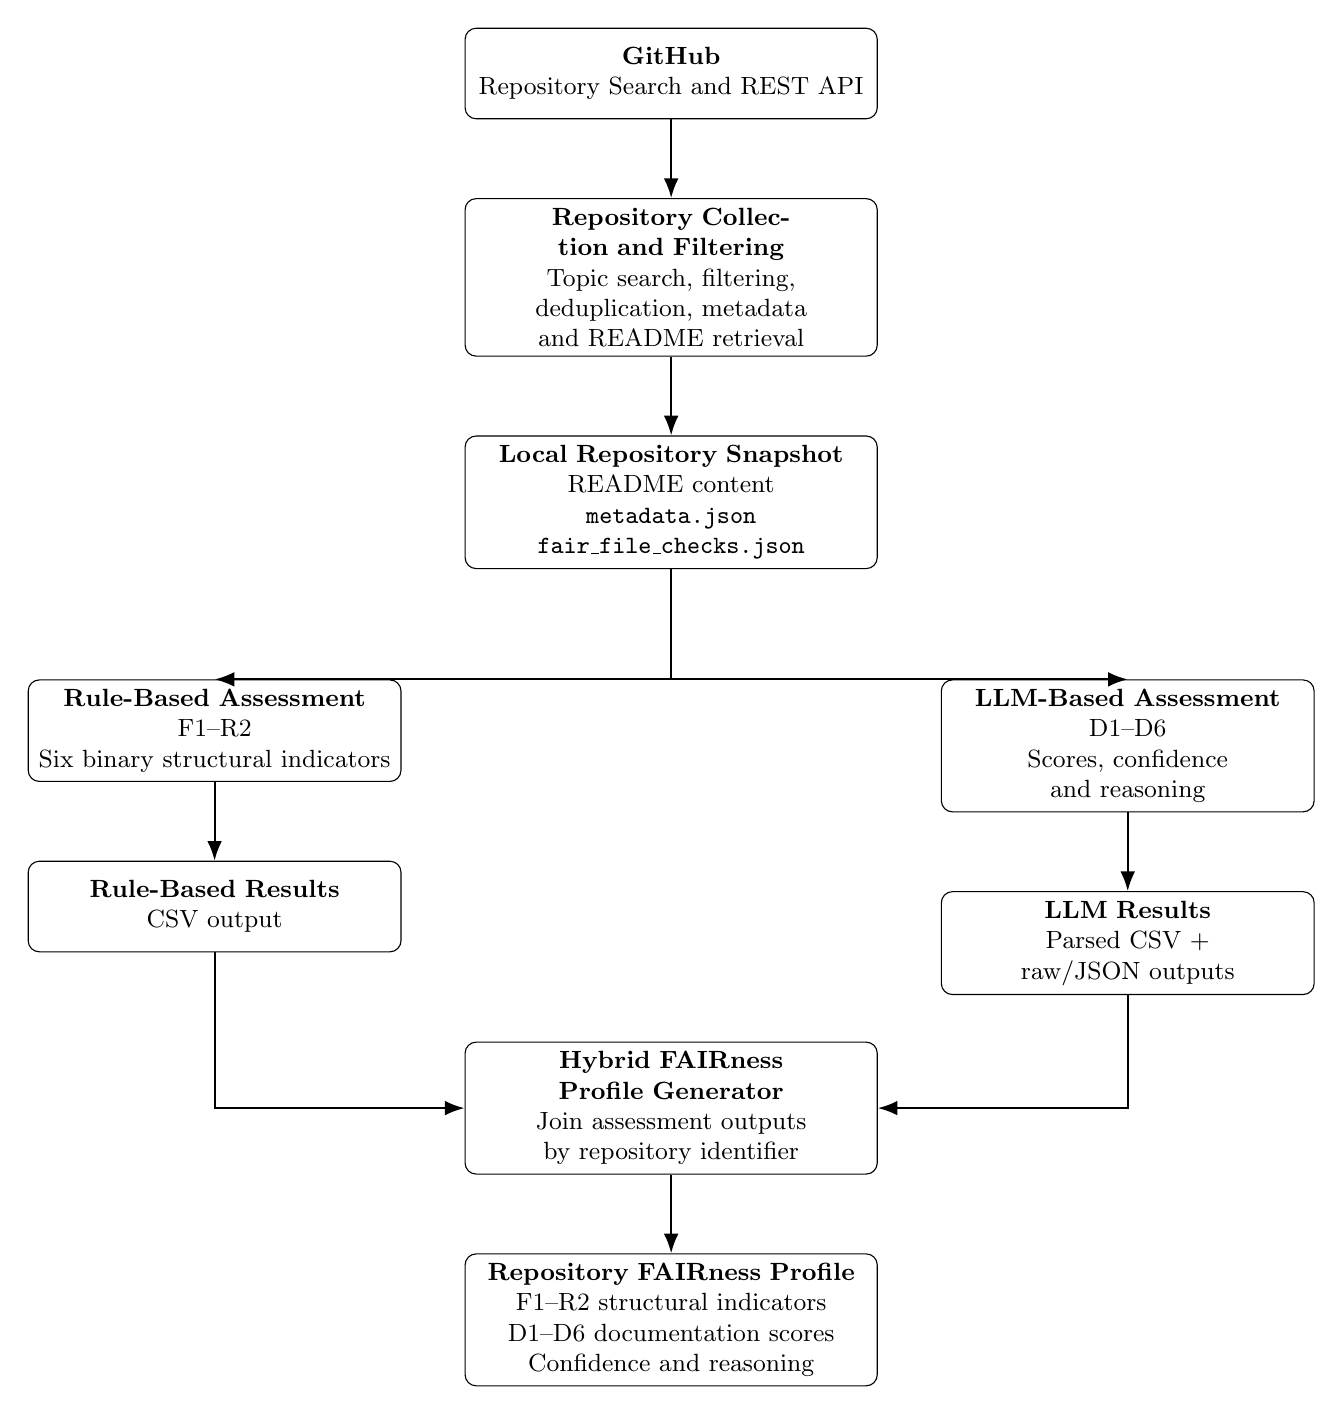
\begin{tikzpicture}[
    node distance=1.0cm and 1.2cm,
    box/.style={
        draw,
        rounded corners,
        rectangle,
        align=center,
        minimum height=1.15cm,
        text width=5.0cm,
        font=\small
    },
    smallbox/.style={
        draw,
        rounded corners,
        rectangle,
        align=center,
        minimum height=1.15cm,
        text width=4.5cm,
        font=\small
    },
    arrow/.style={
        -{Latex[length=2.5mm]},
        thick
    }
]

% GitHub
\node[box] (github) {
    \textbf{GitHub}\\
    Repository Search and REST API
};

% Collection
\node[box, below=of github] (collection) {
    \textbf{Repository Collection and Filtering}\\
    Topic search, filtering, deduplication,
    metadata and README retrieval
};

% Snapshot
\node[box, below=of collection] (snapshot) {
    \textbf{Local Repository Snapshot}\\
    README content\\
    \texttt{metadata.json}\\
    \texttt{fair\_file\_checks.json}
};

% Rule branch
\node[smallbox, below left=1.4cm and 0.8cm of snapshot] (rule) {
    \textbf{Rule-Based Assessment}\\
    F1--R2\\
    Six binary structural indicators
};

% LLM branch
\node[smallbox, below right=1.4cm and 0.8cm of snapshot] (llm) {
    \textbf{LLM-Based Assessment}\\
    D1--D6\\
    Scores, confidence and reasoning
};

% Rule output
\node[smallbox, below=of rule] (ruleout) {
    \textbf{Rule-Based Results}\\
    CSV output
};

% LLM output
\node[smallbox, below=of llm] (llmout) {
    \textbf{LLM Results}\\
    Parsed CSV + raw/JSON outputs
};

% Hybrid
\node[box, below=2.0cm of snapshot, yshift=-4.0cm] (hybrid) {
    \textbf{Hybrid FAIRness Profile Generator}\\
    Join assessment outputs by repository identifier
};

% Final profile
\node[box, below=of hybrid] (profile) {
    \textbf{Repository FAIRness Profile}\\
    F1--R2 structural indicators\\
    D1--D6 documentation scores\\
    Confidence and reasoning
};

% Arrows
\draw[arrow] (github) -- (collection);
\draw[arrow] (collection) -- (snapshot);

\draw[arrow] (snapshot.south) |- (rule.north);
\draw[arrow] (snapshot.south) |- (llm.north);

\draw[arrow] (rule) -- (ruleout);
\draw[arrow] (llm) -- (llmout);

\draw[arrow] (ruleout.south) |- (hybrid.west);
\draw[arrow] (llmout.south) |- (hybrid.east);

\draw[arrow] (hybrid) -- (profile);

\end{tikzpicture}
     \caption{Processing flow of the implemented hybrid FAIRness assessment pipeline.}
    \label{fig:system_architecture}
\end{figure}

First, the collection component retrieves and prepares repository
information from GitHub, producing the local repository snapshots used
as input to subsequent stages. Second, the rule-based component
evaluates structural evidence and produces six binary indicators
(F1--R2). Third, the LLM-based documentation component processes README documentation
and produces six ordinal documentation scores (D1--D6), each
accompanied by a confidence label and a short reasoning statement.
Finally, the hybrid profile generation component joins the structural
and documentation-based outputs by repository identifier and stores
them as a unified repository profile while preserving the two
assessment components as separate dimensions.

The rule-based assessment was executed for the complete
188-repository dataset. LLM assessment was executed for the
30-repository ground-truth corpus used for manual evaluation, and
hybrid profiles were consequently generated for repositories for
which both rule-based and LLM-based results were available. The implemented components therefore cover all stages required to
construct the hybrid profile, while the experimental execution of the
LLM-based component is restricted to the annotated evaluation corpus.

In addition to the batch-processing workflow used for the empirical
evaluation, the implemented framework provides a web-based interface
for inspecting saved assessment results and applying the assessment
procedure to a newly supplied public GitHub repository. The web layer
is implemented using FastAPI and a lightweight HTML, CSS, and
JavaScript frontend. It reuses the existing assessment components
rather than implementing a separate scoring procedure. Saved thesis
results and newly generated live assessments are kept distinct so that
interactive use of the prototype does not modify the fixed datasets
used for the empirical evaluation.

\section{Repository Data Collection and Local Representation}

Repository data collection is implemented as a two-phase process:
repository discovery and selection, followed by per-repository data
retrieval. Both phases interact with the GitHub REST API and are
implemented as separate Python components. Repository discovery
constructs the initial dataset, whereas the retrieval stage operates
on the resulting repository list to obtain the artefacts required by
the subsequent assessment components.

Repository discovery queries GitHub for repositories associated with
the research domains defined during dataset construction. Candidate
repositories are deduplicated by their GitHub repository identifier
and filtered according to the inclusion and exclusion criteria
described in Chapter~3. These criteria remove repositories that do not
meet the intended characteristics of the research software dataset,
including repositories identified as forks, archived projects, and
repositories matching predefined exclusion conditions. The resulting
repository list is persisted in machine-readable form and subsequently
processed by the data retrieval stage.

For each selected repository, the retrieval component obtains three
main types of information. First, README content is retrieved through
GitHub's dedicated README endpoint and stored locally for subsequent
documentation assessment. Second, the repository metadata returned by
the GitHub repository endpoint is stored in a \texttt{metadata.json}
file. This record contains the GitHub metadata required by later
processing stages, including repository and licensing information.
Third, the contents of the repository root are queried and compared
against a predefined set of FAIR-related filenames. The resulting
presence inventory is stored as
\texttt{fair\_file\_checks.json}. Candidate files include README and
license variants, citation and structured metadata files, dependency
specifications, and contribution files.

The collected artefacts are organized as local repository snapshots.
Each repository is assigned a directory based on its owner and
repository name, containing the retrieved README, repository metadata,
and FAIR-related file inventory. This representation decouples data
collection from assessment: once a snapshot has been created, the
rule-based and LLM-based components can operate on the locally stored
evidence without repeatedly querying GitHub. It also makes the exact
repository evidence used during an assessment directly inspectable.

The full-dataset retrieval implementation includes basic support for
resuming interrupted collection runs. Before retrieving a repository,
the collector checks whether a local \texttt{metadata.json} file
already exists and, if so, skips that repository. This avoids repeated
API requests for repositories treated as previously collected, although
the presence of this file is used as the completion marker and the
collector does not independently verify that every expected snapshot
artefact is present. The ground-truth collection workflow does not use
the same repository-level skip mechanism. The resulting snapshots form
the common input representation used by the subsequent assessment
components.

\section{Rule-Based Assessment Implementation}

The rule-based assessment component evaluates each repository
snapshot against the six binary FAIR indicators (F1--R2) defined in
Chapter~3, operating exclusively on the locally stored README,
metadata, and file-inventory artefacts produced by the collection
stage; no GitHub API access occurs during scoring.

Each indicator is implemented as an independent boolean check,
drawing on one or more of three evidence sources: the precomputed
file-presence inventory, the stored GitHub metadata record, and the
README text itself. F2 (Structured Metadata) is evaluated by
checking for recognized metadata filenames using both the stored
file-presence inventory and the local repository snapshot. R1
(README Present) directly checks the snapshot for one of the
recognized README filename variants. I1 (Dependency Specification)
similarly evaluates recognized dependency and build files across
multiple programming-language ecosystems. F1 (Persistent Identifier)
searches the README together with any locally stored
\texttt{CITATION.cff} and \texttt{codemeta.json} content for patterns
associated with common persistent identifier formats, including
doi.org URLs, Zenodo record and badge links, and Software Heritage
identifiers. A1 (License) reflects the three evidence sources
described in Chapter~3: a recognized license filename, a license
field in the stored GitHub metadata, or explicit licensing language
in the README text; the three sources are checked in this order, so
that structured evidence takes precedence and README text is only
relied upon when no file or metadata evidence is found. R2 (Citation
Information) is satisfied either by the presence of a dedicated
citation file or by matching one of several phrasings commonly used
to request citation of a software project within the README text.

Where file-presence evidence is required, the implementation does
not rely solely on the precomputed inventory. The corresponding path
in the local repository snapshot is also checked, allowing a
file-based indicator to be satisfied when the artefact exists locally
but is absent from the stored presence record.

The scorer processes repositories in batch, reading each
repository's snapshot folder in turn and producing a single
six-indicator vector per repository, together with an aggregated
rule-based total ranging from 0 to 6. Repositories whose snapshot is
incomplete --- for example, missing the metadata or file-inventory
record --- are skipped and reported rather than scored with
incomplete evidence. Results are written to a single CSV file, with
one row per repository, in which each of the six indicators and the
aggregated total form separate columns. This output format is shared
by both the full 188-repository dataset run and the 30-repository
ground truth validation run.


\section{LLM-Based Assessment Implementation}
The LLM-based assessment component evaluates README documentation
against the six documentation quality dimensions (D1--D6) defined in
Chapter~3. Two model configurations are supported: Llama~3.1~8B
through a locally running Ollama instance and
\texttt{Qwen3.6-35B-A3B-MLX-8bit} through the university KISTE
service using an OpenAI-compatible API.

The two implementations share the same substantive assessment rubric,
README-only evidence boundary, and 12,000-character input limit, while
provider-specific request and response handling is implemented
separately.

For each repository, the README is located by checking a fixed set
of recognized filenames in priority order, so that non-Markdown
README variants are still picked up if present. The retrieved text
is truncated to the first 12{,}000 characters where it exceeds this
length, consistent with the preprocessing limit described in
Chapter~3, before being inserted into a fixed prompt template
together with the repository name. The prompt instructs the model to score each of the six dimensions
according to the rubric criteria and to base each score only on evidence
explicitly present in the README text. Both model configurations return
a score, confidence label (HIGH, MEDIUM, or LOW), and reasoning field
for each dimension. The Qwen prompt additionally requests a concise
one-sentence justification, while the Llama implementation requires the
reasoning field through its structured response schema.

For the primary Llama~3.1~8B configuration, the scorer submits each
request to Ollama's HTTP API rather than invoking the model through a
command-line interface. The sampling temperature is set to zero, and a
structured JSON schema is supplied as part of the request. The schema
constrains the response to the six required dimensions, restricts each
score to the integer values 0, 1, or 2, and restricts each confidence
label to one of the three permitted values.

On receiving a response, the Llama implementation performs an
additional validation pass independent of the schema, confirming that
all six dimensions are present and that every score and confidence
value falls within the expected range before accepting the result. If
a response is missing, malformed, or fails this validation, the request
is retried once; if the retry also fails, the repository is recorded
as failed and scoring proceeds to the next repository rather than
halting the batch run.

Nonempty raw model responses are persisted before parsing, preserving
the original output returned by the model service for later inspection,
including responses that subsequently fail parsing or validation.
Attempts that return no response, or fail before a model response is
received, do not produce a raw-response file. For successfully scored
repositories, the parsed and validated JSON representation is stored
separately.

Batch execution is resumable at the level of individual repositories.
Before submitting a repository for assessment, the implementation
checks whether a previously parsed result is already available and
skips repositories that have already been successfully processed.
This allows interrupted runs to continue without repeating completed
LLM inference.

Successfully scored repositories are appended incrementally to a
single CSV output file as they complete, with one row per repository
containing the score, confidence level, and reasoning text for each
of the six dimensions, together with the model name and a timestamp.
This output format matches the one described in Chapter~3 and is
applied to all 30 ground truth repositories.

A second LLM-based scorer implementation targets Qwen3.6-35B-A3B-MLX-8bit, 
accessed through an OpenAI-compatible chat completion API hosted on a remote 
GPU server rather than through the local Ollama instance. This implementation 
reuses the same dimension definitions, substantive prompt structure, and rubric described above, 
adapted only where required by the different backend: structured output is obtained 
through explicit prompt instructions combined with post-hoc JSON validation rather than 
a server-enforced schema, and the model's separately returned reasoning trace is discarded 
before scoring. Results are written to per-model output files following the same schema as the 
Llama-based output, so that the two models' results can be compared directly without either overwriting 
the other.
 \section{Hybrid Profile Generation}

The hybrid profile generation component combines the outputs of the
rule-based and LLM-based components into a single unified record per
repository, without computing any combined or weighted score.

The component reads the rule-based and LLM-based result CSV files
produced by the two preceding stages and indexes each by repository
identifier. This process is repeated independently for each evaluated 
LLM configuration, producing one hybrid profile set per model, each 
generated by joining the shared rule-based results with that model's 
LLM-based results. An inner join is then performed between the two sets of
results, so that a hybrid profile is produced only for repositories
present in both inputs. Because the LLM-based component was applied
only to the 30-repository ground truth corpus, this join
consequently restricts the set of generated hybrid profiles to those
repositories, even though rule-based results exist for the complete
188-repository dataset.

For each matched repository, the resulting record concatenates the
six rule-based indicator scores (F1--R2) and the aggregated
rule-based total with the six LLM-based dimension scores (D1--D6),
each accompanied by its confidence level and reasoning text, the
aggregated LLM total, and the model name and timestamp associated
with the LLM assessment. No arithmetic combination or weighting is
applied across the two sets of scores at any point in this process;
the structural and documentation-based dimensions are retained as
distinct fields within the same record, consistent with the design
rationale described in Chapter~3. A single timestamp is recorded for
the batch as a whole, and repositories are written in a fixed,
sorted order to ensure that the output is deterministic regardless
of the order in which the two input files were produced.

The combined records are written to a single CSV file, with one row
per repository, representing the hybrid FAIRness profile produced by
the proposed framework. The profile provides a unified representation
of the structural and documentation-based assessment results while
preserving their distinct scoring schemes.

\section{Example Repository Profile}

To illustrate the output produced by the framework, this section
presents the complete hybrid FAIRness profile generated for
\texttt{astropy/astropy}, one of the 30 ground truth repositories.
This repository was selected because its profile shows a clear
contrast between the two assessment components: it achieves the
maximum possible rule-based score while receiving a comparatively
low LLM-based documentation score, illustrating the kind of gap
that a purely structural assessment would not reveal.

\subsection{Rule-Based Indicators}

Table~\ref{tab:example_rule} shows the six rule-based indicator
scores produced for this repository.

\begin{table}[h]
\centering
\caption{Rule-based indicator scores for \texttt{astropy/astropy}.}
\label{tab:example_rule}
\begin{tabular}{lc}
\hline
\textbf{Indicator} & \textbf{Score} \\
\hline
F1 --- Persistent Identifier    & 1 \\
F2 --- Structured Metadata      & 1 \\
A1 --- License                  & 1 \\
I1 --- Dependency Specification & 1 \\
R1 --- README Present           & 1 \\
R2 --- Citation Information     & 1 \\
\hline
\textbf{Rule-based total}       & \textbf{6 / 6} \\
\hline
\end{tabular}
\end{table}

The repository satisfies all six structural indicators, reflecting
the presence of a persistent identifier, a structured metadata file,
a recognized license, a dependency specification file, a README, and
explicit citation information.

It is important to note that this assessment is restricted to evidence
contained directly in the README. The Astropy README links to extensive
external documentation that provides additional installation, usage,
and dependency information; however, the content behind these links is
not retrieved by the implemented LLM assessment pipeline. Consequently,
the scores in Table~\ref{tab:example_llm} should be interpreted as an
assessment of the documentation evidence available directly in the
README, rather than of the overall quality or completeness of Astropy's
documentation.

\subsection{LLM-Based Documentation Dimensions}
Table~\ref{tab:example_llm} shows the documentation-quality assessment
produced by the primary Llama~3.1~8B configuration for
\texttt{astropy/astropy}, together with the confidence level and
reasoning associated with each dimension.
\begin{table}[h]
\centering
\caption{Llama~3.1~8B documentation assessment for
\texttt{astropy/astropy}.}
\label{tab:example_llm}
\small
\begin{tabular}{lccp{8cm}}
\hline
\textbf{Dimension} & \textbf{Score} & \textbf{Confidence} & \textbf{Reasoning} \\
\hline

D1 --- Installation
  & 0
  & HIGH
  & The README provides only a single line of installation
    information (\texttt{pip install astropy}), without mentioning
    required prerequisites. \\

D2 --- Usage
  & 0
  & HIGH
  & There is no concrete command, code snippet, workflow, or
    executable example in the README to demonstrate how to use the
    software. \\

D3 --- Purpose
  & 1
  & MEDIUM
  & The README explains that Astropy is a community effort to
    develop a single core package for astronomy in Python, but it
    does not clearly explain its intended domain or audience. \\

D4 --- Dependencies
  & 0
  & HIGH
  & There is no information about required and/or optional
    dependencies provided in human-readable form in the README. \\

D5 --- Examples
  & 1
  & MEDIUM
  & The README mentions GitHub Codespaces as a way to start
    developing Astropy, but it does not contain a meaningful usage
    example, nor explicitly link to an example gallery or tutorial
    demonstrating software use. \\

D6 --- Contribution
  & 2
  & HIGH
  & The README provides contribution guidance and at least one
    support or community channel (Slack), as well as multiple ways
    to contribute, including code submission, feedback, and
    documentation updates. \\
\hline
\multicolumn{3}{l}{\textbf{LLM total}} & \textbf{4 / 12} \\
\hline
\end{tabular}
\end{table}

The confidence label reflects the model's self-reported confidence in
the assigned score itself, independent of whether that score is low or
high: a HIGH label on D1 indicates high confidence in assigning a low
score because installation information is lacking, just as the HIGH
label on D6 indicates high confidence in assigning a high score because
the contribution guidance is present and complete.

\subsection{Profile Representation}

The example illustrates how the implemented hybrid profile preserves
the outputs of the two assessment components separately. The
rule-based component assigns positive values to all six implemented
structural indicators, resulting in a total of 6/6. The Llama-based
component produces a documentation total of 4/12, together with
dimension-specific scores, confidence labels, and reasoning.

These documentation values represent the output generated by the
implemented LLM assessment pipeline rather than independently validated
judgements of documentation quality. In particular, the profile
preserves the model's original criterion-level decisions even where
their correspondence with the annotation rubric requires further
evaluation.

The example therefore demonstrates the representation produced by the
hybrid implementation: structural evidence and LLM-based documentation
assessment are available for the same repository without being
collapsed into a single overall FAIRness score. The correctness and
reliability of these outputs relative to the manual annotations are
evaluated separately in Chapter~5.

\section{Web-Based Assessment Interface}

\subsection{Web Application Architecture}

To make the assessment results inspectable and to demonstrate the
framework beyond batch-generated CSV files, a web-based prototype was
implemented on top of the assessment pipeline. The application uses a
FastAPI backend together with a lightweight frontend implemented in
HTML, CSS, and JavaScript.

The web layer does not introduce an alternative assessment procedure.
Instead, it reuses the same rule-based and LLM-based scoring logic used
by the batch-processing pipeline. The backend provides access to the
saved thesis results and coordinates live repository assessment, while
the frontend presents the resulting structural and documentation-based evidence in an interactive form.

The application distinguishes between two result sources. Saved thesis
assessments correspond to the fixed datasets used in the empirical
study, whereas live assessments are generated from the current content
of a user-supplied public GitHub repository. Live assessments are not
written into the fixed thesis dataset and therefore do not alter the
results evaluated in Chapter~5.

\subsection{Dataset Overview}

The overview view provides an aggregate representation of the saved
assessment results. Structural evidence is summarized across the full
dataset of 188 repositories, while documentation-quality results are
reported for the 30-repository annotated corpus on which the LLM-based
assessment was executed. The interface explicitly distinguishes these
two populations to avoid implying that documentation scores are
available for all 188 repositories.

Because documentation assessments were generated separately for the
two evaluated LLM configurations, the interface allows the displayed
saved documentation results to be selected by model. Changing this
selection affects the documentation summaries and repository-level
documentation results, while the deterministic structural assessment
remains unchanged. Model selection is exposed primarily to support
transparent inspection of model-dependent assessment behaviour rather
than to imply that the two configurations are interchangeable.

The overview reports the prevalence of the six structural indicators,
the distribution of structural totals, and the mean scores of the six
README documentation dimensions for the selected model configuration.
Structural and documentation results remain visually separated and are
not combined into an overall FAIRness score, following the
hybrid-profile design described in Chapter~3.

Figure~\ref{fig:web_overview} shows the resulting dataset overview for
the two evaluated documentation model configurations.

\begin{figure}[p]
    \centering

    \begin{subfigure}{\textwidth}
        \centering
        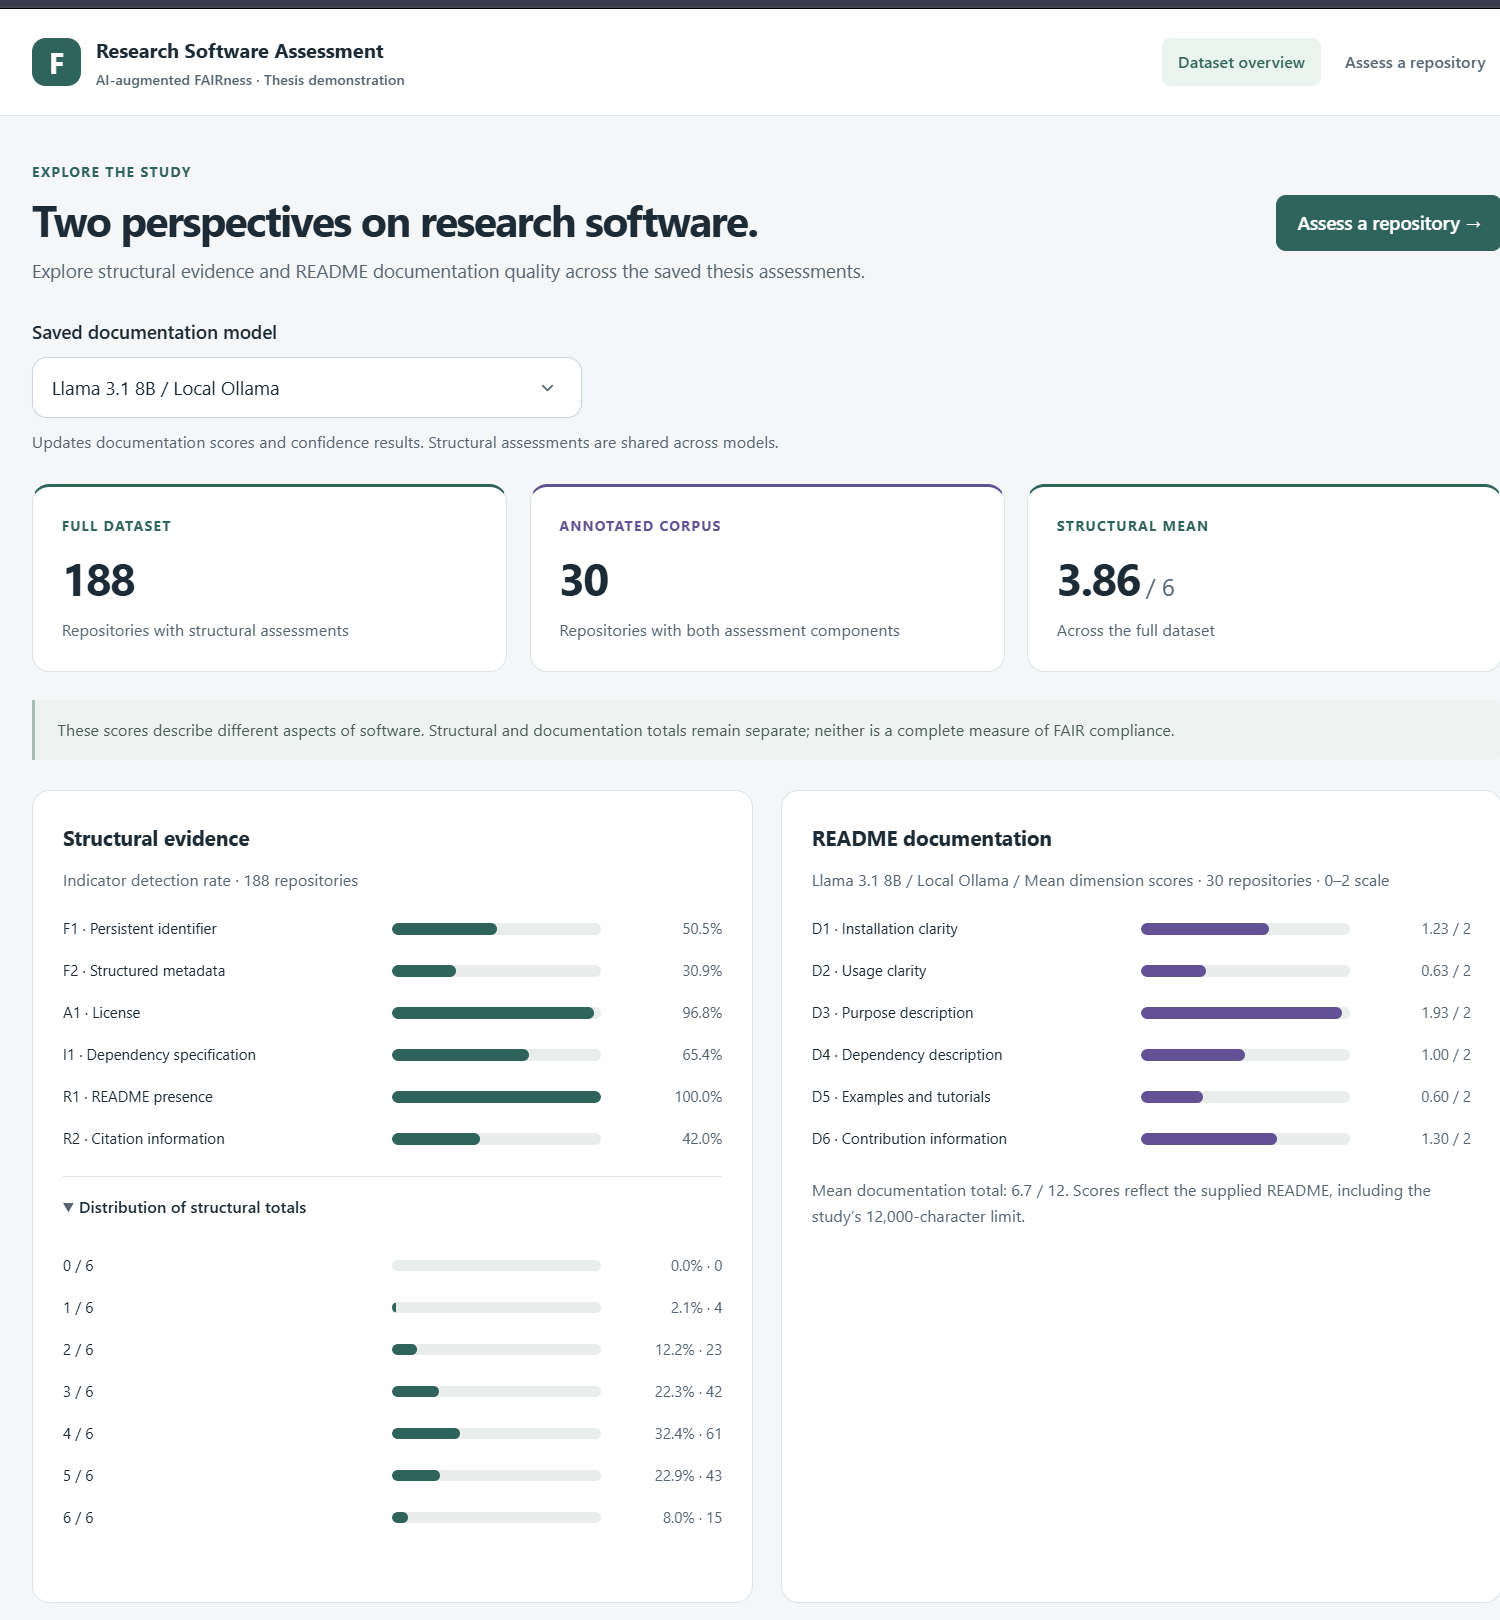
\includegraphics[
            width=\textwidth,
            height=0.36\textheight,
            keepaspectratio
        ]{figures/ui/web_overview_llama.png}
        \caption{Dataset overview with the saved Llama 3.1 8B assessment.}
        \label{fig:web_overview_llama}
    \end{subfigure}

    \vspace{0.7em}

    \begin{subfigure}{\textwidth}
        \centering
        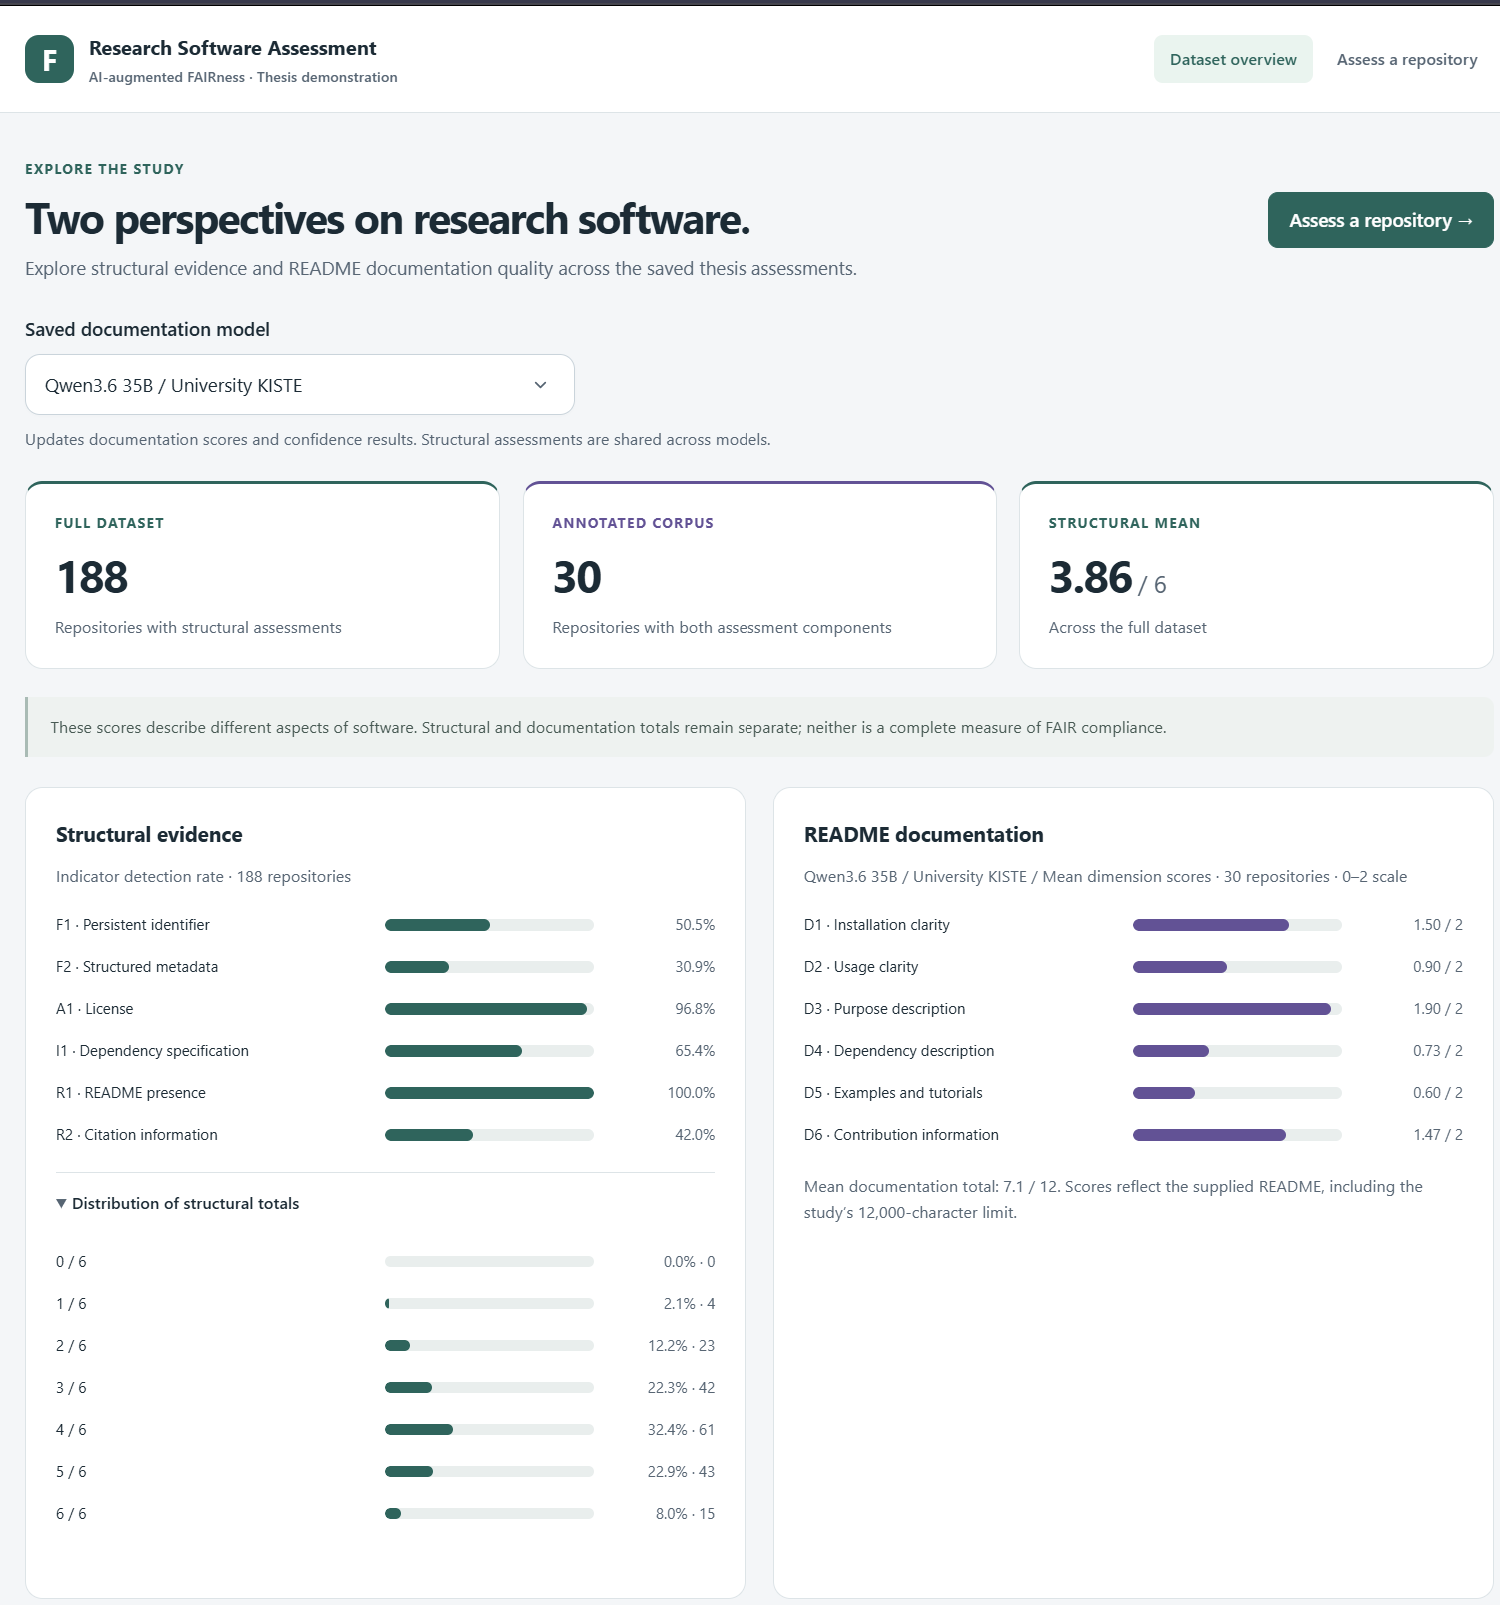
\includegraphics[
            width=\textwidth,
            height=0.36\textheight,
            keepaspectratio
        ]{figures/ui/web_overview_qwen.png}
        \caption{Dataset overview with the saved Qwen assessment.}
        \label{fig:web_overview_qwen}
    \end{subfigure}

    \caption{Dataset overview of the web-based assessment interface for
    the two evaluated documentation models. Structural evidence is shared
    across model selections, while the README documentation summaries
    reflect the selected LLM configuration.}
    \label{fig:web_overview}
\end{figure}

\FloatBarrier

\subsection{Research Evaluation View}

The web interface exposes selected evaluation results used to assess
the reliability of the implemented framework. The evaluation view
separates validation of the deterministic structural component from
analysis of the LLM-based documentation component.

For the structural component, precision, recall, and F1-score are
presented for each of the six binary indicators against the manually
annotated 30-repository corpus. The interface additionally reports the
corresponding results for the 20-repository pilot-exclusion subset.
This latter analysis is explicitly identified as an internal
consistency check rather than as independent validation, since some
annotations in this subset were corrected during scorer validation
using the finalized rubric.

For the documentation component, the interface provides two forms of
evaluation information. First, model-reported confidence labels are
shown together with exact agreement, mean absolute error, and weighted
Cohen's Kappa against the human reference annotations. The interface
explicitly states that these confidence labels are self-reported and
should not be interpreted as calibrated probabilities of correctness.

Second, an interactive agreement view allows the two evaluated LLM
configurations to be compared against either the primary or second
human annotator. The user can inspect results for the complete
30-repository annotated corpus or exclude the ten pilot repositories
to obtain the 20-repository pilot-exclusion sensitivity analysis.
For each model, the interface reports mean weighted Cohen's Kappa,
exact agreement, and mean absolute error, together with corresponding
per-dimension results for D1--D6. Higher documentation scores are not
presented as evidence of better model performance; agreement is
evaluated relative to the selected human reference.

Figures~\ref{fig:web_evaluation_validation} and
\ref{fig:web_evaluation_agreement} illustrate these two parts of the
research evaluation interface. The methodology and interpretation of
the displayed results are discussed in Chapter~5.

\begin{figure}[p]
    \centering
    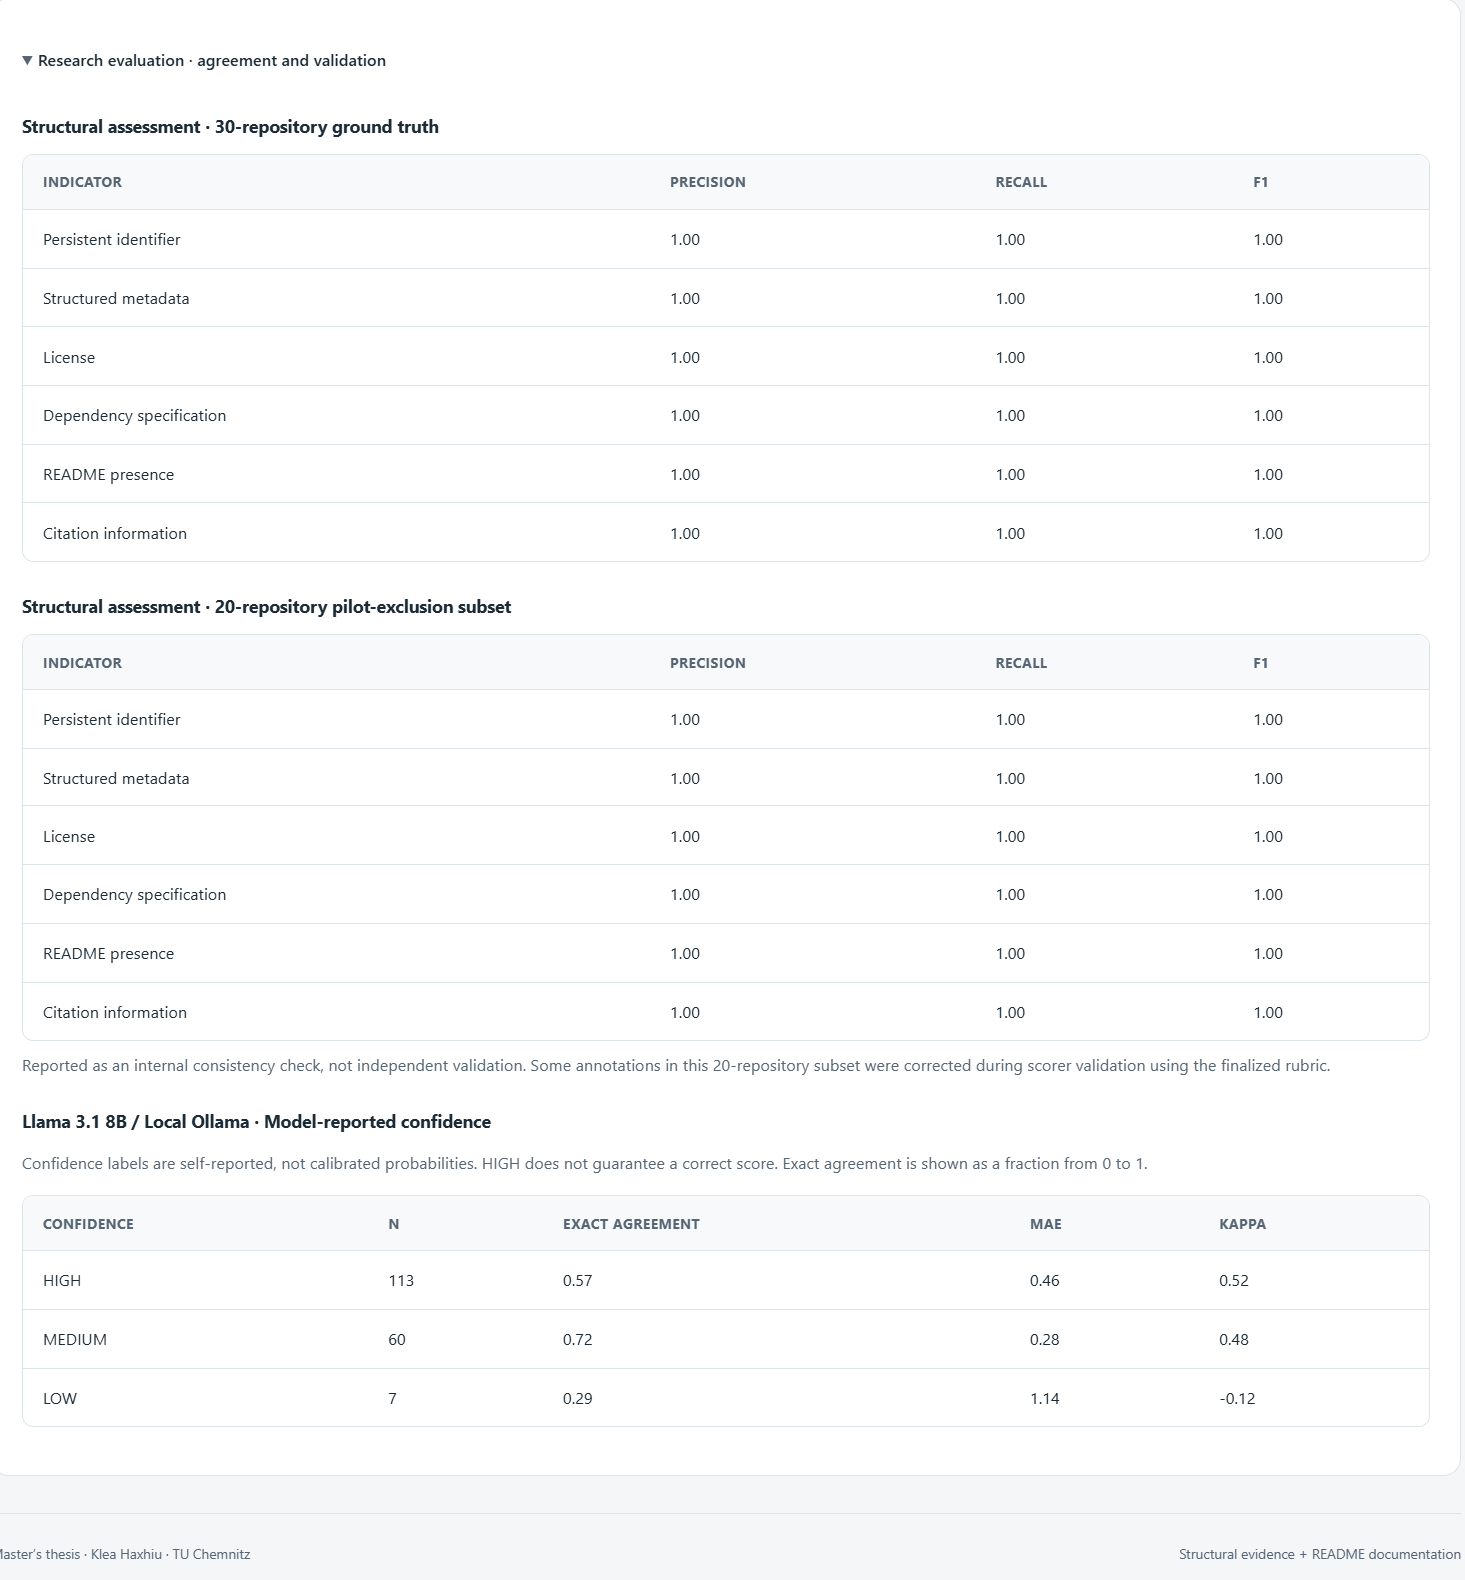
\includegraphics[
        width=\textwidth,
        height=0.78\textheight,
        keepaspectratio
    ]{figures/ui/web_structural_validation_confidence.png}
    \caption{Structural validation and confidence analysis in the
    research evaluation interface. The view reports precision, recall,
    and F1-score for the structural indicators on the annotated corpus
    and pilot-exclusion subset, together with model-reported confidence
    statistics for the documentation assessment.}
    \label{fig:web_evaluation_validation}
\end{figure}

\begin{figure}[p]
    \centering
    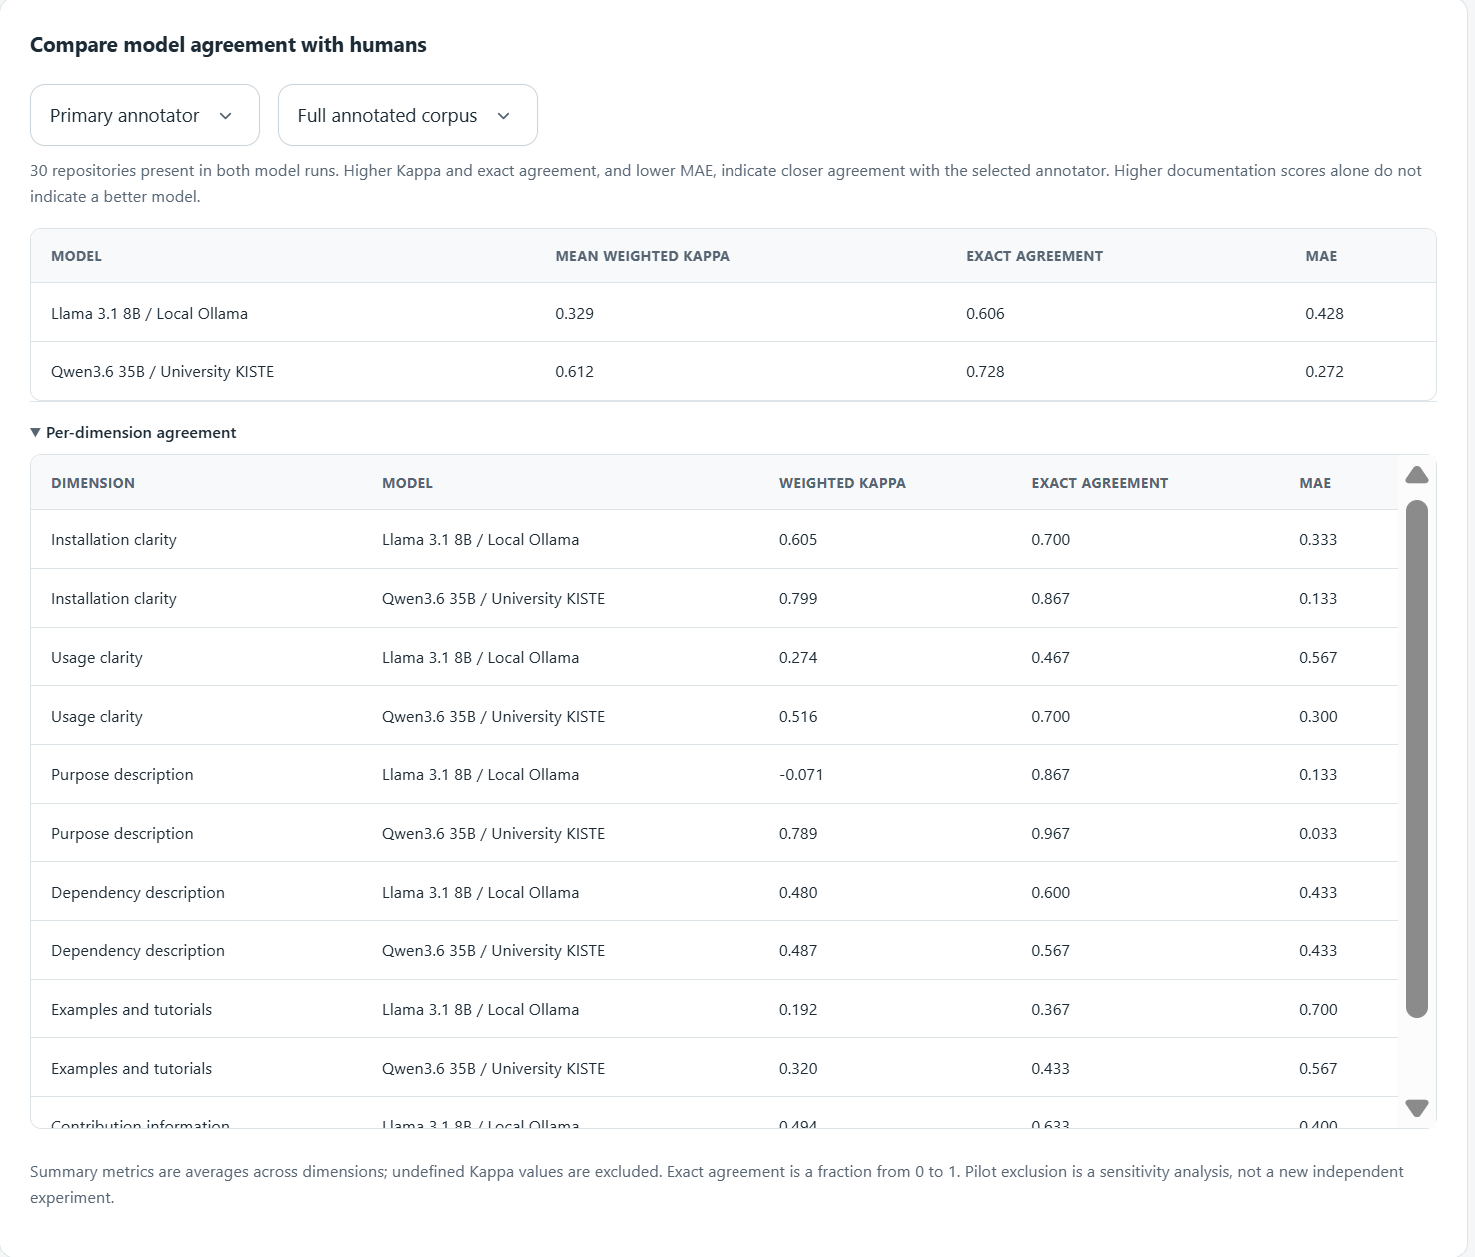
\includegraphics[
        width=\textwidth,
        height=0.78\textheight,
        keepaspectratio
    ]{figures/ui/web_evaluation_agreement.png}
    \caption{LLM--human agreement view for the annotated corpus. The
    interface compares the saved Llama and Qwen assessments against
    the selected human annotator using weighted Cohen's Kappa, exact
    agreement, and mean absolute error, with corresponding
    per-dimension results for D1--D6.}
    \label{fig:web_evaluation_agreement}
\end{figure}

\FloatBarrier


\subsection{Model Comparison View}

For repositories in the annotated evaluation corpus, the prototype
provides a side-by-side comparison of the saved Llama and Qwen
documentation assessments. The comparison presents the D1--D6 scores
from both model configurations together with the selected human
reference annotations and highlights dimensions on which the model
outputs differ.

This functionality is intended primarily to support transparent
inspection of model-dependent assessment behaviour rather than to
present the two configurations as interchangeable user preferences.
The comparison operates exclusively on the saved experimental results
and does not trigger new LLM inference. Model identifiers, reasoning
statements, and confidence labels remain visible so that differences
can be traced to the corresponding assessment output.

Figure~\ref{fig:web_model_comparison} shows the model-comparison view
for a repository from the annotated corpus.

\begin{figure}[p]
    \centering
    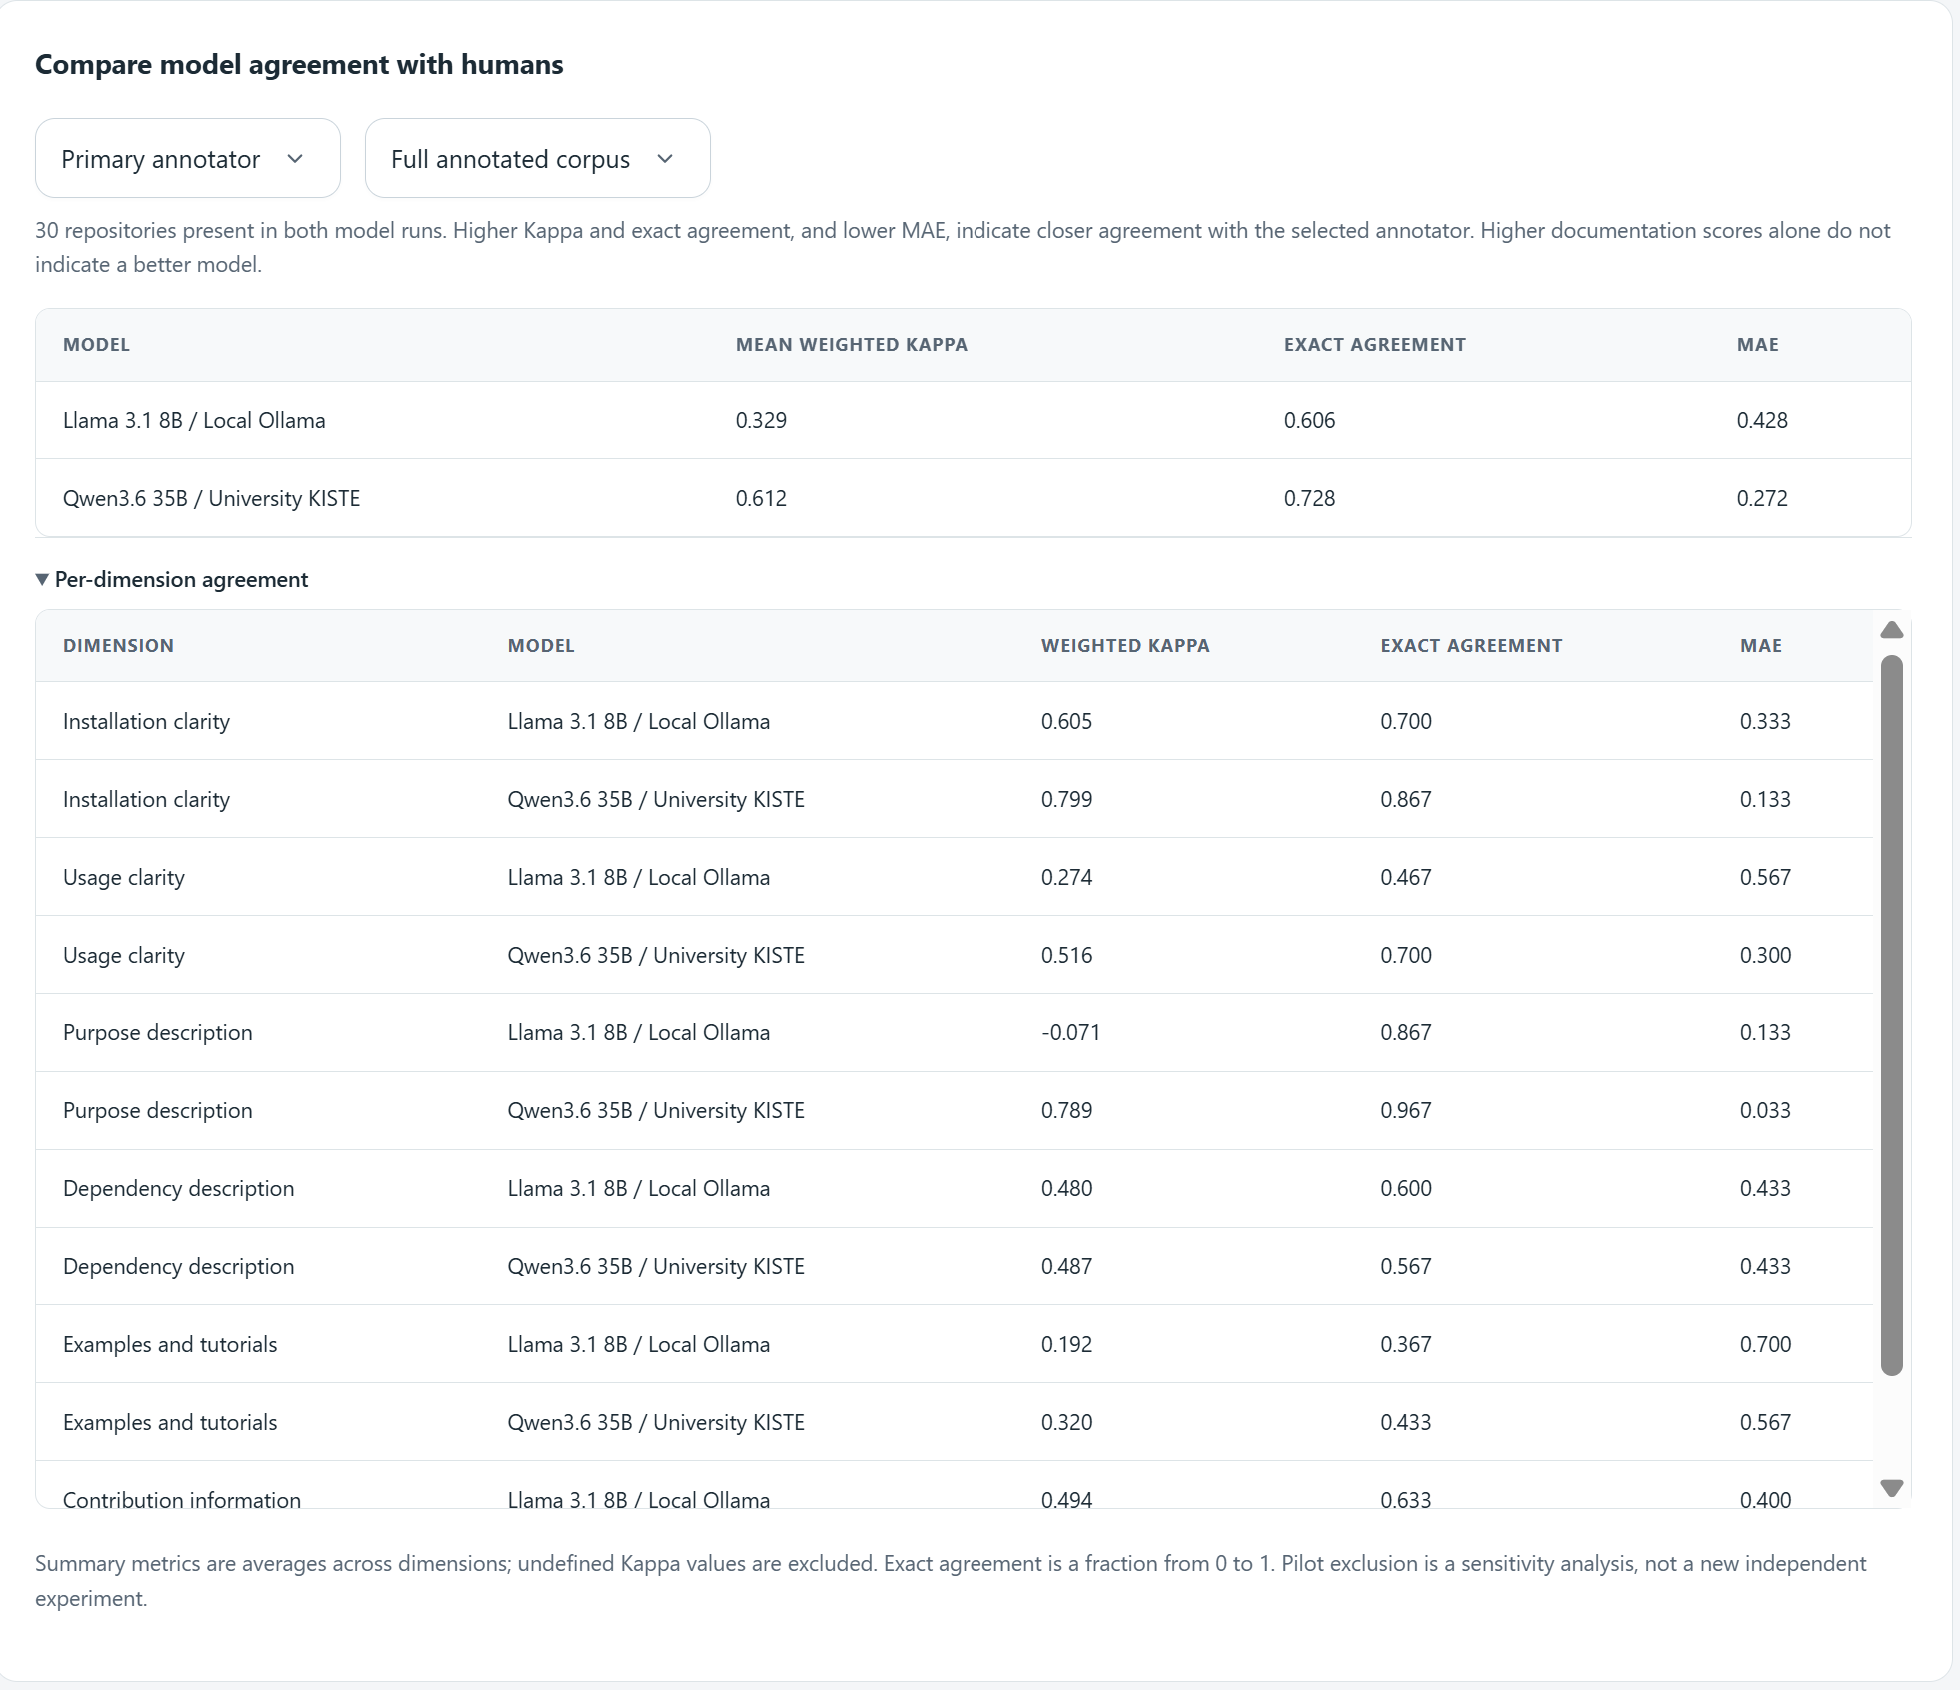
\includegraphics[
        width=\textwidth,
        height=0.78\textheight,
        keepaspectratio
    ]{figures/ui/web_model_comparison.png}
    \caption{Model-comparison view for a repository in the annotated
    corpus. Saved Llama and Qwen documentation assessments are shown
    alongside the selected human reference scores, allowing
    model-dependent differences across D1--D6 to be inspected.}
    \label{fig:web_model_comparison}
\end{figure}

\FloatBarrier

\subsection{Repository Browser}

The web interface includes a searchable repository browser that
provides access to the saved assessment results. Users can search by
repository owner or name and switch between the annotated corpus and
the full repository dataset.

For the annotated corpus, the browser contains the 30 repositories for
which both structural and LLM-based documentation assessments are
available. The documentation totals shown in this view correspond to
the currently selected LLM configuration, while the structural results
remain unchanged because they are independent of the selected model.
Repository entries provide access to the corresponding model-specific
saved report and, where both model outputs are available, to the
model-comparison view.

In contrast, the full-dataset view contains all 188 repositories for
which the structural assessment was executed. Since the LLM-based
assessment was not executed across this complete dataset, the
documentation field is shown as ``Not assessed'' rather than assigning
a documentation score of zero.

Selecting ``View report'' opens the repository-level assessment view,
where the individual structural indicators and, where available,
documentation dimensions and supporting assessment information can be
inspected. An example of this detailed view is presented in the
following subsection using \texttt{astropy/astropy}.

Figure~\ref{fig:web_repository_browser} shows the two repository-browser
cohorts exposed by the interface. The annotated-corpus view provides
access to the hybrid profiles for the 30 repositories with both
assessment components, whereas the full-dataset view exposes the
structural assessments for all 188 repositories and explicitly marks
documentation as not assessed where no LLM assessment was performed.

\begin{figure}[p]
    \centering

    \begin{subfigure}{\textwidth}
        \centering
        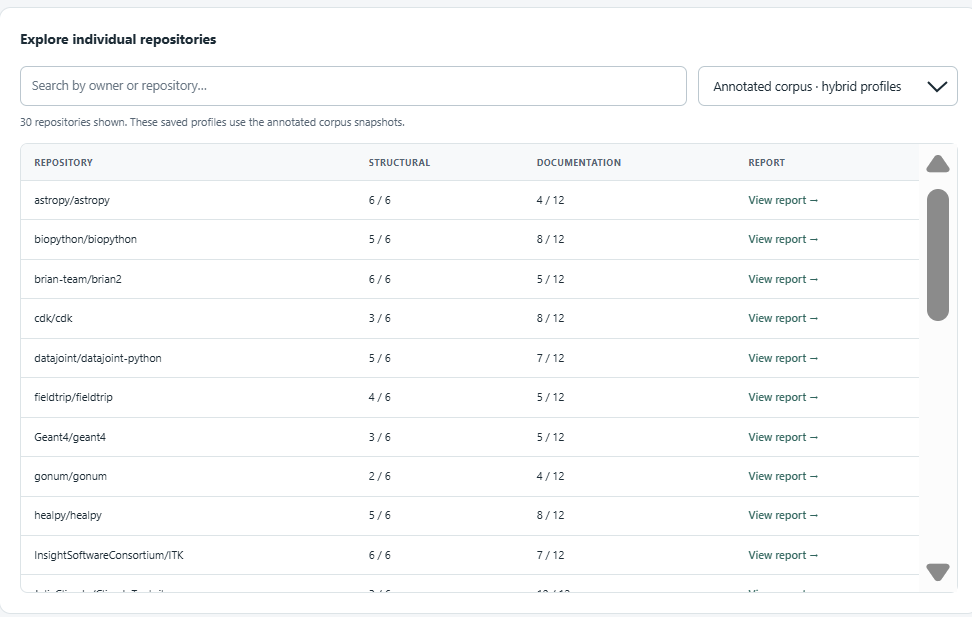
\includegraphics[
            width=\textwidth,
            height=0.36\textheight,
            keepaspectratio
        ]{figures/ui/web_browser_annotated.png}
        \caption{Annotated corpus with hybrid profiles.}
        \label{fig:web_browser_annotated}
    \end{subfigure}

    \vspace{0.7em}

    \begin{subfigure}{\textwidth}
        \centering
        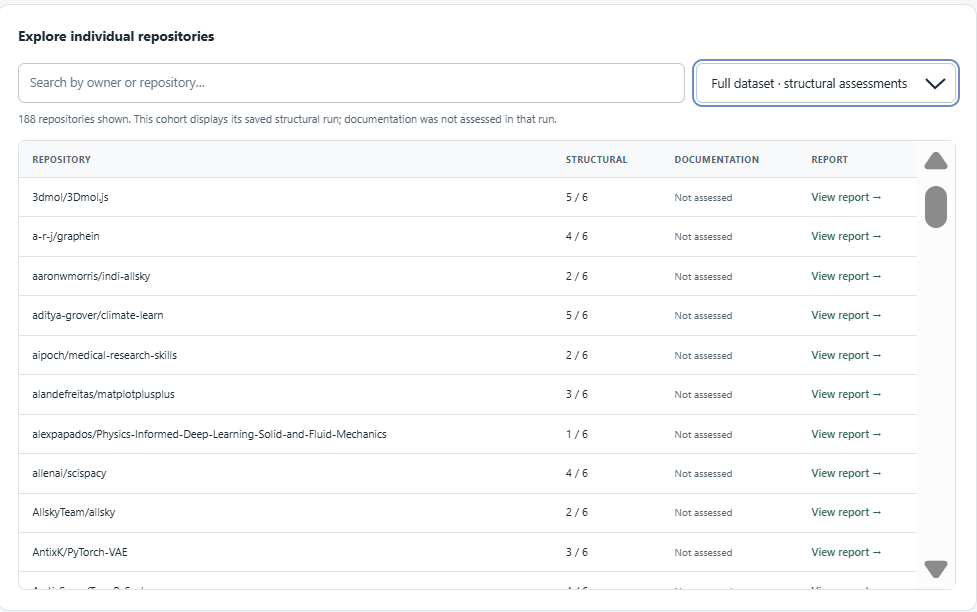
\includegraphics[
            width=\textwidth,
            height=0.36\textheight,
            keepaspectratio
        ]{figures/ui/web_browser_full.png}
        \caption{Full dataset with structural assessments only.}
        \label{fig:web_browser_full}
    \end{subfigure}

    \caption{Repository browser for the two saved assessment cohorts.
    (a) The 30-repository annotated corpus exposes structural and
    model-specific documentation results together with access to model
    comparison. (b) The full 188-repository dataset exposes the saved
    structural assessments, while documentation is marked as not assessed
    because LLM-based assessment was not executed for this cohort.}
    \label{fig:web_repository_browser}
\end{figure}

\FloatBarrier
\subsection{Repository-Level Assessment View}

Individual saved assessments can also be inspected through a
repository-level view. This view presents the six structural indicators
and six documentation dimensions as separate components of the hybrid
profile. Documentation dimensions can be expanded to inspect the
reasoning produced by the LLM, its model-reported confidence label, and
the rubric associated with the corresponding score.

Saved documentation assessments are model-specific. Selecting a
different LLM configuration loads the corresponding persisted
documentation scores, reasoning, confidence labels, and assessment
metadata, while the deterministic structural component remains
unchanged.

The interface additionally exposes the README evidence and assessment
metadata, including the result source, model, and assessment timestamp.
This provides a transparent presentation of the evidence underlying an
assessment rather than exposing only the resulting numerical scores.

Figure~\ref{fig:web_repository} shows the saved assessment for
\texttt{astropy/astropy}, corresponding to the example profile
presented in the preceding section.

\begin{figure}[p]
    \centering
    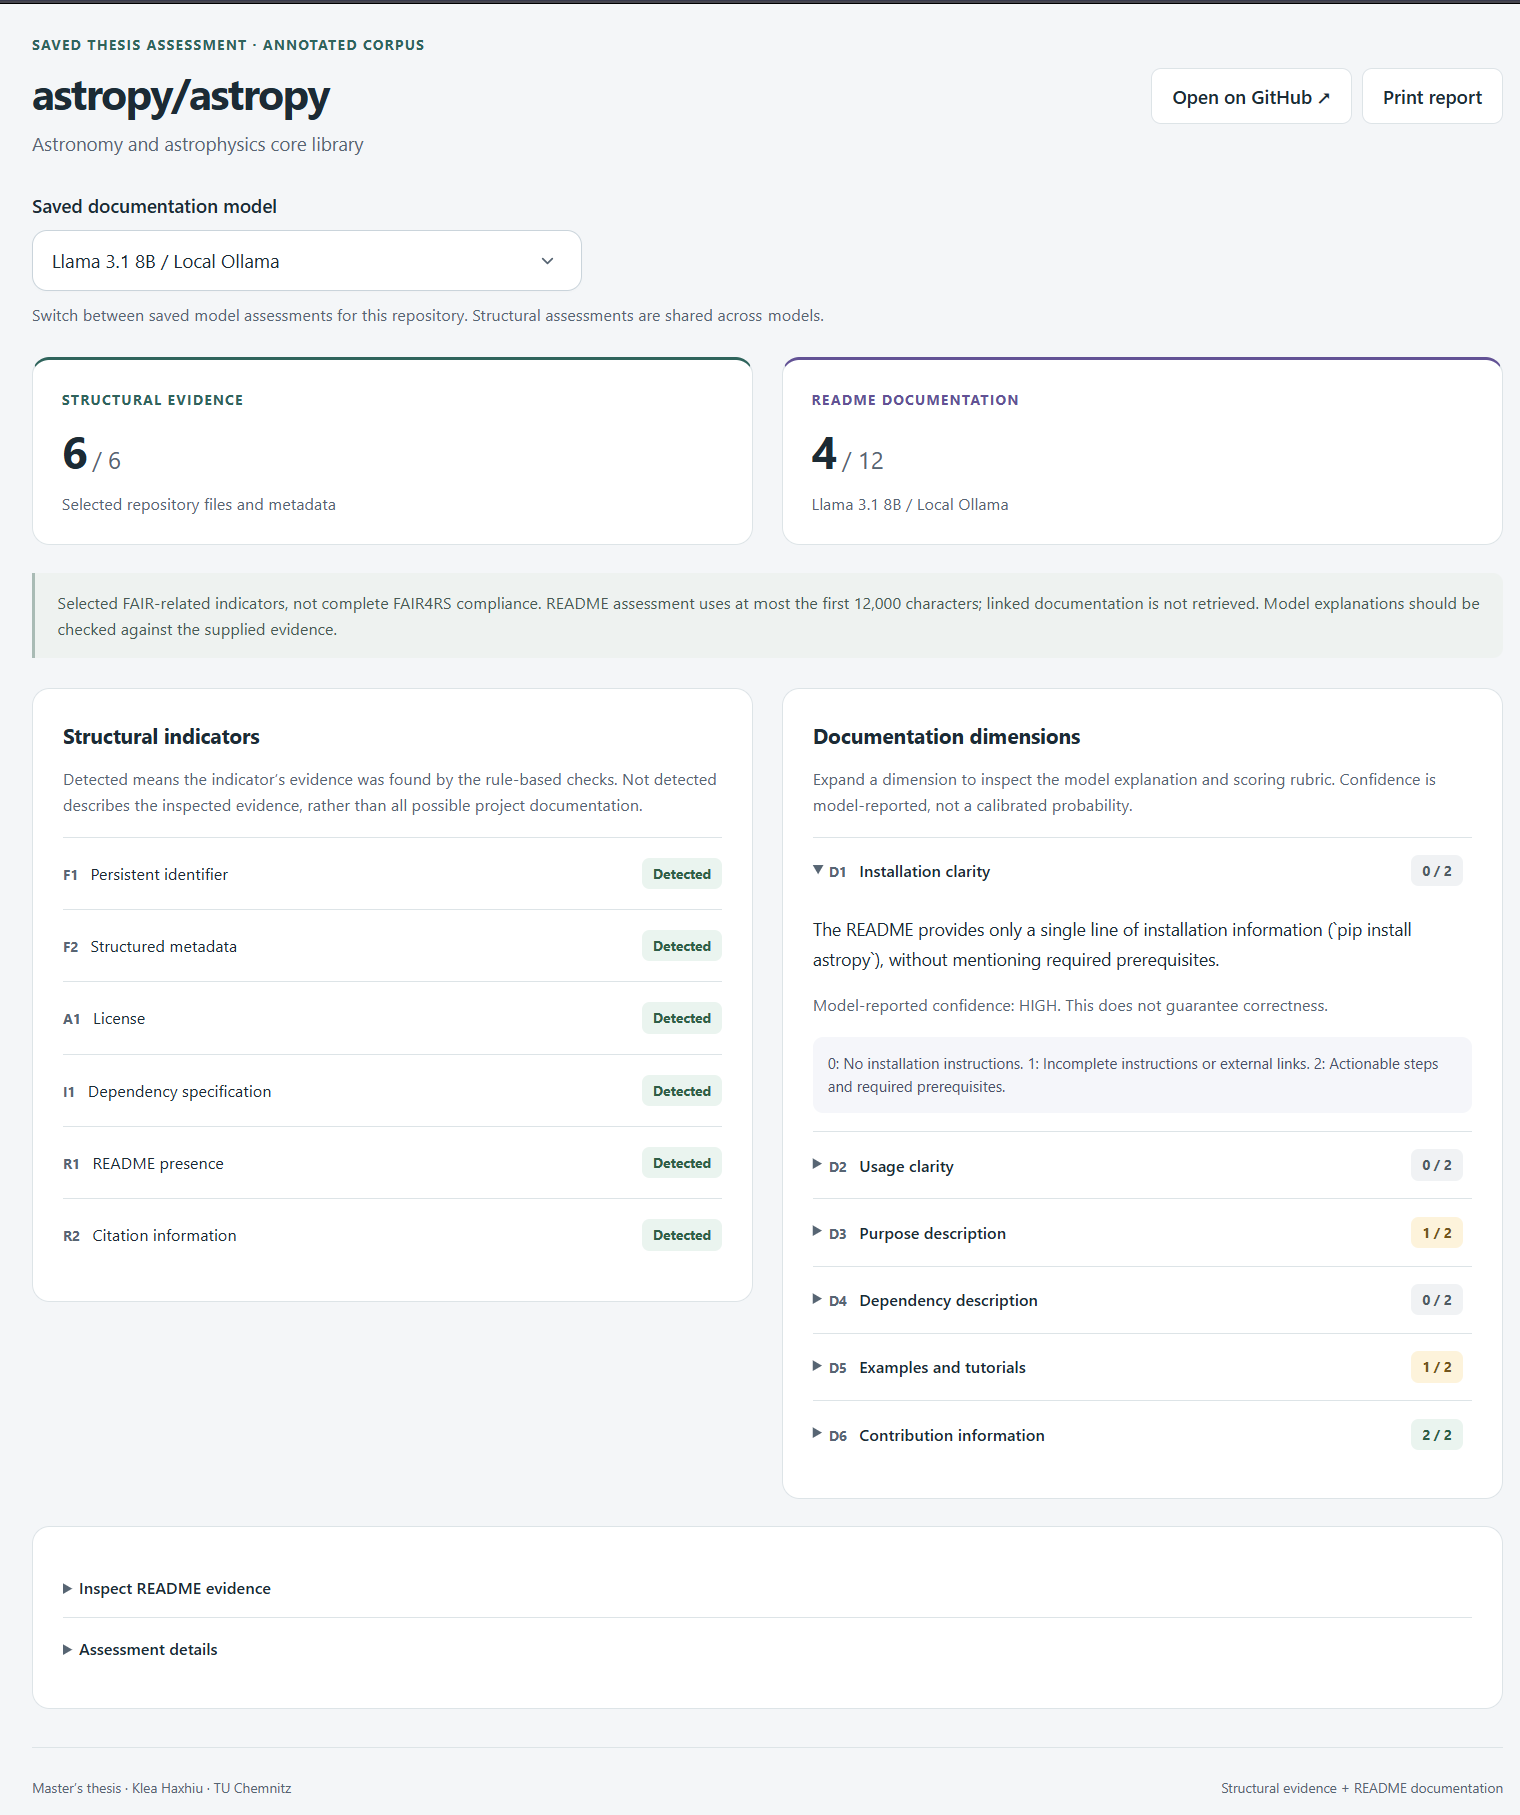
\includegraphics[
        width=\textwidth,
        height=0.78\textheight,
        keepaspectratio
    ]{figures/ui/web_repository_llama.png}
    \caption{Repository-level hybrid assessment for
    \texttt{astropy/astropy}. The interface presents deterministic
    structural indicators and the documentation assessment for the
    selected LLM configuration as separate components. Documentation
    dimensions can be expanded to inspect model-generated reasoning,
    reported confidence, and the scoring rubric, while the underlying
    README evidence and assessment metadata remain available for
    inspection.}
    \label{fig:web_repository}
\end{figure}

\FloatBarrier

\subsection{Live Repository Assessment}

In addition to inspecting saved thesis results, the prototype supports
assessment of a newly supplied public GitHub repository. The user
provides a repository identifier or GitHub URL and can request the
optional README documentation assessment. The backend retrieves the
current repository evidence and applies the same structural checks used
by the batch pipeline. 
When documentation assessment is enabled, the user can select the LLM
configuration used for the live assessment. Llama~3.1~8B is accessed
through the local Ollama service, whereas
\texttt{Qwen3.6-35B-A3B-MLX-8bit} is accessed through the university
KISTE service. The selected provider is handled by the backend, and
service availability or inference failures are reported explicitly
without discarding successfully computed structural results.

The resulting view preserves the same distinction between structural
and documentation-based assessment used for saved profiles. Each
documentation dimension can be expanded to inspect its score,
reasoning, confidence label, and rubric. Because these assessments
operate on current GitHub content, their results may differ from
previously collected repository snapshots. They are therefore treated
as interactive prototype results and remain separate from the fixed
experimental datasets used in Chapter~5.

As an implementation-level verification of the remote provider path, a
live assessment was successfully completed using the Qwen configuration
through the university KISTE service. This exercised the complete path
from retrieval of current GitHub repository evidence through remote LLM
inference and response validation to presentation of the resulting
hybrid profile. This verification concerns the operation of the web
prototype and is separate from the fixed experimental Qwen evaluation
reported in Chapter~5.

Figure~\ref{fig:web_live} shows a completed live assessment of
\texttt{pandas-dev/pandas}.

\begin{figure}[p]
    \centering
    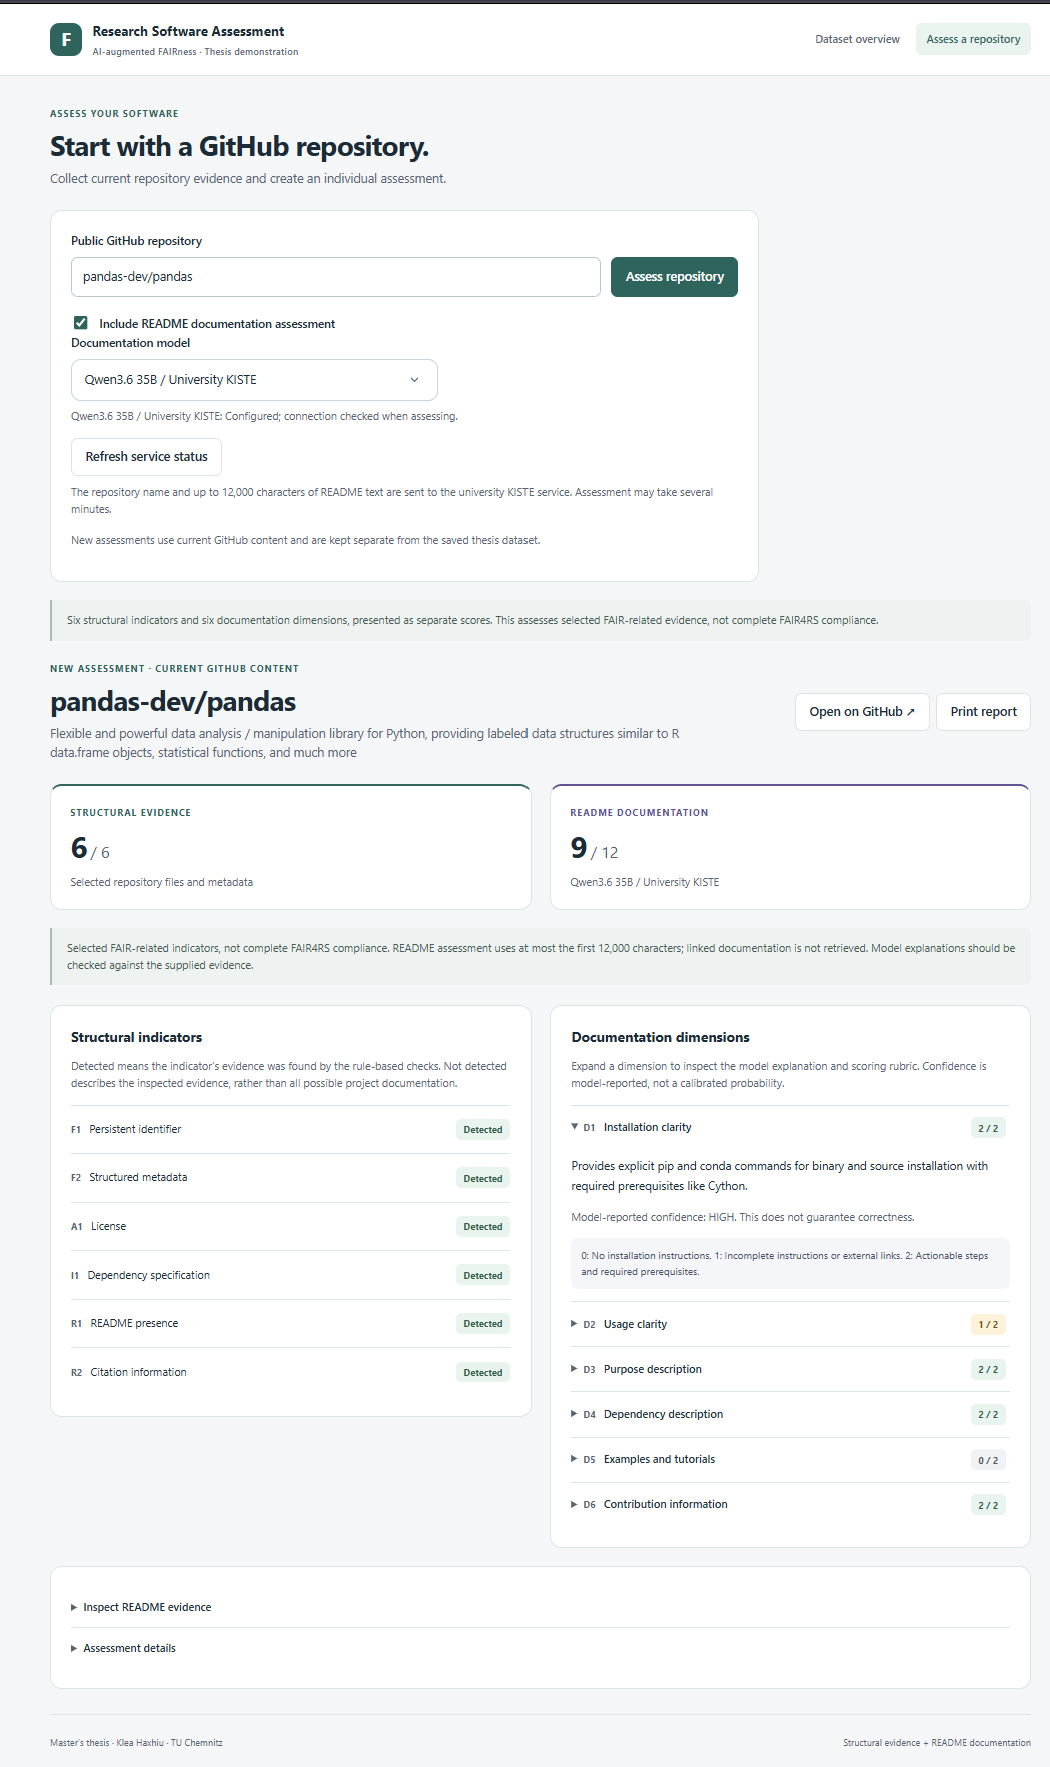
\includegraphics[
        width=\textwidth,
        height=0.78\textheight,
        keepaspectratio
    ]{figures/ui/web_live_qwen.png}
    \caption{Completed live assessment of \texttt{pandas-dev/pandas} using
the Qwen configuration through the university KISTE service. The
prototype retrieves current GitHub evidence, applies the deterministic
structural checks, and performs the optional README documentation
assessment. Structural and documentation scores remain separate, and
individual documentation dimensions expose the model-generated
reasoning, reported confidence, and scoring rubric.}
\label{fig:web_live}
\end{figure}

\FloatBarrier
\subsection{Implementation Limitations}

The web prototype inherits the evidence boundaries of the underlying
assessment pipeline. The qualitative component evaluates README
content only and does not retrieve documentation behind external
links. README input to the LLM is subject to the same 12{,}000-character
limit described in Chapter~3. Consequently, a live assessment should
be interpreted as an assessment of the evidence available to the
implemented framework rather than as a complete evaluation of all
documentation associated with a software project.

Live repository assessment additionally depends on access to GitHub,
while live documentation scoring depends on the selected LLM
provider. Llama assessment requires a configured local Ollama
instance, whereas Qwen assessment requires access to the university
KISTE service and a server-side authentication token. Authentication
credentials are not exposed to the frontend. Provider unavailability
or inference failure is reported to the user while preserving any
structural assessment that was successfully completed.
Model-reported confidence is displayed as contextual information and
is not presented as a calibrated probability of correctness.

\section{Implementation Summary}

This chapter has described the implementation of the proposed hybrid
FAIRness assessment framework. Its core assessment pipeline consists
of repository data collection, a rule-based assessment component, an
LLM-based documentation assessment component, and hybrid profile
generation. Repository data and assessment outputs are persisted using
local JSON and CSV files, allowing individual processing stages and
their underlying evidence to be inspected and re-run independently.

The documentation component supports two evaluated model
configurations: Llama~3.1~8B through local Ollama and
\texttt{Qwen3.6-35B-A3B-MLX-8bit} through the university KISTE
service. Model-specific documentation results are retained separately
and combined with the shared deterministic results without reducing
the two assessment components to a single score.

A web-based prototype was additionally implemented on top of the
assessment pipeline to make the resulting assessments directly
inspectable and to support assessment of newly supplied public GitHub
repositories. The interface exposes aggregate dataset summaries,
model-specific evaluation results, searchable access to saved
repository assessments, side-by-side comparison of the two LLM
configurations against human reference annotations, repository-level
hybrid profiles, underlying assessment evidence, model-generated
reasoning and confidence information, and live repository assessment
using either supported LLM provider.

Saved experimental results remain separated from live assessments so
that interactive use of the prototype does not modify the fixed
datasets evaluated in the following chapter. Throughout the interface,
structural and documentation-based results remain separate, preserving
the hybrid design of the proposed framework.

The following chapter evaluates the accuracy and reliability of the
assessment components against the manually annotated ground truth,
examines differences between the two evaluated LLM configurations, and
compares the proposed approach with existing FAIR assessment tools.

\chapter{Evaluation and Results}
\section{Experimental Setup}

This chapter presents the quantitative evaluation of the proposed 
hybrid FAIRness assessment framework. The results assess the 
reliability of the framework and compare its outputs against 
manually annotated ground truth and an existing baseline approach.

\subsection{Dataset}

The full dataset comprises 188 research software repositories
collected from GitHub across 10 research domains, as described in
Chapter~3. In addition, a manually annotated corpus of 30 repositories
was constructed to provide ground truth for quantitative evaluation.
The annotated corpus was selected to provide diversity across research
domains and programming languages, including repositories implemented
in Python, C++, Java, MATLAB, Fortran, Julia, Go, Rust, and Groovy.

Ten of the 30 annotated repositories were initially used during a
pilot phase to refine the annotation guidelines and assessment
procedure. These repositories were retained in the final annotated
corpus. To assess the effect of this original pilot overlap, the
remaining 20 repositories were additionally analysed as a
pilot-exclusion subset. For the LLM-based dimensions, these
repositories had not been used during pilot-phase refinement and
therefore provide a pilot-exclusion sensitivity check of LLM--human
agreement that is unaffected by the original pilot-phase refinement.
For the rule-based indicators, the same subset is used
only as an internal consistency check because some rule-based
annotations were corrected during final scorer validation.

\subsection{Evaluation Metrics}

The following metrics are used throughout this chapter:

\begin{description}
\item[Exact Match Accuracy] The proportion of repositories for 
which the automated score exactly matches the manual annotation. 
Reported as a percentage.

\item[Mean Absolute Error (MAE)] The average absolute difference 
between the automated assessment and the corresponding manual 
annotation, computed per dimension across all 30 ground truth 
repositories. Applied to the ordinal LLM-based dimensions (D1--D6).

\item[Cohen's Unweighted Kappa] Used for binary rule-based 
indicators (F1--R2), where any disagreement is treated equally 
regardless of magnitude.

\item[Cohen's Linearly Weighted Kappa] Used for ordinal AI-based 
dimensions (D1--D6), where partial agreement is given proportional 
credit. A disagreement of 1 point is penalised less than a 
disagreement of 2 points.
\end{description}

Kappa values are interpreted following the scale proposed by
Landis and Koch~\cite{landis1977kappa}: values below 0 indicate poor
agreement, 0.00--0.20 slight agreement, 0.21--0.40 fair agreement,
0.41--0.60 moderate agreement, 0.61--0.80 substantial agreement,
and 0.81--1.00 almost perfect agreement.

\subsection{Models and Tools}

The LLM-based component was evaluated using two model configurations.
The primary configuration uses \texttt{llama3.1:8b}, executed locally
through the Ollama HTTP API at temperature 0. The model was selected
because it can be executed locally without external API calls,
supporting reproducible assessment within the local experimental
environment. Structured JSON output is enforced through a schema that
constrains scores to the permitted values (0, 1, or 2).

To examine whether the observed LLM assessment behaviour was specific
to this model configuration, a second evaluation was conducted using
\texttt{Qwen3.6-35B-A3B-MLX-8bit}. The model was accessed through a
university-hosted OpenAI-compatible chat completion API and was applied
to the same 30-repository annotated corpus. The same D1--D6 dimensions,
scoring rubric, README-only evidence policy, 12,000-character input
limit, and temperature setting were retained. Backend-specific output
handling differed as described in Chapters~3 and~4.

The rule-based component operates deterministically on locally stored
repository snapshots. The howfairis tool is used as a software-oriented
baseline comparison. F-UJI, an automated FAIR assessment tool designed
primarily for research data objects, is additionally used in a pilot
experiment to investigate the applicability of an external,
data-oriented FAIR assessment baseline to research software
repositories.

\subsection{Experimental Environment}

The evaluation pipeline was implemented in Python. The primary Llama
configuration was executed locally on Windows using Ollama, with the
\texttt{llama3.1:8b} model (4.9~GB). The second model configuration,
\texttt{Qwen3.6-35B-A3B-MLX-8bit}, was accessed through the
university-hosted OpenAI-compatible API. All assessment scripts, input
data, parsed outputs, and derived evaluation results are stored in the
project repository to support reproducibility. Model-specific result
files are kept separate so that evaluations can be reproduced and
analysed independently.


\subsection{Evaluation Procedure}

The evaluation was conducted in the following order:

\begin{enumerate}

\item The thesis author manually annotated 30 ground truth
repositories against the finalised annotation guidelines (v1.4).

\item A second annotator independently annotated the same 30
repositories using the same guidelines.

\item Inter-annotator agreement was computed between the two
human annotators to validate the reliability of the ground truth.

\item The Llama-based scorer was applied to the 30 annotated
repositories and its outputs were compared against both human
annotators.

\item The Qwen-based scorer was independently applied to the same
30 repositories using the same documentation dimensions and scoring
rubric, and its outputs were likewise compared against both human
annotators.

\item The rule-based scorer was applied to all 188 repositories
to produce a complete set of structural FAIR indicator scores.

\item Hybrid FAIRness profiles were generated by combining the
shared rule-based results with the corresponding LLM results for
the 30 ground truth repositories. Separate profile sets were retained
for the two evaluated LLM configurations.

\item The howfairis baseline was executed on the 30 ground truth
repositories and compared against the proposed framework.

\item F-UJI was applied directly to a subset of five ground truth
repositories to investigate its applicability as an external
data-oriented FAIRness assessment baseline for research software.

\item As a sensitivity analysis, LLM--human agreement was recomputed
for both model configurations on the 20-repository pilot-exclusion
subset after excluding the 10 repositories used during pilot-phase
refinement. Rule-based performance was also recomputed on this subset
as an internal consistency check.

\end{enumerate}

\section{Ground Truth Validation}

\subsection{Annotation Process}

Manual annotations were created by the thesis author for all 30 
ground truth repositories following the finalised annotation 
guidelines (v1.4), as described in Chapter~3. Each repository was 
annotated by examining the repository root file structure and README 
content. Rule-based indicators (F1--R2) were assigned binary scores 
according to the annotation guidelines based on evidence obtained 
from the repository structure and README content. AI-based dimensions 
(D1--D6) were scored on a 0--2 ordinal scale based on the clarity 
and completeness of the README documentation.

To assess annotation reliability, a second annotator independently 
annotated the same 30 repositories using identical guidelines and 
pre-fetched repository data, without access to the primary 
annotations.

\subsection{Inter-Annotator Agreement}

Inter-annotator agreement between the two annotators was quantified 
using Cohen's unweighted Kappa for binary rule-based indicators and 
Cohen's linearly weighted Kappa for ordinal AI-based dimensions. 
Table~\ref{tab:iaa} presents the results.

\begin{table}[h]
\centering
\caption{Inter-annotator agreement for rule-based indicators and 
AI-based dimensions (n=30).}
\label{tab:iaa}
\begin{tabular}{llrrr}
\hline
\textbf{Indicator/Dimension} & \textbf{Type} & \textbf{$\kappa$} & 
\textbf{Exact} & \textbf{Interpretation} \\
\hline
F1 --- Persistent identifier & Binary & 0.710 & 90.0\% & Substantial \\
F2 --- Structured metadata   & Binary & 1.000 & 100.0\% & Almost perfect \\
A1 --- License               & Binary & undef. & 100.0\% & Single class \\
I1 --- Dependency file       & Binary & 0.634 & 93.3\% & Substantial \\
R1 --- README present        & Binary & undef. & 100.0\% & Single class \\
R2 --- Citation information  & Binary & 0.658 & 83.3\% & Substantial \\
\hline
\textbf{Rule macro-avg}      & & \textbf{0.750} & & \\
\hline
D1 --- Installation          & Ordinal & 0.539 & 70.0\% & Moderate \\
D2 --- Usage                 & Ordinal & 0.747 & 83.3\% & Substantial \\
D3 --- Purpose               & Ordinal & 0.789 & 96.7\% & Substantial \\
D4 --- Dependencies          & Ordinal & 0.743 & 80.0\% & Substantial \\
D5 --- Examples              & Ordinal & 0.585 & 70.0\% & Moderate \\
D6 --- Contribution          & Ordinal & 0.849 & 90.0\% & Almost perfect \\
\hline
\textbf{AI macro-avg}        & & \textbf{0.709} & & \\
\hline
\end{tabular}
\end{table}

Overall, the agreement results indicate that both the binary 
rule-based indicators and the ordinal documentation quality 
dimensions can be annotated consistently using the proposed 
guidelines.

The AI-based dimensions achieved a macro-average weighted Kappa of 
0.709, indicating substantial overall agreement between annotators. 
The strongest agreement was observed for D6 (contribution 
information, $\kappa$=0.849) and D3 (purpose description, 
$\kappa$=0.789). The weakest agreement was observed for D1 
(installation clarity, $\kappa$=0.539) and D5 (examples and 
tutorials, $\kappa$=0.585), suggesting greater ambiguity when 
assessing partially documented functionality or documentation 
provided through external links.

For the rule-based indicators, F2 achieved perfect agreement, while 
F1, I1, and R2 showed substantial agreement. Two indicators are 
mathematically undefined: R1 (README present), because all 30 
repositories have a README file, and A1 (license), because both 
annotators agreed on the presence of a license for all 30 
repositories following a correction described below. Both indicators 
demonstrate consistent annotation in practice, as reflected by their 
100\% exact agreement.

The rule-based macro-average of 0.750 excludes the two undefined 
values (A1 and R1).

I1 (dependency file present) initially showed disagreement on seven 
repositories, predominantly projects using non-Python language 
ecosystems (C++, Java, Go, Rust, Groovy, Julia), following the 
pattern that the primary annotator assigned a score of 0 while the 
second annotator assigned a score of 1. Investigation traced this to 
an incomplete file-detection schema used during ground-truth 
collection: the collector script for the 30 ground-truth repositories 
predated the expanded dependency-file list (including 
\texttt{go.mod}, \texttt{Cargo.toml}, \texttt{pom.xml}, 
\texttt{build.gradle}, and \texttt{Project.toml}) later adopted for 
the full 188-repository collection, and consequently could not 
detect language-specific dependency files for non-Python projects. 
Five of the seven affected repositories were confirmed via the 
corrected file inventory to genuinely contain a dependency 
specification file, and the corresponding primary annotations were 
corrected accordingly. Following this correction, I1 agreement 
improved from $\kappa$=0.286 (fair) to $\kappa$=0.634 (substantial).

A1 (license) was also corrected during validation: one repository 
(\texttt{rust-ml/linfa}) had been annotated as lacking a license, 
despite both the GitHub repository metadata and the README text 
explicitly identifying an Apache-2.0 license. This annotation was 
corrected, resulting in full agreement between annotators for A1.

Overall, these inter-annotator agreement results indicate a level of
annotation consistency that supports using the manual annotations as
the reference ground truth for the subsequent evaluation, while the
dimension-level differences are considered when interpreting the
LLM--human agreement results.

\section{Rule-Based Assessment Results}

The rule-based scorer was applied to all 188 repositories in the 
full dataset, producing binary scores for each of the six FAIR 
indicators (F1--R2). This section presents the distribution of 
rule-based assessment results across the full dataset and 
evaluates the rule-based component against the manually annotated 
ground truth repositories.

\subsection{Full Dataset Results}

Table~\ref{tab:rb_full} summarises the frequency of positive scores 
for each indicator across all 188 repositories.

\begin{table}[h]
\centering
\caption{Rule-based indicator frequencies across the full dataset 
(n=188).}
\label{tab:rb_full}
\begin{tabular}{llrr}
\hline
\textbf{Indicator} & \textbf{Description} & \textbf{Positive} & 
\textbf{Percentage} \\
\hline
F1 & Persistent identifier & 95 & 51\% \\
F2 & Software metadata     & 58 & 31\% \\
A1 & License               & 182 & 97\% \\
I1 & Dependency file       & 123 & 65\% \\
R1 & README present        & 188 & 100\% \\
R2 & Citation information  & 79 & 42\% \\
\hline
\end{tabular}
\end{table}

All 188 repositories contain a README file (R1=100\%), and 97\% 
have a license file (A1=97\%). In contrast, dedicated software 
metadata files such as \texttt{CITATION.cff} or 
\texttt{codemeta.json} are present in only 31\% of repositories 
(F2), and persistent identifiers such as DOIs or Zenodo badges 
are present in only 51\% (F1). Citation information is available 
in 42\% of repositories (R2), suggesting that fewer than half of 
the evaluated repositories provide explicit guidance on how to 
cite the software. Overall, the results indicate that basic 
repository documentation practices, such as providing README and 
license files, are widespread, whereas richer FAIR-related metadata 
and citation support remain considerably less common.

The mean rule-based score across the full dataset was 3.86 out of 
a maximum possible score of 6. The score distribution is shown in 
Table~\ref{tab:rb_dist}.

\begin{table}[h]
\centering
\caption{Distribution of rule-based total scores across the full 
dataset (n=188).}
\label{tab:rb_dist}
\begin{tabular}{rrr}
\hline
\textbf{Score} & \textbf{Count} & \textbf{Percentage} \\
\hline
6/6 & 15  & 8\%  \\
5/6 & 43  & 23\% \\
4/6 & 61  & 32\% \\
3/6 & 42  & 22\% \\
2/6 & 23  & 12\% \\
1/6 & 4   & 2\%  \\
\hline
\end{tabular}
\end{table}

The score distribution spans the full range from 1 to 6, indicating
substantial variability in the structural FAIR-related indicators
assessed across the dataset. Only 15 repositories (8\%) satisfy all
six rule-based indicators, while 27 repositories (14\%) satisfy two
or fewer, indicating gaps in the structural evidence captured by the
assessment.


\subsection{Validation Against Ground Truth}

The rule-based scorer was validated against the final manual
annotations for the 30 ground truth repositories. During validation,
differences between automated predictions and manual annotations
were inspected individually and resolved according to the finalised
annotation guidelines (v1.4).

This process identified both implementation-level detection gaps and
manual annotation inconsistencies, particularly affecting the citation
(R2), persistent identifier (F1), and license (A1) indicators. The
rule-based detection logic was refined to recognise additional valid
citation and persistent identifier patterns, including
\texttt{CITATION.cff} files, generic DOI representations, and explicit
citation wording. Manual annotations that were inconsistent with the
final rubric were corrected and documented in the corresponding
repository annotation files.

After these refinements, the final rule-based scorer achieved exact
agreement with the final ground truth annotations across all 30
repositories. Precision, recall, and F1-score were 1.000 for each of
the six binary indicators (F1--R2), as shown in
Table~\ref{tab:rule_prf}.

\begin{table}[h]
\centering
\caption{Rule-based validation against manual ground truth (n=30).}
\label{tab:rule_prf}
\begin{tabular}{lrrr}
\hline
\textbf{Indicator} & \textbf{Precision} & \textbf{Recall} &
\textbf{F1-score} \\
\hline
F1 --- Persistent identifier & 1.000 & 1.000 & 1.000 \\
F2 --- Software metadata     & 1.000 & 1.000 & 1.000 \\
A1 --- License               & 1.000 & 1.000 & 1.000 \\
I1 --- Dependency file       & 1.000 & 1.000 & 1.000 \\
R1 --- README present        & 1.000 & 1.000 & 1.000 \\
R2 --- Citation information  & 1.000 & 1.000 & 1.000 \\
\hline
\end{tabular}
\end{table}

The final results demonstrate that the rule-based implementation
faithfully reproduces the operational definitions encoded in the
finalised manual annotation rubric for the evaluated ground-truth
corpus. Because scorer refinements and corrections to some rule-based
annotations were made during final validation, the resulting perfect
agreement should not be interpreted as an unbiased estimate of
performance on unseen repositories. The additional pilot-exclusion
analysis in Section~\ref{sec:pilot_exclusion_sensitivity} therefore
serves as an internal consistency check for the rule-based component 
rather than as independent validation.
\section{LLM-Based Assessment Results}
Two model configurations, \texttt{llama3.1:8b} and
\texttt{Qwen3.6-35B-A3B-MLX-8bit}, were evaluated on the same
30-repository ground-truth corpus. Both configurations assessed
the same six documentation dimensions (D1--D6) using the same scoring
rubric and README-only evidence policy.

The following analysis compares each model independently against both
human annotators. The purpose of the second model evaluation is not to
establish a general ranking between models, but to examine whether the
observed reliability and failure patterns are specific to the primary
Llama configuration or recur under a different LLM configuration.

\subsection{Agreement with the Primary Annotator}

Table~\ref{tab:llm_a1} presents the agreement of both LLM
configurations with the primary annotator. Weighted Cohen's Kappa,
exact agreement, and mean absolute error are reported independently
for each documentation dimension.

\begin{table}[htbp]
\centering
\caption{Agreement of the two LLM configurations with the primary
annotator (n=30).}
\label{tab:llm_a1}
\small
\begin{tabular}{lrrrrrr}
\hline
& \multicolumn{3}{c}{\textbf{Llama 3.1 8B}}
& \multicolumn{3}{c}{\textbf{Qwen3.6-35B-A3B-MLX-8bit}} \\
\cline{2-4}\cline{5-7}
\textbf{Dimension}
& \textbf{$\kappa$} & \textbf{Exact} & \textbf{MAE}
& \textbf{$\kappa$} & \textbf{Exact} & \textbf{MAE} \\
\hline
D1 --- Installation
& 0.605 & 70.0\% & 0.333
& 0.799 & 86.7\% & 0.133 \\
D2 --- Usage
& 0.274 & 46.7\% & 0.567
& 0.516 & 70.0\% & 0.300 \\
D3 --- Purpose
& $-$0.071 & 86.7\% & 0.133
& 0.789 & 96.7\% & 0.033 \\
D4 --- Dependencies
& 0.480 & 60.0\% & 0.433
& 0.487 & 56.7\% & 0.433 \\
D5 --- Examples
& 0.192 & 36.7\% & 0.700
& 0.320 & 43.3\% & 0.567 \\
D6 --- Contribution
& 0.494 & 63.3\% & 0.400
& 0.759 & 83.3\% & 0.167 \\
\hline
\textbf{Macro-avg. $\kappa$}
& \textbf{0.329} & & 
& \textbf{0.612} & & \\
\hline
\end{tabular}
\end{table}

The results differ substantially between the two model
configurations. Llama achieved a macro-average weighted Kappa of
0.329 against the primary annotator, whereas Qwen achieved 0.612.
The latter therefore showed substantially stronger agreement with
the manual annotations in this experiment.

For Qwen, the strongest agreement was observed for installation
(D1, $\kappa$=0.799), purpose (D3, $\kappa$=0.789), and contribution
information (D6, $\kappa$=0.759). Usage documentation achieved
moderate agreement (D2, $\kappa$=0.516), while dependencies
(D4, $\kappa$=0.487) and examples (D5, $\kappa$=0.320) remained
more difficult.

The contrast for D3 is particularly pronounced. Llama achieved a
weighted Kappa of $-$0.071 despite 86.7\% exact agreement, whereas
Qwen achieved $\kappa$=0.789 with 96.7\% exact agreement. The
negative Llama value occurs in a dimension with strongly imbalanced
human scores and should therefore be interpreted together with its
high exact agreement. At the same time, the substantially stronger
Qwen result shows that the weak Kappa observed for Llama is not a
consistent property of LLM-based purpose assessment across the two
evaluated configurations.

Overall, these results indicate that agreement with human assessment
is both model-dependent and dimension-dependent. The second model
substantially improves agreement for several dimensions, but the
remaining variation across D1--D6 shows that stronger overall
performance does not remove dimension-specific assessment
difficulties.

\subsection{Agreement with the Second Annotator}

To examine whether the model--human agreement patterns depend on the
choice of human reference, both model configurations were also
compared with the second annotator. Table~\ref{tab:llm_a2} presents
the results.

\begin{table}[htbp]
\centering
\caption{Agreement of the two LLM configurations with the second
annotator (n=30).}
\label{tab:llm_a2}
\small
\begin{tabular}{lrrrr}
\hline
\textbf{Dimension}
& \textbf{Llama $\kappa$}
& \textbf{Llama Exact}
& \textbf{Qwen $\kappa$}
& \textbf{Qwen Exact} \\
\hline
D1 --- Installation & 0.480 & 70.0\% & 0.429 & 63.3\% \\
D2 --- Usage        & 0.276 & 50.0\% & 0.488 & 66.7\% \\
D3 --- Purpose      & $-$0.056 & 86.7\% & 1.000 & 100.0\% \\
D4 --- Dependencies & 0.338 & 53.3\% & 0.481 & 60.0\% \\
D5 --- Examples     & 0.156 & 30.0\% & 0.133 & 13.3\% \\
D6 --- Contribution & 0.454 & 60.0\% & 0.809 & 86.7\% \\
\hline
\textbf{Macro-avg. $\kappa$}
& \textbf{0.275} & & \textbf{0.557} & \\
\hline
\end{tabular}
\end{table}

The comparison with the second annotator shows the same broad
model-level pattern. Llama achieved a macro-average weighted Kappa
of 0.275, whereas Qwen achieved 0.557. Qwen again showed particularly
strong agreement for purpose (D3, $\kappa$=1.000) and contribution
information (D6, $\kappa$=0.809).

However, the second-annotator comparison also highlights the
sensitivity of dimension-level results to the human reference.
Most notably, Qwen agreement for examples (D5) decreased to
$\kappa$=0.133, compared with 0.320 against the primary annotator.
This is consistent with the lower human--human agreement previously
observed for D5 and reinforces that some documentation dimensions
contain greater interpretive variation than others.

Taken together, the two annotator comparisons show that Qwen achieved
higher macro-average agreement than Llama against both human
references, while the magnitude of agreement remained dependent on
both the assessed dimension and the human reference annotation.

\subsection{Pilot-Exclusion Sensitivity Analysis}
\label{sec:pilot_exclusion_sensitivity}

Because 10 of the 30 annotated repositories had been used during
pilot-phase refinement, final-system results were additionally
examined after excluding these repositories. The resulting
20-repository subset provides a pilot-exclusion sensitivity check for
the LLM-based dimensions, which were not modified during this
validation process. For the rule-based component, however, the
analysis should be interpreted more cautiously: several manual
rule-based annotations within this subset were corrected during
final scorer validation after inconsistencies in the annotation
evidence and detection schema were identified. The rule-based
20-repository result is therefore reported as an internal consistency
check rather than as independent validation.

For the rule-based component, precision, recall, and F1-score were
1.000 for all six indicators after exclusion of the 10 original
pilot repositories. Because some rule-based annotations in this
subset were corrected during final validation, this result confirms
consistency between the final scorer and finalised annotation rubric
but should not be interpreted as an unbiased estimate of performance
on unseen repositories.

For the LLM-based component, Table~\ref{tab:llm_pilot_exclusion}
compares agreement with the primary annotator on the full annotated
corpus and the 20-repository pilot-exclusion subset for both model
configurations.

\begin{table}[htbp]
\centering
\caption{LLM agreement with the primary annotator on the full
annotated corpus and the 20-repository pilot-exclusion subset.}
\label{tab:llm_pilot_exclusion}
\small
\begin{tabular}{lrrrr}
\hline
\textbf{Dimension}
& \textbf{Llama (n=30)}
& \textbf{Llama (n=20)}
& \textbf{Qwen (n=30)}
& \textbf{Qwen (n=20)} \\
\hline
D1 --- Installation
& 0.605 & 0.659 & 0.799 & 0.787 \\
D2 --- Usage
& 0.274 & 0.474 & 0.516 & 0.531 \\
D3 --- Purpose
& $-$0.071 & $-$0.071 & 0.789 & 0.783 \\
D4 --- Dependencies
& 0.480 & 0.337 & 0.487 & 0.405 \\
D5 --- Examples
& 0.192 & 0.286 & 0.320 & 0.367 \\
D6 --- Contribution
& 0.494 & 0.556 & 0.759 & 0.815 \\
\hline
\textbf{Macro-avg.}
& \textbf{0.329}
& \textbf{0.373}
& \textbf{0.612}
& \textbf{0.615} \\
\hline
\end{tabular}
\end{table}

For Llama, excluding the 10 pilot repositories did not reduce
agreement with the primary annotator. The macro-average weighted
Kappa increased from 0.329 on the complete 30-repository corpus to
0.373 on the 20-repository pilot-exclusion subset. Agreement increased
for D1, D2, D5, and D6, remained unchanged for D3, and decreased for
D4.

The Qwen results were even more stable across the two populations.
Its macro-average weighted Kappa was 0.612 on the complete annotated
corpus and 0.615 after exclusion of the 10 pilot repositories.
Dimension-level agreement also remained broadly similar: D1 and D3
decreased only slightly, D2 and D5 increased slightly, D6 increased
from 0.759 to 0.815, and D4 decreased from 0.487 to 0.405.

Since neither LLM scorer nor the D1--D6 annotations in the
20-repository subset were modified as part of the rule-based
validation corrections, these results provide a sensitivity check
for the effect of the original pilot overlap on LLM--human agreement.
For both model configurations, exclusion of the pilot repositories
did not weaken the overall agreement result. In particular, the
near-identical Qwen macro-average values on the full corpus and the
pilot-exclusion subset indicate that its observed agreement was not
primarily driven by the 10 repositories involved in the original
pilot phase.

The rule-based results likewise remain internally consistent after
pilot exclusion. However, their perfect performance should not be
interpreted as independent generalisation evidence because some
rule-based annotations within this subset were corrected during final
scorer validation.

\subsection{Systematic Scoring Patterns}
\label{sec:llm_systematic_patterns}

Analysis of the direction of disagreements reveals that both model
configurations tended to assign lower scores than the primary human
annotator, although the dimensions in which this behaviour was most
pronounced differed between models. Table~\ref{tab:llm_dir}
summarises the direction of disagreements for both configurations.

\begin{table}[htbp]
\centering
\caption{Direction of LLM scoring disagreements relative to the
primary annotator (n=30). Lower indicates model score $<$ human score;
higher indicates model score $>$ human score.}
\label{tab:llm_dir}
\small
\begin{tabular}{lrrrr}
\hline
\textbf{Dimension}
& \textbf{Llama lower}
& \textbf{Llama higher}
& \textbf{Qwen lower}
& \textbf{Qwen higher} \\
\hline
D1 --- Installation  & 8  & 1 & 2  & 2 \\
D2 --- Usage         & 14 & 2 & 6  & 3 \\
D3 --- Purpose       & 2  & 2 & 1  & 0 \\
D4 --- Dependencies  & 8  & 4 & 13 & 0 \\
D5 --- Examples      & 17 & 2 & 17 & 0 \\
D6 --- Contribution  & 9  & 2 & 4  & 1 \\
\hline
\end{tabular}
\end{table}

For Llama, the most pronounced underscoring occurred for D5
(examples and tutorials), with 17 lower scores compared with two
higher scores, and D2 (usage clarity), with 14 lower scores compared
with two higher scores. These dimensions are particularly sensitive
to the README-only evidence policy adopted in this study. Relevant
usage guidance, tutorials, and example material may be provided
through external documentation links that are not followed during
the automated assessment.

Qwen reduced the frequency of disagreement for several dimensions,
particularly D1, D2, D3, and D6. However, systematic underscoring
remained pronounced for D4 and D5. For dependency documentation
(D4), Qwen assigned a lower score than the primary annotator in
13 of 30 repositories and never assigned a higher score. For examples
and tutorials (D5), it assigned a lower score in 17 repositories and
again never assigned a higher score. Against the second annotator,
the D5 tendency was even more pronounced, with Qwen assigning a lower
score in 26 of 30 repositories.

The persistence of the D5 pattern across both model configurations
indicates that examples and tutorial evidence remain particularly
difficult under the implemented README-only assessment design.
The Qwen results additionally identify dependency documentation
(D4) as a recurring source of conservative scoring for the second
model configuration. These patterns show that stronger aggregate
agreement does not eliminate systematic dimension-specific
disagreements.

Purpose description (D3) illustrates a different form of
model-dependent behaviour. Llama produced a negative weighted Kappa
($\kappa=-0.071$) despite 86.7\% exact agreement with the primary
annotator. Human scores for this dimension were strongly concentrated
at score 2, with 28 of 30 repositories receiving that score, making
Kappa particularly sensitive to the small number of disagreements.
Qwen, however, agreed with the primary annotator on 29 of 30
repositories and achieved $\kappa=0.789$, while reaching exact
agreement with the second annotator on all 30 repositories
($\kappa=1.000$). The contrast demonstrates that the weak Llama D3
Kappa was not reproduced by the second model configuration.

Overall, the disagreement patterns reinforce the distinction between
model-level and dimension-level reliability. Qwen achieved stronger
aggregate agreement than Llama in this experiment, but dependencies
and examples remained substantially more difficult than dimensions
such as installation, purpose, and contribution information.

\subsection{Comparison with Inter-Annotator Agreement}

Table~\ref{tab:agreement_summary} places the model--human agreement
results alongside the agreement observed between the two human
annotators.

\begin{table}[htbp]
\centering
\caption{Agreement summary for human--human and model--human
comparisons (macro-average weighted $\kappa$, D1--D6).}
\label{tab:agreement_summary}
\begin{tabular}{lr}
\hline
\textbf{Comparison} & \textbf{Macro-avg. $\kappa$} \\
\hline
Human A1 vs Human A2 & 0.709 \\
Llama vs Human A1    & 0.329 \\
Llama vs Human A2    & 0.275 \\
Qwen vs Human A1     & 0.612 \\
Qwen vs Human A2     & 0.557 \\
\hline
\end{tabular}
\end{table}

The two model configurations show substantially different levels of
agreement with the human annotations. Llama achieved macro-average
weighted Kappa values of 0.329 and 0.275 against the primary and
second annotators, respectively. Qwen achieved higher values of
0.612 and 0.557 against the same two references.

Human--human agreement was 0.709. This value provides useful context
for interpreting the model results, but it should not be treated as
a formal upper bound on achievable model performance. The Qwen
results nevertheless lie considerably closer to the observed
human--human agreement than the Llama results.

The same broad ordering is observed against both human references,
while the dimension-level results vary substantially. This indicates
that reliability cannot be characterised solely as a property of
``LLM-based assessment'' in general. Within the present experiment,
agreement depends materially on the model configuration, the
documentation dimension being assessed, and, to a lesser extent,
the human annotation used as the reference.

\subsection{Model-Reported Confidence Analysis}

Both LLM configurations produced a self-reported confidence label
(HIGH, MEDIUM, or LOW) for each documentation-quality score. To
examine whether these labels provide information about assessment
reliability, the 180 dimension-level predictions produced by each
model (30 repositories $\times$ 6 dimensions) were analysed relative
to the primary human annotations.

For Llama, predictions were distributed across all three confidence
levels. Table~\ref{tab:confidence_calibration} reports exact
agreement, mean absolute error (MAE), and linearly weighted Cohen's
Kappa within each confidence group.

\begin{table}[htbp]
\centering
\caption{Llama agreement with the primary human annotations grouped
by model-reported confidence across all documentation dimensions.}
\label{tab:confidence_calibration}
\begin{tabular}{lrrrr}
\hline
\textbf{Confidence} & \textbf{n} & \textbf{Exact} &
\textbf{MAE} & \textbf{$\kappa$} \\
\hline
HIGH   & 113 & 56.6\% & 0.460 & 0.520 \\
MEDIUM & 60  & 71.7\% & 0.283 & 0.478 \\
LOW    & 7   & 28.6\% & 1.143 & $-$0.120 \\
\hline
\end{tabular}
\end{table}

For Llama, the reported confidence levels were not monotonically
associated with prediction accuracy. MEDIUM-confidence predictions
achieved the highest exact agreement (71.7\%) and lowest MAE (0.283),
whereas HIGH-confidence predictions achieved lower exact agreement
(56.6\%) and a higher MAE (0.460). LOW-confidence predictions
performed worst, with 28.6\% exact agreement and an MAE of 1.143,
although this group contained only seven predictions and should
therefore be interpreted cautiously.

The dimension-level results also show that HIGH confidence did not
consistently indicate stronger agreement. For example, Llama's
HIGH-confidence predictions for D3 achieved 94.4\% exact agreement,
whereas HIGH-confidence predictions for D5 achieved only 29.4\%.
MEDIUM-confidence predictions also exceeded HIGH-confidence
predictions in exact agreement for D1, D2, D4, and D5.

The Qwen configuration exhibited a different confidence pattern.
All 180 dimension-level predictions were assigned HIGH confidence;
no MEDIUM- or LOW-confidence predictions were produced. Consequently,
confidence calibration across confidence levels could not be
evaluated for this model. Across the pooled HIGH-confidence
predictions, exact agreement with the primary annotator was 72.8\%,
MAE was 0.272, and weighted Kappa was 0.662. These pooled values
describe overall performance among predictions that all received the
same confidence label and should not be interpreted as evidence of
confidence calibration.

The uniform Qwen confidence assignment was not reflective of the
substantial variation in observed dimension-level agreement. Exact
agreement ranged from 43.3\% for examples and tutorials (D5) to
96.7\% for purpose description (D3), despite both dimensions
receiving HIGH confidence for every assessed repository. Thus,
Qwen's self-reported confidence did not provide a discriminative
reliability signal in this experiment.

Taken together, the two configurations demonstrate different
limitations of self-reported confidence. Llama produced multiple
confidence levels, but these were not monotonically related to
agreement with human assessment. Qwen produced no confidence
variation at all, preventing discrimination between more and less
reliable predictions. Model-reported confidence is therefore retained
as contextual information in the hybrid FAIRness profile rather than
treated as a calibrated quantitative estimate of assessment
correctness.


\subsection{README Length and Verbosity Bias}

To investigate whether either LLM configuration systematically
assigned relatively higher or lower scores to repositories with
longer README files, README length was compared with the difference
between each model's total documentation score and the corresponding
primary human total. README length was measured as the number of words
in the effective README text supplied to the model after applying the
12,000-character preprocessing limit.

For Llama, Spearman's rank correlation showed a weak negative and
non-significant relationship between effective README length and
model--human score difference ($\rho=-0.169$, $p=0.371$, $n=30$).
For Qwen, the corresponding relationship was similarly weak and
non-significant ($\rho=-0.143$, $p=0.451$, $n=30$). Thus, neither
model showed evidence at the repository level that longer README
files systematically produced relatively higher documentation scores
in the evaluated sample.

For Llama, dimension-level correlations were also non-significant,
with coefficients ranging from $\rho=-0.180$ for dependency
documentation (D4) to $\rho=0.060$ for installation documentation
(D1). In particular, D2 and D5, which showed pronounced Llama
underscoring, had weak negative correlations of $\rho=-0.110$ and
$\rho=-0.135$, respectively.

For Qwen, most dimension-level relationships were likewise weak and
non-significant. D4 was the exception, showing a negative association
between effective README length and model--human score difference
($\rho=-0.392$, $p=0.032$). This direction is consistent with the
systematic Qwen underscoring observed for D4. However, this result is
treated as exploratory because it arises from a dimension-level
analysis across six dimensions with only 30 repositories and no
multiple-comparison correction. It therefore does not provide a
basis for concluding that README length causes the D4 disagreement.

Only one of the 30 README files exceeded the 12,000-character input
limit. Inspection of the excluded portion showed that it consisted
of reStructuredText definitions for images, badges, logos, and
associated links rather than substantive documentation corresponding
to D1--D6. No relevant assessment evidence was identified as lost
through truncation in this particular case. Nevertheless, this
observation concerns only one repository, and the fixed sequential
cutoff may remove relevant sections in other long READMEs.

Overall, the repository-level analyses provide no evidence of a
systematic README verbosity bias for either evaluated model
configuration. This result is limited to the present 30-repository
sample and should not be interpreted as evidence that README length
or truncation effects cannot occur in a broader repository
population.

\section{Hybrid FAIRness Profile Analysis}

The hybrid FAIRness profile presents the rule-based indicators
(F1--R2) and LLM-based documentation quality scores (D1--D6)
together in a single structured record per repository while
preserving them as separate assessment dimensions. No overall
scalar FAIRness score is computed across the two components.
This section analyses the profiles for the 30 ground truth
repositories and examines the relationship between the two
assessment dimensions.
\subsection{Score Distributions}

Table~\ref{tab:hybrid_summary} presents descriptive scores for the
rule-based component and the primary Llama-based documentation
component across the 30 ground truth repositories.

\begin{table}[h]
\centering
\caption{Mean rule-based and primary Llama-based documentation scores
across the 30 ground truth repositories.}
\label{tab:hybrid_summary}
\begin{tabular}{lrr}
\hline
\textbf{Component} & \textbf{Mean Score} & \textbf{Maximum} \\
\hline
Rule-based total & 4.30 & 6 \\
Llama documentation total & 6.70 & 12 \\
\hline
\end{tabular}
\end{table}

The mean rule-based score across the 30 ground truth repositories was
4.30 out of 6, slightly higher than the mean of 3.86 across the full
188-repository dataset. The mean documentation score produced by the
primary Llama configuration was 6.70 out of 12.

These totals are reported only as descriptive summaries within their
respective assessment components. They are not combined or interpreted
as a single overall FAIRness score. Although a corresponding hybrid profile set was also generated using the
Qwen results, the purpose of the second model evaluation is to assess the
robustness of the LLM-based assessment findings rather than to replace the
primary Llama-based profile.

\subsection{Relationship Between Rule-Based and LLM Scores}

To examine whether repositories that score highly on structural FAIR
indicators also score highly on documentation quality, Spearman's rank
correlation was computed between the rule-based total and the documentation
total produced by each LLM configuration across the 30 ground truth
repositories.

For Llama, the correlation was weak and not statistically significant
($\rho=0.175$, $p=0.356$). Applying the same analysis to the Qwen-based
hybrid profiles also yielded a weak, non-significant correlation
($\rho=0.134$, $p=0.480$). No clear monotonic association was therefore
detected between the structural and documentation components for either
model in the evaluated sample.

These results are consistent with the design decision to preserve structural
FAIR-related indicators and qualitative documentation assessment as
separate dimensions of the hybrid profile. A repository may achieve a
high rule-based score through the presence of formal metadata and
repository artefacts while providing limited inline documentation.
Conversely, a repository may provide clear and useful README
documentation while lacking persistent identifiers, structured
metadata, or explicit citation information.

The Qwen analysis uses the same structural scores and the same
30 repositories as the Llama analysis, changing only the model-specific
documentation totals. The similar findings indicate that the absence
of a clear association in this sample is not specific to the primary
Llama configuration. However, non-significant correlations in this
small sample do not establish independence between the two assessment
components.

\subsection{Complementary Assessment Dimensions}

The evaluated repositories exhibited complementary assessment 
patterns. Repositories with high rule-based scores but comparatively low
documentation scores may possess strong structural FAIR-related
evidence while providing limited inline documentation. Conversely, 
other repositories achieve higher documentation scores despite 
lacking formal metadata such as \texttt{CITATION.cff} files or 
persistent identifiers.

By presenting both dimensions in parallel, the hybrid profile 
allows users to identify specific FAIRness gaps and prioritise 
improvements accordingly, rather than receiving a single aggregated 
score that obscures the nature of any deficiencies.

\subsection{Profile Interpretation}

The hybrid FAIRness profile provides information from both structural
and documentation-based assessment that is not represented by either
component alone. A repository with high scores in both components
shows strong coverage of the assessed structural FAIR-related
indicators together with strong README documentation according to the
qualitative assessment rubric.

Conversely, a repository with a high rule-based score but a low
documentation score may satisfy many of the assessed structural
indicators while providing limited documentation for practical reuse.
Similarly, a repository with lower rule-based scores but higher
documentation scores may provide strong README documentation while
lacking structural evidence such as persistent identifiers or
machine-readable citation metadata.

The evaluation with two LLM configurations additionally shows that
the documentation component is sensitive to the model used to produce
it. The hybrid representation itself is model-independent in the
sense that the structural and documentation dimensions remain
separate, but the reliability analysis demonstrates that individual
D1--D6 scores should be interpreted with awareness of the underlying
model configuration and its dimension-specific agreement behaviour.

\section{Baseline Comparison}

This section compares the proposed hybrid assessment framework 
with two existing FAIR assessment approaches. The software-oriented 
howfairis tool is evaluated across all 30 ground truth repositories 
and provides a direct comparison of assessment scope. F-UJI is 
examined separately through a five-repository pilot to determine 
whether a data-oriented FAIR assessment tool can provide a 
meaningful quantitative baseline when applied directly to research 
software repositories hosted on GitHub.

\subsection{F-UJI Baseline Applicability}
\label{sec:fuji_baseline}

Before using F-UJI as a quantitative baseline, its applicability 
to research software repositories was investigated. F-UJI is 
designed primarily for assessing the FAIRness of research data 
objects. The pilot therefore examined whether it could meaningfully 
differentiate research software repositories when provided with 
plain GitHub repository URLs.

Five ground truth repositories with different rule-based and 
documentation quality profiles were submitted directly to F-UJI 
(version 3.5.1, metrics v0.8): \texttt{astropy/astropy} and 
\texttt{sunpy/sunpy} with rule-based scores of 6/6, 
\texttt{gonum/gonum} with a rule-based score of 2/6 and an LLM 
documentation score of 4/12, \texttt{yt-project/yt} with scores 
of 3/6 and 10/12, respectively, and \texttt{scipy/scipy} with 
scores of 5/6 and 6/12. Table~\ref{tab:fuji_pilot} presents the 
results.

\begin{table}[h]
\centering
\caption{F-UJI assessment results compared with the proposed 
framework's rule-based and LLM documentation scores (n=5).}
\label{tab:fuji_pilot}
\begin{tabular}{lrrrrrrr}
\hline
\textbf{Repository} & \textbf{Rule} & \textbf{LLM} & 
\textbf{F-UJI} & \textbf{F} & \textbf{A} & 
\textbf{I} & \textbf{R} \\
\hline
\texttt{astropy/astropy} & 6/6 & 4/12 & 42.31\% & 42.86\% & 42.86\% & 33.33\% & 50.00\% \\
\texttt{sunpy/sunpy}     & 6/6 & 6/12 & 42.31\% & 42.86\% & 42.86\% & 33.33\% & 50.00\% \\
\texttt{gonum/gonum}     & 2/6 & 4/12 & 42.31\% & 42.86\% & 42.86\% & 33.33\% & 50.00\% \\
\texttt{yt-project/yt}   & 3/6 & 10/12 & 42.31\% & 42.86\% & 42.86\% & 33.33\% & 50.00\% \\
\texttt{scipy/scipy}     & 5/6 & 6/12 & 42.31\% & 42.86\% & 42.86\% & 33.33\% & 50.00\% \\
\hline
\end{tabular}
\end{table}

Despite rule-based scores ranging from 2/6 to 6/6 and LLM 
documentation scores ranging from 4/12 to 10/12, all five 
repositories received the same F-UJI score of 42.31\% (11/26) 
and the same FAIR category breakdown. F-UJI also reported that 
the evaluated resources did not identify themselves as datasets, 
with the detected resource types including 
\texttt{softwaresourcecode} and \texttt{object}.


Within this pilot, F-UJI therefore provided no differentiation 
between repositories with substantially different software-specific 
FAIRness profiles. Inspection of the metric-level outputs suggests 
that several F-UJI metrics rely on metadata representations that 
are not directly aligned with repository-level software evidence. 
For example, the license metric for \texttt{astropy/astropy} 
failed despite the repository explicitly identifying a BSD 
3-clause license.

Given the identical results across the five varied repositories 
and F-UJI's resource-type warning, a quantitative comparison 
across all 30 ground truth repositories was not pursued. The pilot 
is instead treated as an applicability finding: when applied
directly to the tested GitHub repository URLs, F-UJI did not provide
sufficient differentiation within this pilot to serve as a quantitative
baseline for the software-oriented assessment performed in this study.

\subsection{howfairis Assessment Results}

The howfairis tool was applied to all 30 ground truth repositories. 
howfairis evaluates five binary indicators: open repository, 
license, software registry, citation, and checklist (presence of 
a fair-software.eu badge). Table~\ref{tab:howfairis} summarises 
the score distribution.

\begin{table}[h]
\centering
\caption{howfairis score distribution across the 30 ground truth 
repositories.}
\label{tab:howfairis}
\begin{tabular}{rrr}
\hline
\textbf{Score} & \textbf{Count} & \textbf{Percentage} \\
\hline
5/5 & 1  & 3\%  \\
4/5 & 15 & 50\% \\
3/5 & 11 & 37\% \\
2/5 & 3  & 10\% \\
\hline
\end{tabular}
\end{table}

Only one repository (\texttt{Ouranosinc/xclim}) achieved a full 
score of 5/5. The checklist indicator, which requires the presence 
of a fair-software.eu badge in the repository README, was satisfied 
by only one repository in the ground truth set. Consequently, this 
indicator provided little differentiation between repositories in 
the evaluated sample. Both the open repository and license 
indicators passed for all or nearly all repositories, consistent 
with the rule-based results reported in Section~5.3.

\subsection{Scope Comparison}

Table~\ref{tab:scope} compares the assessment dimensions covered 
by howfairis, the rule-based component, and the LLM-based component 
of the proposed framework. F-UJI is not included in this 
dimension-by-dimension table because the pilot demonstrated that 
its data-oriented metrics were not directly comparable to the 
software-specific dimensions evaluated by the proposed framework.

\begin{table}[h]
\centering
\caption{Comparison of assessment scope across howfairis, the 
rule-based component, and the LLM-based component.}
\label{tab:scope}
\begin{tabular}{lccc}
\hline
\textbf{Dimension} & \textbf{howfairis} & \textbf{Rule-based} & 
\textbf{LLM-based} \\
\hline
Open repository       & \checkmark & $-$ & $-$ \\
License               & \checkmark & \checkmark (A1) & $-$ \\
Software registry     & \checkmark & $-$ & $-$ \\
Citation metadata     & \checkmark & \checkmark (F2, R2) & $-$ \\
Checklist badge       & \checkmark & $-$ & $-$ \\
Persistent identifier & $-$ & \checkmark (F1) & $-$ \\
Dependency file       & $-$ & \checkmark (I1) & $-$ \\
Installation clarity  & $-$ & $-$ & \checkmark (D1) \\
Usage clarity         & $-$ & $-$ & \checkmark (D2) \\
Purpose description   & $-$ & $-$ & \checkmark (D3) \\
Dependency description & $-$ & $-$ & \checkmark (D4) \\
Examples/tutorials    & $-$ & $-$ & \checkmark (D5) \\
Contribution info     & $-$ & $-$ & \checkmark (D6) \\
\hline
\end{tabular}
\end{table}

The comparison shows that howfairis and the proposed framework 
cover largely complementary assessment dimensions. Both approaches 
assess licensing and citation-related metadata, which represents 
the primary overlap between them. The proposed framework 
additionally evaluates persistent identifiers and dependency 
specifications through its rule-based component, as well as six 
documentation quality dimensions through its LLM-based component. 
These aspects are not assessed by howfairis.

During the evaluation, the software registry indicator appeared to 
depend on repository badges displayed in the README rather than 
direct verification of registry entries. As a result, repositories 
available through a software registry but lacking the corresponding 
badge received a negative registry score.

\section{Summary of Findings}

The evaluation produced five main findings.

First, the rule-based component showed complete agreement with the
finalised primary annotations for all six structural indicators in
the 30-repository ground truth corpus. Precision, recall, and F1-score
were 1.00 for F1, F2, A1, I1, R1, and R2. The same result was observed
on the 20-repository pilot-exclusion subset. Because some structural
annotations in this subset were corrected during final scorer
validation, this result is interpreted as an internal consistency
check rather than independent validation evidence.

Second, the reliability of qualitative documentation assessment was
strongly dependent on both the LLM configuration and the documentation
dimension. Against the primary annotator, Llama achieved a
macro-average weighted Cohen's Kappa of 0.329, whereas Qwen achieved
0.612. Against the second annotator, the corresponding values were
0.275 and 0.557. Human--human agreement across D1--D6 was 0.709,
providing contextual evidence that the two human annotators themselves
did not agree perfectly on all qualitative dimensions.

The dimension-level results further demonstrate this model
dependence. Qwen showed particularly strong agreement with the primary
annotator for installation (D1, $\kappa=0.799$), purpose
(D3, $\kappa=0.789$), and contribution information
(D6, $\kappa=0.759$). The contrast for purpose was especially
pronounced: Llama achieved $\kappa=-0.071$, whereas Qwen achieved
$\kappa=0.789$. Thus, the weak Llama result for this dimension was
not reproduced by the second model configuration.

At the same time, stronger aggregate Qwen agreement did not eliminate
dimension-specific difficulties. Dependency documentation (D4) and
examples or tutorials (D5) remained more difficult, with Qwen
achieving $\kappa=0.487$ and $\kappa=0.320$, respectively, against
the primary annotator. Qwen assigned lower D4 scores than the primary
annotator in 13 of 30 repositories and lower D5 scores in 17 of 30,
without assigning a higher score in either dimension. Llama also
showed pronounced underscoring for D5. These results indicate that
qualitative LLM assessment cannot be characterised by a single
reliability value; performance varies materially across both model
configurations and documentation dimensions.

Third, the pilot-exclusion sensitivity analysis showed that the
model--human agreement findings were not primarily driven by the
10 repositories used during pilot-phase refinement. Llama's
macro-average weighted Kappa increased from 0.329 on the complete
30-repository corpus to 0.373 on the 20-repository subset. Qwen
remained almost unchanged, from 0.612 to 0.615. The latter result
provides particularly clear evidence that the stronger Qwen agreement
was stable to exclusion of the original pilot repositories.

Fourth, model-reported confidence did not provide a reliable
discriminative signal of assessment correctness. For Llama,
MEDIUM-confidence predictions achieved higher exact agreement than
HIGH-confidence predictions, showing that confidence was not
monotonically related to observed accuracy. Qwen assigned HIGH
confidence to all 180 dimension-level assessments and produced no
MEDIUM- or LOW-confidence predictions. Consequently, calibration
across confidence levels could not be evaluated for Qwen. Despite
the uniform HIGH-confidence assignment, Qwen exact agreement varied
from 43.3\% for D5 to 96.7\% for D3. Self-reported confidence should
therefore not be interpreted as a calibrated probability of
correctness in the present framework.

Relatedly, no repository-level evidence of systematic README
verbosity bias was observed for either model configuration.
The correlation between effective README length and model--human score difference was weak
and non-significant for Llama ($\rho=-0.169$, $p=0.371$) and Qwen
($\rho=-0.143$, $p=0.451$). An exploratory Qwen dimension-level
analysis produced a negative association for D4
($\rho=-0.392$, $p=0.032$), but this result is not treated as
confirmatory because of the small sample and multiple
dimension-level comparisons.

Fifth, the hybrid profile captures complementary aspects of research
software assessment. The correlation between the rule-based total and
documentation total was weak and non-significant for both Llama
($\rho=0.175$, $p=0.356$) and Qwen ($\rho=0.134$, $p=0.480$).
These findings are consistent with structural FAIR-related evidence
and qualitative README documentation providing different information,
although they do not establish statistical independence. The
framework consequently retains them as separate components rather
than collapsing them into a single scalar FAIRness score.

The baseline experiments further support this distinction in scope.
The software-oriented howfairis comparison showed overlap with some
structural indicators while covering a narrower set of repository
properties. The F-UJI pilot demonstrated limited applicability of a
data-oriented FAIR assessment service when applied directly to the
selected software repositories. These comparisons support the need
for an assessment design that is explicitly adapted to research
software while retaining transparent, criterion-level evidence.

Overall, the evaluation answers the two research questions from
complementary perspectives. For RQ1, the LLM-based component adds
qualitative information about installation, usage, purpose,
dependencies, examples, and contribution guidance that is not
captured by deterministic repository checks. The weak relationship
between the structural and documentation components further supports
their complementary role.

For RQ2, the two-model evaluation shows that LLM-based documentation
assessment can achieve substantial agreement with human judgement for
some model--dimension combinations, but reliability is neither uniform
across dimensions nor stable across model configurations. Qwen
achieved substantially stronger overall agreement than the primary
Llama configuration in this experiment, while D4 and D5 remained
comparatively difficult and self-reported confidence did not provide
a dependable reliability signal. Human review and transparent
criterion-level evidence therefore remain important when interpreting
LLM-generated FAIRness assessments.


\chapter{Discussion}
This chapter interprets the results presented in Chapter~5 in
relation to the two research questions defined in Chapter~1,
positions the proposed approach against related work, and reflects
on the limitations and threats to validity of the study. The
following sections address RQ1 and RQ2 in turn, before discussing
the findings in relation to existing work, their practical
implications, the limitations of the study, and directions for
future work.

\section{RQ1: LLM-Based Assessment as a Complement to Rule-Based Assessment}

RQ1 asked to what extent LLM-based assessment can complement
rule-based FAIRness assessment by capturing qualitative documentation
characteristics of research software repositories. The results
presented in Chapter~5 support a qualified but consistent answer:
the LLM-based component adds assessment coverage beyond the structural
indicators evaluated by the rule-based component by addressing
qualitative characteristics of README documentation that deterministic
repository checks do not capture.

The clearest evidence for this complementarity is the difference in
assessment scope. The rule-based component evaluates the presence of
structural FAIR-related evidence such as persistent identifiers,
metadata files, licenses, dependency specifications, README files,
and citation information. The LLM-based component instead evaluates
installation clarity, usage clarity, purpose description, dependency
documentation, examples or tutorials, and contribution guidance.
These dimensions address different properties of the repository and
are therefore retained separately in the hybrid profile.

The descriptive relationship between the structural and documentation
components provides additional evidence for this distinction. For the
primary Llama-based profile, the rule-based and documentation totals
showed only a weak and statistically non-significant association
across the 30 ground truth repositories
($\rho=0.175$, $p=0.356$). This result does not establish statistical
independence between the two components, but it is consistent with
them capturing different aspects of the assessed repositories rather
than providing redundant measurements of the same characteristics.

The example profile presented in Section~4.6 illustrates this
difference concretely. \texttt{astropy/astropy} satisfies all six
rule-based indicators (6/6) while receiving a comparatively low
documentation score from the primary Llama configuration (4/12).
A purely rule-based assessment therefore indicates that the repository
satisfies all six structural indicators evaluated in this work,
whereas the documentation component identifies limited concrete
installation and usage guidance within the README evidence supplied
to the model. This illustrates the motivation for the hybrid design:
the presence of structural FAIR-related artefacts does not by itself
describe the clarity and completeness of documentation available to
a prospective software user.

The baseline comparison in Chapter~5 provides further evidence of
the difference in scope. The six documentation-quality dimensions
evaluated by the LLM-based component are not represented in howfairis,
which focuses on structural properties such as licensing, citation,
software-registry information, and checklist-style evidence. The
F-UJI pilot points in the same direction from a different perspective.
When applied directly to five GitHub repositories with substantially
different structural and documentation profiles, F-UJI returned the
same overall FAIRness score for all five. Within this limited pilot,
it therefore did not distinguish between repositories whose
software-oriented profiles differed substantially, consistent with
its primary design for assessing research data objects.

Complementarity should, however, be distinguished from reliability.
The two evaluated LLM configurations produced substantially different
levels of agreement with the human annotations. Against the primary
annotator, Llama achieved a macro-average weighted Kappa of 0.329,
whereas Qwen achieved 0.612; against the second annotator, the
corresponding values were 0.275 and 0.557. Human--human agreement was
0.709. The documentation component should therefore not be interpreted
as a uniformly reliable substitute for human judgement merely because
it extends the assessment scope. Instead, the results show that
qualitative documentation assessment can provide complementary
information while its reliability remains dependent on the model
configuration and the documentation dimension being assessed.

RQ1 can therefore be answered in terms of assessment coverage rather
than replacement. The LLM-based component complements deterministic
FAIR-related checks by evaluating qualitative documentation
characteristics that are otherwise absent from the implemented
structural assessment. The hybrid profile makes these additional
characteristics visible without collapsing them into the structural
scores or a single aggregate FAIRness value. The reliability with
which the qualitative dimensions can be assessed is a separate
question and is addressed by RQ2.

\section{RQ2: Reliability of LLM-Based Assessment and Its Failure Modes}

RQ2 asked how reliably LLM-based methods can assess qualitative documentation
dimensions of research software repositories, and what failure modes affect
their assessments. The two-model evaluation shows that there is
no single reliability level that characterises LLM-based assessment
in this setting. Agreement depends substantially on the model
configuration and the documentation dimension being assessed, while
the disagreement patterns additionally reveal limitations associated
with the evidence available to the model.

The clearest model-level difference is observed in the aggregate
agreement results. Against the primary annotator, Llama achieved a
macro-average weighted Kappa of 0.329, whereas Qwen achieved 0.612.
Against the second annotator, the corresponding values were 0.275
and 0.557. Human--human agreement across the six documentation
dimensions was 0.709. The human value provides useful context for
interpreting model--human agreement, but it should not be treated as
a formal upper bound on model performance. The difference between
the two LLM configurations nevertheless demonstrates that conclusions
about the reliability of qualitative documentation assessment cannot
be generalised from the behaviour of a single model.

The dimension-level results reinforce this conclusion. Against the
primary annotator, Qwen achieved its strongest agreement for
installation (D1, $\kappa=0.799$), purpose
(D3, $\kappa=0.789$), and contribution information
(D6, $\kappa=0.759$). Usage documentation reached
$\kappa=0.516$, while dependencies (D4, $\kappa=0.487$) and examples
(D5, $\kappa=0.320$) remained more difficult. Llama showed a
different pattern, with substantially weaker aggregate agreement and
particularly low agreement for usage, purpose, and examples.

Purpose description (D3) provides the clearest illustration of model
sensitivity. Llama achieved a negative weighted Kappa
($\kappa=-0.071$) against the primary annotator despite 86.7\% exact
agreement. The primary human scores were strongly concentrated at
score 2, with 28 of 30 repositories receiving that score, making
Kappa sensitive to the small number of disagreements. Qwen, however,
agreed with the primary annotator on 29 of 30 repositories and
achieved $\kappa=0.789$. Against the second annotator, Qwen achieved
100\% exact agreement and $\kappa=1.000$. The weak Llama result for
D3 was therefore not reproduced by the second model configuration.
This indicates that the Llama D3 result should not be interpreted as
evidence that purpose description is inherently unsuitable for
LLM-based assessment.

At the same time, the stronger Qwen results did not remove
dimension-specific failure patterns. Examples and tutorials (D5)
remained difficult under both configurations. Relative to the primary
annotator, both Llama and Qwen assigned lower D5 scores in 17 of the
30 repositories. Qwen never assigned a higher D5 score than the
primary annotator and achieved only $\kappa=0.320$ for this dimension.
Against the second annotator, the pattern was even more pronounced:
Qwen assigned lower D5 scores in 26 of 30 repositories and achieved
$\kappa=0.133$.

Dependency documentation (D4) was an additional source of systematic
disagreement for Qwen. The model assigned a lower D4 score than the
primary annotator in 13 of 30 repositories and never assigned a
higher score, despite its substantially stronger aggregate agreement
relative to Llama. These results show that improvement at the
model level does not imply uniformly reliable assessment across all
documentation dimensions.

One plausible contributor to some of the underscoring is the
README-only evidence policy. The automated assessment was restricted
to the supplied README text and did not follow external documentation
links. This is particularly relevant for dimensions such as usage
(D2) and examples (D5), for which repositories may direct users to
external guides, tutorials, or example galleries. Human annotators
could account for references to such resources according to the
annotation procedure, whereas the automated assessment was restricted
to the README text supplied to the model. The observed disagreement
is therefore partly shaped by the evidence boundary imposed by the
assessment design. However, the two-model results also show that
evidence scope alone cannot explain all disagreement, since the
models produced substantially different agreement levels while
operating under the same README-only policy.

The pilot-exclusion sensitivity analysis provides additional evidence
that the model-level findings were not primarily driven by the
repositories used during pilot-phase refinement. Llama's
macro-average weighted Kappa increased from 0.329 on the complete
30-repository corpus to 0.373 after excluding the 10 pilot
repositories. Qwen remained almost unchanged, from 0.612 to 0.615.
The stability of the Qwen result in particular indicates that its
observed agreement was not primarily attributable to the original
pilot overlap.

Model-reported confidence did not provide a dependable reliability
signal under either configuration. For Llama, confidence was not
monotonically associated with observed correctness: MEDIUM-confidence
predictions achieved higher exact agreement and lower MAE than
HIGH-confidence predictions overall. Qwen exhibited a different
limitation by assigning HIGH confidence to all 180 dimension-level
assessments. Confidence calibration across levels could therefore not
be evaluated for Qwen, and the uniform confidence label did not
distinguish dimensions with substantially different observed
agreement. For example, Qwen exact agreement ranged from 43.3\% for
D5 to 96.7\% for D3 despite every assessment being labelled HIGH
confidence. Self-reported confidence should therefore not be treated
as a calibrated probability of correctness in the present framework.

README length likewise did not explain the overall disagreement
patterns. At the repository level, the relationship between effective
README length and model--human score difference was weak and
non-significant for both Llama ($\rho=-0.169$, $p=0.371$) and Qwen
($\rho=-0.143$, $p=0.451$). An exploratory dimension-level analysis
for Qwen identified a negative association for D4
($\rho=-0.392$, $p=0.032$), but this result was obtained from a
secondary analysis across six dimensions on only 30 repositories and
without multiple-comparison correction. It therefore does not provide
sufficient evidence for a general README-length effect.

Taken together, the answer to RQ2 is that LLM-based qualitative
documentation assessment can achieve substantial agreement with human
judgement for some model--dimension combinations, but its reliability
is model-dependent, dimension-dependent, and sensitive to the
available evidence. The contrast between Llama and Qwen demonstrates
that poor agreement observed for one model should not automatically
be attributed to the assessment task itself, while the recurring
difficulties for D4 and D5 show that stronger aggregate model
performance does not eliminate criterion-specific weaknesses.
Self-reported confidence also does not provide a validated mechanism
for identifying unreliable assessments. LLM-generated documentation
scores should therefore be interpreted together with criterion-level
evidence and empirical reliability results rather than treated as
uniformly dependable automated judgements.

\section{Comparison with Related Work}

The results of this thesis can be situated against two strands of
related work introduced in Chapter~2: automated LLM-based FAIR
assessment, represented most directly by Fair-Way, and the broader
LLM-as-judge literature on using language models as automated
evaluators.

Fair-Way \cite{sharma2025fairway} is the closest related system,
applying LLMs to automate FAIR assessment against the FAIRsFAIR DOAM
metrics for research datasets. Its authors report that GPT-4o, the
strongest model evaluated, reaches an exact match accuracy of 0.905
against their benchmark, while smaller and open-source models show
lower performance. These results are not directly comparable to the
agreement values reported in this thesis because the studies evaluate
different constructs, use different scoring scales and metrics, and
target different resource types. Fair-Way evaluates FAIR-related
dataset metadata, whereas the LLM-based component developed here
assesses qualitative README documentation for research software using
an ordinal rubric.

Nevertheless, the two-model evaluation in this thesis is consistent
with Fair-Way's broader observation that model choice can materially
affect LLM-based assessment performance. Under the same six
documentation dimensions and README-only evidence policy, Llama
achieved a macro-average weighted Kappa of 0.329 against the primary
annotator, whereas Qwen achieved 0.612. The contrast was especially
pronounced for purpose description (D3), where the corresponding
values were $-0.071$ and 0.789. These results provide direct evidence
within the present task that reliability depends partly on the model
configuration rather than solely on the assessment rubric or evidence
source.

The present evaluation remains considerably narrower than a systematic
model benchmark. Only two model configurations were evaluated, and
they differ in model family, scale, execution environment, and output
handling. The results therefore do not establish a general performance
ordering between LLM families or show that one model class is
intrinsically more suitable for FAIRness assessment. Instead, they
demonstrate that conclusions obtained from a single model
configuration may not generalise even when the assessment dimensions,
evidence policy, and scoring rubric are held constant.

More substantively, this thesis differs from Fair-Way in scope and
architecture rather than only in observed model performance. Fair-Way
targets research datasets and evaluates structured and semi-structured
metadata using an LLM-based pipeline. Its authors identify hybrid
approaches combining LLM assessment with rule-based verification as
a direction for further work, motivated in part by the limitations
of relying exclusively on generative model outputs. The framework
developed in this thesis investigates such a hybrid design in the
context of research software repositories: deterministic rules are
used for structural FAIR-related indicators, while LLMs are restricted
to qualitative characteristics of unstructured README documentation.

The complementarity finding discussed in Section~6.1 provides
empirical support for this separation of responsibilities. The
rule-based component evaluates repository properties for which
explicit deterministic evidence can be defined, whereas the LLM-based
component addresses documentation characteristics requiring semantic
interpretation. The weak and non-significant relationship observed
between the structural total and the primary Llama-based documentation
total is consistent with the two components contributing different
information to the resulting profile rather than acting as duplicate
measures of the same repository properties.

The results also relate to the broader LLM-as-judge literature.
Zheng et al.\ \cite{zheng2023llmjudge} report that strong language
models can achieve high agreement with human evaluators in some
open-ended evaluation settings while also identifying systematic
sources of unreliability such as position bias, verbosity bias, and
self-enhancement bias. The present study differs substantially in
task design: the models evaluate repository documentation against a
fixed six-dimension ordinal rubric rather than comparing free-form
responses. Nevertheless, both studies illustrate that aggregate
agreement alone is insufficient for characterising the reliability
of an LLM-based evaluator.

In the present experiment, no statistically significant
repository-level verbosity effect was observed for either evaluated
model configuration. The relationship between effective README length
and model--human score difference was weak for both Llama
($\rho=-0.169$, $p=0.371$) and Qwen
($\rho=-0.143$, $p=0.451$). An exploratory Qwen result for dependency
documentation (D4) showed a negative dimension-level association, but
the small sample and multiple dimension-level comparisons do not
support treating this as evidence of a general verbosity effect.

Instead, the dominant reliability findings in this thesis were
model- and dimension-specific. Examples and tutorials (D5) remained
difficult under both model configurations, while Qwen also showed
systematic underscoring for dependency documentation (D4). In
addition, the README-only evidence policy limits what the models can
assess when repositories place relevant material in external
documentation. These findings represent task-specific limitations of
the assessment setup rather than evidence for a general bias of
LLM-based evaluators.

The confidence results provide a further connection to the broader
problem of trusting automated LLM judgements. Neither evaluated
configuration produced a self-reported confidence signal that could
be treated as a calibrated estimate of correctness. Llama confidence
was not monotonically associated with observed agreement, while Qwen
assigned HIGH confidence to every dimension-level assessment. This
reinforces the importance of validating reliability empirically rather
than inferring it from the model's own expression of certainty.

Overall, the comparison with related work positions the contribution
of this thesis primarily in its hybrid architecture and
software-specific assessment scope rather than in direct numerical
performance against existing systems. Fair-Way demonstrates the
potential of LLM-based FAIR assessment and the importance of model
choice in a research-data setting, while the present work evaluates
a combination of deterministic structural assessment and semantic
documentation assessment for research software. The two-model results
further show that model sensitivity must be considered explicitly
when interpreting the reliability of the qualitative component.

\section{Implications}

The findings of this thesis carry several practical implications for
how a hybrid FAIRness assessment framework of this kind should be
used and interpreted, beyond the specific numerical results reported
in Chapter~5.

The most direct implication concerns how the two assessment
components should be consumed together. Because the rule-based and
LLM-based components were designed to capture different types of
evidence, and the observed scores showed only a weak relationship
(Section~6.1), a hybrid profile is most useful when read as two
separate signals rather than as a single quality indicator. A
repository with a high rule-based score should not be assumed to
have well-documented, easily reusable software, and a repository
with a low rule-based score is not necessarily poorly documented.
The example presented in Section~4.6 makes this concrete: a
repository can satisfy every structural indicator evaluated in
this work while still leaving a new user with limited concrete
guidance on how to install and use the software. Presenting
the two dimensions separately, rather than combining them into an
overall FAIRness score, allows this kind of gap to remain visible
rather than being averaged away.

A second implication concerns how the LLM-based scores themselves
should be interpreted. The two-model evaluation shows that their
reliability cannot be represented by a single general performance
level. Llama achieved a macro-average weighted Kappa of 0.329 against
the primary annotator, whereas Qwen achieved 0.612 under the same
documentation dimensions and evidence policy. At the same time,
agreement varied considerably across individual dimensions for both
models. LLM-generated documentation scores should therefore be
interpreted with reference to the model configuration and the
dimension being assessed rather than treated as uniformly reliable
automated judgements.

This distinction has practical consequences for human review. The
stronger Qwen agreement demonstrates that qualitative documentation
assessment can be substantially more reliable under one model
configuration than another, but persistent dimension-specific
disagreements remain. In particular, examples and tutorials (D5)
showed systematic underscoring under both configurations, while
dependency documentation (D4) showed pronounced underscoring for
Qwen. Low scores in such dimensions should therefore be interpreted
together with the available criterion-level evidence, especially when
relevant documentation may be located outside the README supplied to
the model.

A related implication concerns the confidence labels produced
alongside each score. Neither evaluated configuration provided a
self-reported confidence signal that could be used as a validated
estimate of assessment reliability. For Llama, HIGH-confidence
predictions did not consistently outperform MEDIUM-confidence
predictions. Qwen exhibited a different limitation by assigning HIGH
confidence to all 180 dimension-level assessments, despite substantial
variation in observed agreement across dimensions. The confidence
field should therefore be treated as contextual model output rather
than as a calibrated probability of correctness or an automatic basis
for deciding which assessments require human review.

A more appropriate review strategy would use the assessment evidence
and empirically observed dimension-level reliability alongside the
predicted score. Dimensions with recurring disagreement patterns can
be treated more cautiously, while the deterministic structural
indicators remain directly traceable to explicit repository evidence.
This preserves the practical benefit of automated semantic assessment
without hiding the uncertainty identified through the evaluation.

Finally, the baseline comparison suggests a practical positioning
for the proposed approach relative to existing tools rather than a
claim of outright superiority. Where howfairis provides fast,
purely structural checks and F-UJI is designed for research data
objects rather than software repositories, the LLM-based component
of this framework adds a distinct assessment
layer --- documentation quality as experienced by a prospective user
--- that is not directly represented by either tool in the
comparisons conducted in this thesis. This suggests the two kinds of
tools are better viewed as complementary than as competitors: an
organisation or repository maintainer seeking fast, deterministic
structural FAIR-related checks may use a tool such as howfairis,
while the qualitative documentation assessment introduced
in this thesis addresses a different, additional question that such
tools do not answer.

\section{Limitations and Threats to Validity}

This section discusses the limitations of the study and the threats
to validity that should be considered when interpreting its results.

\textbf{Limited model scope.}
The LLM-based component was evaluated using two model configurations:
a locally hosted Llama~3.1 8B model and
\texttt{Qwen3.6-35B-A3B-MLX-8bit}, accessed through a
university-hosted API. The substantial difference in agreement between
the two configurations demonstrates that model choice affects the
observed reliability of the assessment. However, evaluating two
configurations is still insufficient to establish model-independent
properties of LLM-based documentation assessment or a general
performance ordering across model families. The models also differ in
architecture, scale, execution environment, and output handling.
The findings should therefore be interpreted as characterising the
two evaluated configurations under the assessment setup used in this
thesis rather than as estimates of LLM performance in general.

\textbf{Qwen output-recovery procedure.}
The initial Qwen evaluation successfully produced valid assessments
for 23 of the 30 repositories, while seven responses failed output
parsing because the returned content was incomplete or malformed.
For the recovery run, the maximum output-token allowance was increased
from 4{,}096 to 16{,}000 tokens and the output instruction was amended
to request that each reasoning field contain only one short sentence.
The 23 successful original assessments were retained, while only the
seven failed repositories were evaluated again under the modified
output constraint. The substantive D1--D6 rubric, README evidence,
input-length limit, score scale, and temperature remained unchanged.
Nevertheless, the final Qwen result set was produced under two
slightly different output-generation configurations. This introduces
a minor protocol variation that should be considered when interpreting
the Qwen agreement results, even though the modification concerned
response generation and formatting rather than the assessment
criteria themselves.

\textbf{Input truncation strategy.} README content exceeding
12{,}000 characters was truncated using a fixed sequential cutoff
rather than a token-based or section-aware strategy, as described in
Chapter~4. Within the 30-repository ground truth corpus, only one
README exceeded this threshold, and manual inspection of the
truncated portion showed no loss of relevant D1--D6 evidence in that
particular case. This single instance does not establish that fixed
character-based truncation is safe in general; a section-aware
strategy that preserves installation, usage, dependency, example, and
contribution content specifically would be more robust for longer
or differently structured READMEs than the corpus evaluated here.

\textbf{Representativeness of the ground truth corpus.} The mean
rule-based score across the 30-repository ground truth corpus (4.30
out of 6) was somewhat higher than the mean across the full
188-repository dataset (3.86 out of 6). Because the ground truth
corpus was constructed to maximise diversity across research domains
and programming-language ecosystems rather than sampled at random
from the full dataset, it may not be fully representative of the
broader population of repositories to which the rule-based scorer
was subsequently applied. Agreement and validation results reported
against the ground truth corpus should accordingly be interpreted as
characterising performance on a deliberately diverse but non-random
sample, rather than as an unbiased estimate of performance across
the full dataset.

\textbf{Partial exclusion logging.} During dataset construction, the
keyword-based exclusion step was logged explicitly, recording the
specific repositories removed for containing predefined
non-software-related keywords. Repositories excluded for being forks,
archived, or inactive since before the collection cutoff date were
filtered during the initial collection stage but were not separately
logged. Consequently, a complete, itemised record of every excluded
repository and its specific exclusion reason is not available for
the full 198-to-188 filtering process, limiting the transparency of
this step relative to the ideal of a fully auditable exclusion trail.

\textbf{Ground truth correction process.} Corrections made to the
ground truth annotations during validation --- including the
dependency-file schema correction and the license-annotation
correction for \texttt{rust-ml/linfa} discussed in Chapter~5 --- were
applied directly to the annotation records rather than being tracked
in a separate change log. While each correction was traceable to a
specific, documented cause and was applied consistently using the
finalised annotation guidelines, the absence of a separate audit
trail means that the sequence of corrections cannot be independently
reconstructed from the released annotation files alone.

\textbf{Scale of the ground truth corpus.} The 30 manually annotated
repositories enable the agreement and validation analyses reported in
this thesis, but Kappa and correlation estimates computed on a sample
of this size carry non-trivial uncertainty, as illustrated by the
prevalence-effect result observed for D3 in Section~6.2. A larger
annotated corpus would allow for more precise estimates and a more
fine-grained analysis of agreement across research domains and
programming languages.

\textbf{README-only evidence scope.} The LLM-based assessment was
restricted to the README content supplied to the model and did not
retrieve or inspect documentation available through external links.
This restriction ensured that every repository was evaluated against
a consistent and reproducible evidence source, but it also limits the
construct being measured. In particular, repositories that place
usage guides, tutorials, example galleries, or other documentation
outside the README may receive lower scores even when such resources
are available to users.
The qualitative error analysis in Section~6.2 indicates that this
evidence restriction is particularly relevant to dimensions such as
D2 and D5, for which documentation is frequently referenced through
external guides, tutorials, or example resources. However, the
substantial differences observed between the two model configurations
under the same README-only policy show that evidence scope alone does
not explain the observed disagreement. The reported LLM scores should
therefore be interpreted as assessments of documentation available
directly from the README rather than of the complete documentation
ecosystem of a repository.

\textbf{Subjectivity of qualitative ground truth.} The documentation
dimensions D1--D6 require human judgement about the completeness and
clarity of repository documentation. Although the substantial
agreement between the two human annotators
($\kappa=0.709$) provides evidence that the rubric can be applied
with reasonable consistency, disagreement remained for individual
dimensions and repositories. The manual annotations should therefore
not be treated as an error-free absolute ground truth, but as a
reference assessment produced according to the operationalised rubric
defined in Chapter~3. This uncertainty should be considered when
interpreting LLM--human disagreement, since some differences may
reflect ambiguity in the assessment task itself rather than model
error alone.

\textbf{Scope of the baseline comparison.} The comparison with
existing FAIR assessment tools was limited in scope. While howfairis
was applied to the ground truth repositories, the F-UJI analysis was
conducted as a five-repository pilot because the tool is primarily
designed for research data objects rather than GitHub software
repositories. The identical F-UJI scores observed in this pilot are
therefore illustrative of the behaviour encountered for the selected
repositories and should not be interpreted as a comprehensive
benchmark of F-UJI against the proposed framework.

\section{Future Work}

The findings and limitations discussed in this chapter point to
several directions for extending the proposed framework.

\textbf{Extending the multi-model evaluation.}
The evaluation of Llama~3.1 8B and
\texttt{Qwen3.6-35B-A3B-MLX-8bit} demonstrated that model
configuration can substantially affect agreement with human
annotations. Future work should extend this comparison to a broader
set of model families, sizes, and deployment settings while keeping
the documentation rubric and evaluation procedure fixed. A larger
model comparison would help determine which of the observed
dimension-specific patterns recur across models and which are
associated primarily with individual model configurations. It would
also provide a stronger basis for investigating whether particular
documentation dimensions require different prompting strategies or
assessment mechanisms.

\textbf{Extension to other hosting platforms.}
The current implementation is limited to repositories hosted on
GitHub. The framework could be extended to other research-software
hosting and archival platforms, such as Zenodo or Codeberg, which
would require adapting the repository collection and
evidence-extraction components to platform-specific metadata and APIs.

\textbf{Section-aware and token-based input handling.} The current
implementation applies a fixed character-based truncation cutoff to
README content, as described in Chapter~4. Future work could
implement a section-aware preprocessing strategy that identifies and
preserves content relevant to each documentation dimension ---
installation, usage, dependencies, examples, and contribution
guidance --- regardless of its position in the README, together with
a token-based length limit that more directly reflects the model's
actual context capacity.

\textbf{Addressing the external-link limitation.}
The README-only evidence policy prevents the LLM-based component from
evaluating documentation available through external links, which is
particularly relevant to dimensions such as usage guidance and
examples. Future work could investigate retrieving and incorporating
linked documentation --- such as dedicated usage guides, tutorials,
or example galleries --- into the assessment evidence. Such an
extension would make it possible to test directly how much of the
observed disagreement is attributable to the restricted evidence
scope rather than to the model configuration itself. Any retrieval
strategy would need to preserve reproducibility, clearly record the
evidence supplied to the model, and control the additional assessment
cost.

\textbf{Repeated-run stability analysis.} The current evaluation
reports scores from a single inference run per repository. Running
the LLM-based assessment repeatedly for the same repositories would
allow score consistency and dimension-level variation across runs to
be measured directly, complementing the model-reported confidence
analysis in Chapter~5.

\textbf{Scaling and diversifying the ground truth corpus.} Expanding
the manually annotated corpus beyond 30 repositories, with a
sampling strategy closer to the composition of the full dataset,
would reduce the estimation uncertainty discussed in Section~6.5 and
allow agreement and validation results to be reported with greater
confidence, including analysis broken down by research domain and
programming-language ecosystem.

\textbf{Pipeline integration and extended user-facing presentation.}
The current implementation consists of independently executable
components, as described in Chapter~4. Future work could integrate
these components behind a single command-line interface, reducing
the need to invoke each processing stage separately, and package the
framework for straightforward execution against a GitHub repository.
The web-based prototype introduced in Chapter~4 could additionally be
extended with further usability and presentation improvements ---
for example, batch live-assessment of multiple repositories or
export of hybrid profiles in machine-readable form --- building on
the dataset overview, repository-level, and live assessment views
already implemented.

\textbf{Improved uncertainty and review mechanisms.}
Neither evaluated model configuration produced a self-reported
confidence signal that reliably distinguished correct from less
reliable assessments. Future work should therefore investigate
uncertainty measures derived from observable model behaviour rather
than relying solely on self-reported confidence. Possible approaches
include consistency across repeated inference runs, agreement between
multiple model configurations, or evidence-based checks that compare
the generated score with the supporting documentation excerpts.
Such signals could support a human-review mechanism in which
uncertain, unstable, or conflicting assessments are flagged for
inspection while deterministic structural indicators remain fully
automated.

\chapter{Conclusion}
This thesis addressed the problem of automated FAIRness assessment
for research software repositories, motivated by the observation
that existing tools primarily evaluate structured metadata and
repository-level artefacts but do not directly assess qualitative
characteristics of unstructured software documentation. To address
this gap, a hybrid assessment framework was designed, implemented,
and evaluated, combining a deterministic rule-based component
covering six FAIR4RS-derived structural indicators with an LLM-based
component evaluating six documentation-quality dimensions of
repository README content.

The framework was applied to a dataset of 188 research software
repositories collected from GitHub across ten research domains, with
a manually annotated ground truth corpus of 30 repositories
constructed to evaluate both assessment components. The rule-based
component was shown to reproduce its operational definitions
faithfully against the finalised ground truth and revealed substantial
variability in the structural FAIR-related indicators assessed across
the full dataset.

The LLM-based component was evaluated using two model configurations:
a locally hosted Llama~3.1 8B model and
\texttt{Qwen3.6-35B-A3B-MLX-8bit}, accessed through a
university-hosted API. The two configurations produced substantially
different levels of agreement with the primary human annotator.
Llama achieved a macro-average weighted Cohen's Kappa of 0.329,
whereas Qwen achieved 0.612. Against the second annotator, the
corresponding values were 0.275 and 0.557. These results show that,
within the evaluated configurations, the reliability of qualitative
LLM-based documentation assessment varies with both the model
configuration and the documentation dimension being assessed.

In relation to the two research questions guiding this work, the
results indicate that LLM-based assessment can complement rule-based
FAIRness assessment by evaluating qualitative documentation
characteristics that are not represented by the structural indicators
considered in this work. The associations between the structural and
documentation totals were weak and non-significant for both Llama
($\rho=0.175$, $p=0.356$) and Qwen
($\rho=0.134$, $p=0.480$). These findings are consistent with the two
components contributing different information rather than providing
redundant measurements of the same repository characteristics,
although they do not establish statistical independence. Their
combination therefore broadens the information represented in an
automated research-software FAIRness assessment while preserving the
distinction between structural and qualitative evidence (RQ1).

For RQ2, the two-model evaluation shows that LLM-based assessment
reliability is neither uniform across documentation dimensions nor
stable across model configurations. Qwen showed strong agreement for
installation, purpose, and contribution information, while dependency
documentation and examples remained more difficult. Examples (D5)
showed systematic underscoring under both model configurations, while
Qwen additionally showed pronounced underscoring for dependency
documentation (D4). The contrast for purpose description (D3) was
particularly notable: Llama achieved $\kappa=-0.071$ against the
primary annotator, whereas Qwen achieved $\kappa=0.789$. This
demonstrates that a weak result for an individual dimension under one
model configuration should not automatically be interpreted as an
inherent limitation of LLM-based assessment for that dimension.

The reliability analyses also identified limitations that persisted
despite the stronger Qwen agreement. Model-reported confidence did
not provide a dependable reliability signal. Llama's confidence
levels were not monotonically associated with observed correctness,
while Qwen assigned HIGH confidence to all 180 dimension-level
assessments, preventing confidence from discriminating between more
and less reliable predictions. At the repository level, no
statistically significant relationship was observed between README
length and model--human scoring disagreement for either model
configuration. These findings reinforce the need to evaluate
LLM-generated assessments empirically and to retain transparent
criterion-level evidence rather than relying on model confidence
alone.

The primary contribution of this thesis is a working hybrid FAIRness
assessment framework for research software repositories, together
with a web-based interface for inspecting dataset-level results,
repository-level profiles, evaluation results, model comparisons,
and live assessments of GitHub repositories. The implemented
prototype supports both evaluated model configurations for live
documentation assessment: the local Llama configuration through
Ollama and the Qwen configuration through the university-hosted
KISTE service. The framework preserves structural and
documentation-based evidence as separate, interpretable dimensions
rather than collapsing them into a single overall FAIRness score.

Its empirical evaluation against manual ground truth,
human inter-annotator agreement, and existing FAIR assessment
approaches characterises both the additional assessment coverage and
the reliability limitations of the proposed approach. The second
model evaluation further demonstrates that the choice between the
evaluated model configurations materially affected the observed
reliability of qualitative documentation assessment.
At the same time, recurring difficulties for particular dimensions,
especially examples and dependency documentation, show that stronger
aggregate model agreement does not eliminate criterion-specific
failure patterns.

Taken together, this work demonstrates that combining rule-based and
LLM-based assessment can broaden the scope of automated FAIRness
evaluation for research software by bringing structural and
documentation-based evidence into a common assessment framework.
However, the results also show that LLM-based assessment should not
be treated as uniformly reliable: its performance depends on the
model configuration, the documentation dimension, and the available
evidence. The hybrid approach therefore provides the greatest value
when LLM assessment is used as a complement to deterministic checks,
with explicit criterion-level results that remain open to human
interpretation. In this way, the framework provides a practical and
empirically evaluated basis for extending automated FAIRness
assessment beyond structural repository checks while preserving the
transparency needed for responsible interpretation of LLM-generated
assessments.

%---------------------------------------------------------
% Disclosure of AI assistance
%---------------------------------------------------------
\clearpage
\thispagestyle{empty}
\vspace*{\fill}

\begin{center}
{\Large\normalfont Use of AI-Assisted Tools\par}
\vspace{1.5em}
\begin{minipage}{0.78\textwidth}
\setlength{\parindent}{0pt}
\setlength{\parskip}{0.9\baselineskip}
\itshape

AI-assisted tools were used in the preparation of this thesis to
support writing, software development, and analysis. The author
remains responsible for the content, accuracy, and conclusions of
the submitted work.

\end{minipage}
\end{center}
\vfill
\clearpage

%---------------------------------------------------------
% bibliography based on Springer Design
%---------------------------------------------------------
\bibliographystyle{splncs03}
\bibliography{bibliography}

\printindex

\end{document}
